% Options for packages loaded elsewhere
\PassOptionsToPackage{unicode}{hyperref}
\PassOptionsToPackage{hyphens}{url}
\PassOptionsToPackage{dvipsnames,svgnames,x11names}{xcolor}
%
\documentclass[
  letterpaper,
]{report}

\usepackage{amsmath,amssymb}
\usepackage{iftex}
\ifPDFTeX
  \usepackage[T1]{fontenc}
  \usepackage[utf8]{inputenc}
  \usepackage{textcomp} % provide euro and other symbols
\else % if luatex or xetex
  \usepackage{unicode-math}
  \defaultfontfeatures{Scale=MatchLowercase}
  \defaultfontfeatures[\rmfamily]{Ligatures=TeX,Scale=1}
\fi
\usepackage{lmodern}
\ifPDFTeX\else  
    % xetex/luatex font selection
\fi
% Use upquote if available, for straight quotes in verbatim environments
\IfFileExists{upquote.sty}{\usepackage{upquote}}{}
\IfFileExists{microtype.sty}{% use microtype if available
  \usepackage[]{microtype}
  \UseMicrotypeSet[protrusion]{basicmath} % disable protrusion for tt fonts
}{}
\usepackage{xcolor}
\setlength{\emergencystretch}{3em} % prevent overfull lines
\setcounter{secnumdepth}{5}
% Make \paragraph and \subparagraph free-standing
\ifx\paragraph\undefined\else
  \let\oldparagraph\paragraph
  \renewcommand{\paragraph}[1]{\oldparagraph{#1}\mbox{}}
\fi
\ifx\subparagraph\undefined\else
  \let\oldsubparagraph\subparagraph
  \renewcommand{\subparagraph}[1]{\oldsubparagraph{#1}\mbox{}}
\fi

\usepackage{color}
\usepackage{fancyvrb}
\newcommand{\VerbBar}{|}
\newcommand{\VERB}{\Verb[commandchars=\\\{\}]}
\DefineVerbatimEnvironment{Highlighting}{Verbatim}{commandchars=\\\{\}}
% Add ',fontsize=\small' for more characters per line
\usepackage{framed}
\definecolor{shadecolor}{RGB}{241,243,245}
\newenvironment{Shaded}{\begin{snugshade}}{\end{snugshade}}
\newcommand{\AlertTok}[1]{\textcolor[rgb]{0.68,0.00,0.00}{#1}}
\newcommand{\AnnotationTok}[1]{\textcolor[rgb]{0.37,0.37,0.37}{#1}}
\newcommand{\AttributeTok}[1]{\textcolor[rgb]{0.40,0.45,0.13}{#1}}
\newcommand{\BaseNTok}[1]{\textcolor[rgb]{0.68,0.00,0.00}{#1}}
\newcommand{\BuiltInTok}[1]{\textcolor[rgb]{0.00,0.23,0.31}{#1}}
\newcommand{\CharTok}[1]{\textcolor[rgb]{0.13,0.47,0.30}{#1}}
\newcommand{\CommentTok}[1]{\textcolor[rgb]{0.37,0.37,0.37}{#1}}
\newcommand{\CommentVarTok}[1]{\textcolor[rgb]{0.37,0.37,0.37}{\textit{#1}}}
\newcommand{\ConstantTok}[1]{\textcolor[rgb]{0.56,0.35,0.01}{#1}}
\newcommand{\ControlFlowTok}[1]{\textcolor[rgb]{0.00,0.23,0.31}{#1}}
\newcommand{\DataTypeTok}[1]{\textcolor[rgb]{0.68,0.00,0.00}{#1}}
\newcommand{\DecValTok}[1]{\textcolor[rgb]{0.68,0.00,0.00}{#1}}
\newcommand{\DocumentationTok}[1]{\textcolor[rgb]{0.37,0.37,0.37}{\textit{#1}}}
\newcommand{\ErrorTok}[1]{\textcolor[rgb]{0.68,0.00,0.00}{#1}}
\newcommand{\ExtensionTok}[1]{\textcolor[rgb]{0.00,0.23,0.31}{#1}}
\newcommand{\FloatTok}[1]{\textcolor[rgb]{0.68,0.00,0.00}{#1}}
\newcommand{\FunctionTok}[1]{\textcolor[rgb]{0.28,0.35,0.67}{#1}}
\newcommand{\ImportTok}[1]{\textcolor[rgb]{0.00,0.46,0.62}{#1}}
\newcommand{\InformationTok}[1]{\textcolor[rgb]{0.37,0.37,0.37}{#1}}
\newcommand{\KeywordTok}[1]{\textcolor[rgb]{0.00,0.23,0.31}{#1}}
\newcommand{\NormalTok}[1]{\textcolor[rgb]{0.00,0.23,0.31}{#1}}
\newcommand{\OperatorTok}[1]{\textcolor[rgb]{0.37,0.37,0.37}{#1}}
\newcommand{\OtherTok}[1]{\textcolor[rgb]{0.00,0.23,0.31}{#1}}
\newcommand{\PreprocessorTok}[1]{\textcolor[rgb]{0.68,0.00,0.00}{#1}}
\newcommand{\RegionMarkerTok}[1]{\textcolor[rgb]{0.00,0.23,0.31}{#1}}
\newcommand{\SpecialCharTok}[1]{\textcolor[rgb]{0.37,0.37,0.37}{#1}}
\newcommand{\SpecialStringTok}[1]{\textcolor[rgb]{0.13,0.47,0.30}{#1}}
\newcommand{\StringTok}[1]{\textcolor[rgb]{0.13,0.47,0.30}{#1}}
\newcommand{\VariableTok}[1]{\textcolor[rgb]{0.07,0.07,0.07}{#1}}
\newcommand{\VerbatimStringTok}[1]{\textcolor[rgb]{0.13,0.47,0.30}{#1}}
\newcommand{\WarningTok}[1]{\textcolor[rgb]{0.37,0.37,0.37}{\textit{#1}}}

\providecommand{\tightlist}{%
  \setlength{\itemsep}{0pt}\setlength{\parskip}{0pt}}\usepackage{longtable,booktabs,array}
\usepackage{calc} % for calculating minipage widths
% Correct order of tables after \paragraph or \subparagraph
\usepackage{etoolbox}
\makeatletter
\patchcmd\longtable{\par}{\if@noskipsec\mbox{}\fi\par}{}{}
\makeatother
% Allow footnotes in longtable head/foot
\IfFileExists{footnotehyper.sty}{\usepackage{footnotehyper}}{\usepackage{footnote}}
\makesavenoteenv{longtable}
\usepackage{graphicx}
\makeatletter
\def\maxwidth{\ifdim\Gin@nat@width>\linewidth\linewidth\else\Gin@nat@width\fi}
\def\maxheight{\ifdim\Gin@nat@height>\textheight\textheight\else\Gin@nat@height\fi}
\makeatother
% Scale images if necessary, so that they will not overflow the page
% margins by default, and it is still possible to overwrite the defaults
% using explicit options in \includegraphics[width, height, ...]{}
\setkeys{Gin}{width=\maxwidth,height=\maxheight,keepaspectratio}
% Set default figure placement to htbp
\makeatletter
\def\fps@figure{htbp}
\makeatother

\makeatletter
\makeatother
\makeatletter
\@ifpackageloaded{bookmark}{}{\usepackage{bookmark}}
\makeatother
\makeatletter
\@ifpackageloaded{caption}{}{\usepackage{caption}}
\AtBeginDocument{%
\ifdefined\contentsname
  \renewcommand*\contentsname{Table of contents}
\else
  \newcommand\contentsname{Table of contents}
\fi
\ifdefined\listfigurename
  \renewcommand*\listfigurename{List of Figures}
\else
  \newcommand\listfigurename{List of Figures}
\fi
\ifdefined\listtablename
  \renewcommand*\listtablename{List of Tables}
\else
  \newcommand\listtablename{List of Tables}
\fi
\ifdefined\figurename
  \renewcommand*\figurename{Figure}
\else
  \newcommand\figurename{Figure}
\fi
\ifdefined\tablename
  \renewcommand*\tablename{Table}
\else
  \newcommand\tablename{Table}
\fi
}
\@ifpackageloaded{float}{}{\usepackage{float}}
\floatstyle{ruled}
\@ifundefined{c@chapter}{\newfloat{codelisting}{h}{lop}}{\newfloat{codelisting}{h}{lop}[chapter]}
\floatname{codelisting}{Listing}
\newcommand*\listoflistings{\listof{codelisting}{List of Listings}}
\makeatother
\makeatletter
\@ifpackageloaded{caption}{}{\usepackage{caption}}
\@ifpackageloaded{subcaption}{}{\usepackage{subcaption}}
\makeatother
\makeatletter
\@ifpackageloaded{tcolorbox}{}{\usepackage[skins,breakable]{tcolorbox}}
\makeatother
\makeatletter
\@ifundefined{shadecolor}{\definecolor{shadecolor}{rgb}{.97, .97, .97}}
\makeatother
\makeatletter
\makeatother
\makeatletter
\makeatother
\ifLuaTeX
  \usepackage{selnolig}  % disable illegal ligatures
\fi
\IfFileExists{bookmark.sty}{\usepackage{bookmark}}{\usepackage{hyperref}}
\IfFileExists{xurl.sty}{\usepackage{xurl}}{} % add URL line breaks if available
\urlstyle{same} % disable monospaced font for URLs
\hypersetup{
  pdftitle={Applying the Histogram of Oriented Gradients Algorithm for Detecting Grass Lay Direction},
  pdfauthor={Ben Sunshine},
  colorlinks=true,
  linkcolor={blue},
  filecolor={Maroon},
  citecolor={Blue},
  urlcolor={Blue},
  pdfcreator={LaTeX via pandoc}}

\title{Applying the Histogram of Oriented Gradients Algorithm for
Detecting Grass Lay Direction}
\author{Ben Sunshine}
\date{2024-05-10}

\begin{document}
\maketitle
\ifdefined\Shaded\renewenvironment{Shaded}{\begin{tcolorbox}[enhanced, sharp corners, interior hidden, breakable, frame hidden, boxrule=0pt, borderline west={3pt}{0pt}{shadecolor}]}{\end{tcolorbox}}\fi

\renewcommand*\contentsname{Table of contents}
{
\hypersetup{linkcolor=}
\setcounter{tocdepth}{2}
\tableofcontents
}
\bookmarksetup{startatroot}

\hypertarget{abstract}{%
\chapter{Abstract}\label{abstract}}

~~~~~~Subsistence-oriented indigenous communities across Alaska rely
heavily on Traditional Ecological Knowledge (TEK), a holistic
understanding of their environment acquired through generations of
observation and cultural transmission. Among the Anishinaabek tradition,
sweetgrass symbolizes wisdom and knowledge, passed down from elders to
younger generations. Indigenous hunters and gatherers have long observed
the alignment of grass and plants after the growing season as indicative
of prevailing wind directions. Predominant wind direction serves a
crucial role to subsistence practitioners when hunting, fishing,
settling, and keeping track of changing weather. Due to the remote and
harsh conditions, traditional weather stations are absent to measure
shifts in historically predominant wind directions. On islands like
St.~Lawrence Island in Savoonga, AK, natives have observed a shift from
historically predominant northerly wind patterns to southerly and
easterly and dominated winds. In a previous study Dr.~Jon Rosales
(Environmental Studies) and his team collected images of grass lay from
St.~Lawrence University's Living Laboratory and manually attempted to
measure grass lay angles and relate them with wind data. This research
project seeks to reinforce Traditional Ecological Knowledge (TEK) with
Scientific Ecological Knowledge (SEK) to develop our understanding of
Alaskan indigenous wisdom and its relation with modern scientific
findings. We investigated the Histogram of Oriented Gradients (HOG)
algorithm to automate the measurement of grass lay angles. We applied
the algorithm to various images sampled from the internet and the Living
Laboratory to test its viability.

\bookmarksetup{startatroot}

\hypertarget{data}{%
\chapter{Data}\label{data}}

~~~~~~To evaluate the algorithm's performance, we collected images with
varying levels of complexity. Beginning with basic geometric shapes and
diagonal lines sourced from Google Images, we established a foundational
data set for initial testing. We incorporated aerial cityscapes
including San Francisco, Salt Lake City, and Detroit from Mapbox, aiming
to assess the algorithm's ability in identifying urban grid structures
such as streets and highways. Additionally, we included images of grass
sourced from both Google Images and Dr.~Jon Rosales (Environmental
Studies) at St.~Lawrence University's Living Lab. The images sourced
from Google Images were primarily The Living Lab images included aerial
and close up shots, with special attention given to aerial images which
featured a northern indicator line. To ensure consistent orientation,
each aerial image was manually rotated to align north facing direction
upwards before analysis, with the northern indicator subsequently
removed to avoid introducing artificial lines in the image.

\begin{figure}

\begin{minipage}[t]{0.50\linewidth}

{\centering 

\raisebox{-\height}{


\includegraphics{images/diagnol_lines.jpg}

}

}

\subcaption{\label{fig-lines}Diagnol Lines}
\end{minipage}%
%
\begin{minipage}[t]{0.50\linewidth}

{\centering 

\raisebox{-\height}{

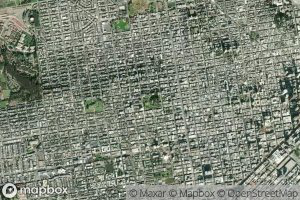
\includegraphics{images/san_francisco_scale_zoom_12.png}

}

}

\subcaption{\label{fig-sf}Downtown San Francisco}
\end{minipage}%
\newline
\begin{minipage}[t]{0.50\linewidth}

{\centering 

\raisebox{-\height}{

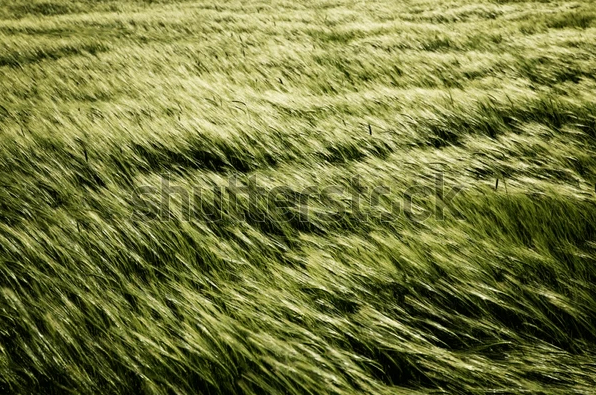
\includegraphics{images/grass_image2.jpg}

}

}

\subcaption{\label{fig-grass_internet}Internet Grass}
\end{minipage}%
%
\begin{minipage}[t]{0.50\linewidth}

{\centering 

\raisebox{-\height}{

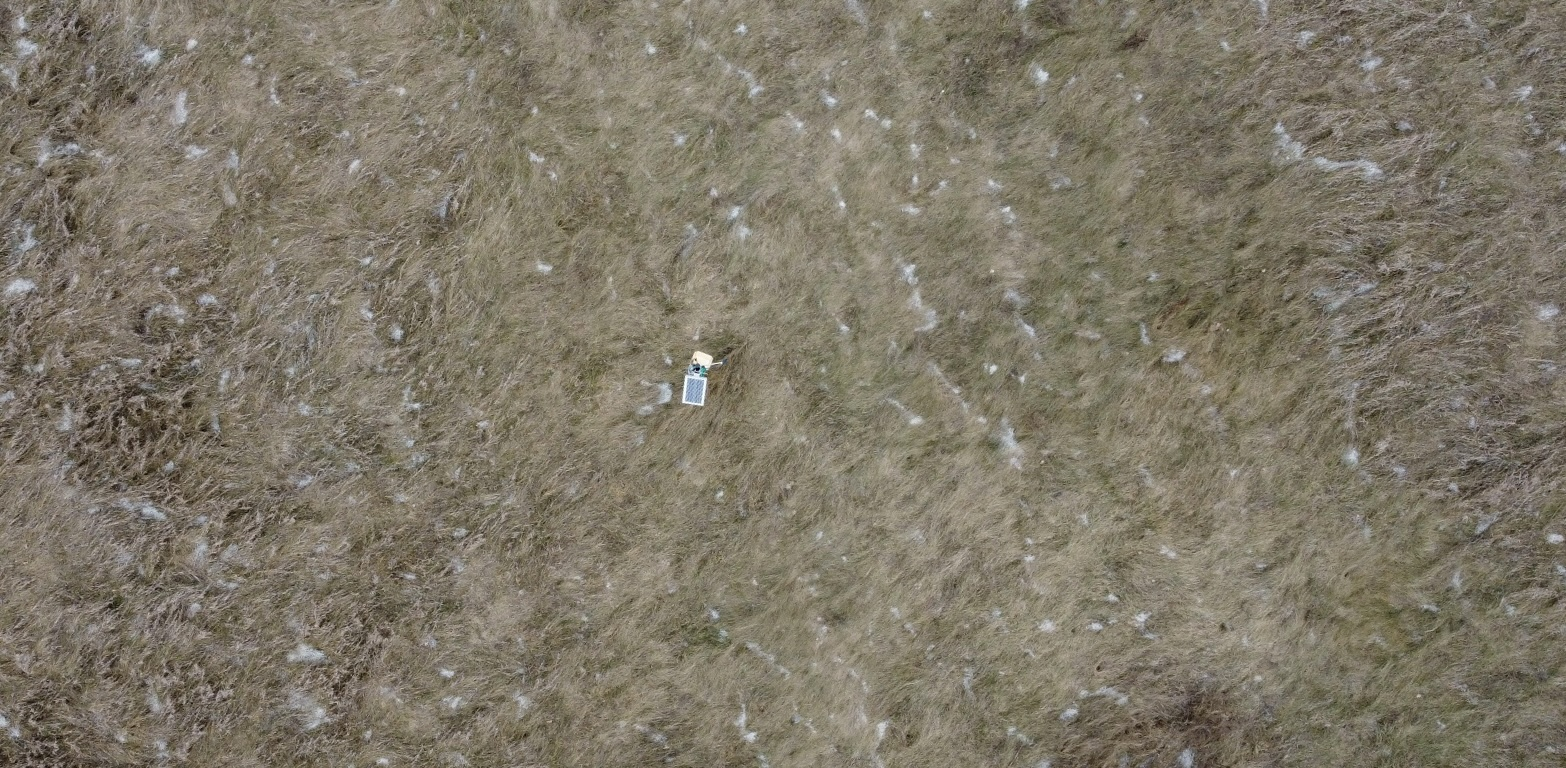
\includegraphics{images/living_lab_aerial/aerial_grass_living_lab_rotated.jpg}

}

}

\subcaption{\label{fig-living_labs}Aerial Living Labs}
\end{minipage}%

\caption{\label{fig-images}Featured Images for Evaluation}

\end{figure}

\bookmarksetup{startatroot}

\hypertarget{methods}{%
\chapter{Methods}\label{methods}}

~~~~~~The HOG algorithm, introduced by Navneet Dalal and Bill Triggs in
2005, is a popular technique for object detection in images. The
algorithm can identify gradient magnitudes and angles at each pixel in
an image. The preliminary steps involved using the `skimage' library
from Python to preprocess the images of interest. This included loading,
resizing, and converting the images to grayscale. Images were rescaled
to standardize their resolutions and preserve their aspect ratios to
prevent distortion that could affect the accuracy of angle
identification. Converting the images to grayscale was necessary because
it allowed for focusing on a single channel to represent pixel
intensity, rather than three channels (red, green, and blue).

\begin{figure}

\begin{minipage}[t]{\linewidth}

{\centering 

\raisebox{-\height}{

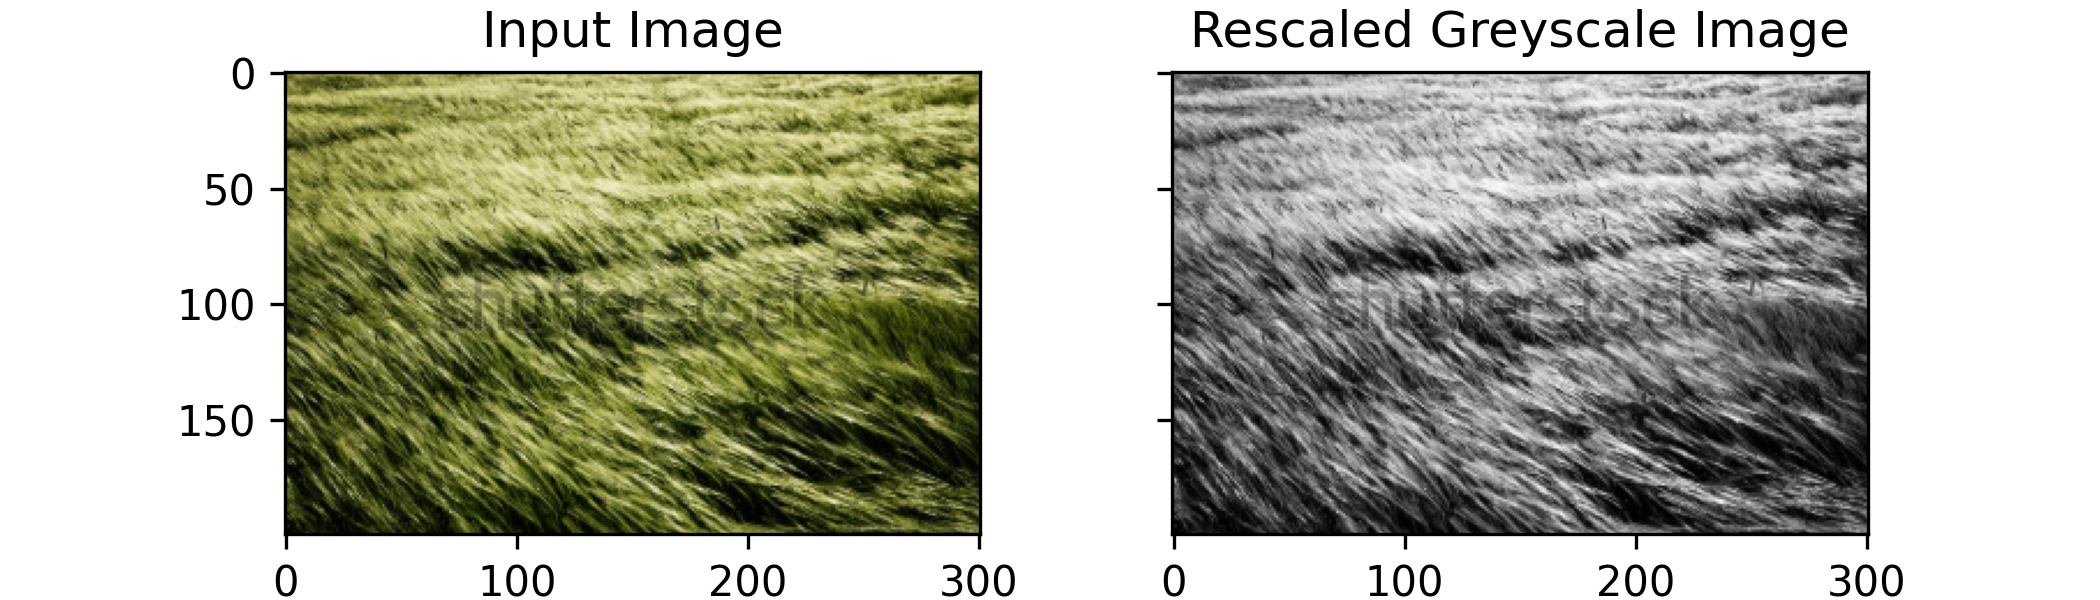
\includegraphics{images/plots/input_to_rescaled_plot.png}

}

}

\subcaption{\label{fig-input_image_to_new}Internet Grass Image}
\end{minipage}%

\caption{\label{fig-input_image}Rescaling and Converting Image to
Greyscale}

\end{figure}

~~~~~~The HOG features were then computed for the resized images, which
involved calculating the gradient magnitudes and angles at each pixel.
The gradient magnitude at each pixel is comprised of the gradients in
the `x' and `y' directions. The gradient in the x-direction is computed
by subtracting the pixel value to the left of pixel of interest is
subtracted from the pixel value to its right. Similarly, the gradient in
the y-direction is calculated by pixel value below the pixel of interest
is subtracted from the pixel value above the pixel of interest.

\(G_x=I(r,c+1)−I(r,c-1)\)

\(G_y=I(r+1,c)−I(r-1,c)\)

~~~~~~Now to calculate the gradient magnitude at the pixel of interest,
the Pythagorean Theorem can be utilized where the gradient magnitude is
equal to the square root of the x-gradient squared plus the y-gradient
squared. The angle at a given pixel can be calculated by taking the
inverse tangent of its y-gradient divided by its x-gradient. It is
important to note all angles produced by this algorithm are between zero
and one hundred eighty degrees. This occurs, because the inverse tangent
function used for calculating a given pixel's angle cannot distinguish
between all four quadrants.

\(Magnitude(\mu)=\sqrt{G_{x}^{2} + G_{y}^{2}}\)

\(Angle(\Theta)=tan^{−1} (\frac{G_y}{G_x})\)

\begin{figure}

\begin{minipage}[t]{\linewidth}

{\centering 

\raisebox{-\height}{

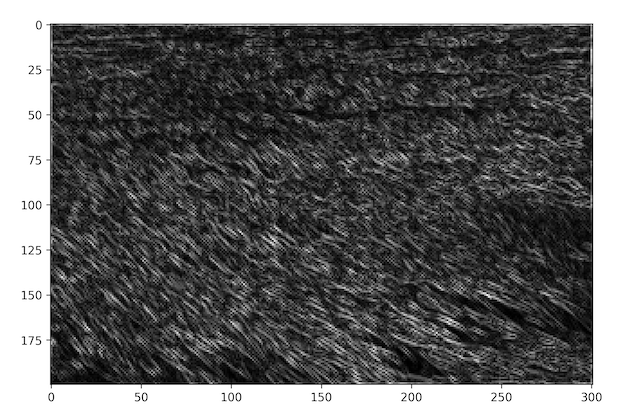
\includegraphics{images/plots/internet_grass_mag.png}

}

}

\subcaption{\label{fig-magnitude_grass}Internet Grass Image}
\end{minipage}%

\caption{\label{fig-mag_plot}Plotting Gradient Magnitudes}

\end{figure}

\hfill\break
~~~~~~Next, histograms are constructed to visualize the distribution of
gradient magnitudes and angles. Two different techniques for creating
gradient angle histograms were implemented. The first histogram was
created by counting the number of angles that fell into their respective
bins. The second scheme factors in a pixel's gradient magnitude and its
allocation to its bordering bins. Here, the weight assigned to each bin
is calculated by the angle's deviation from the center of its central
bin. This approach allows for a more representative histogram which
splits angles between bins and takes their magnitudes into account.
Lastly, these histograms are converted to polar histograms so the
primary angles can be visualized and compared to their original images.

\bookmarksetup{startatroot}

\hypertarget{results}{%
\chapter{Results}\label{results}}

\hypertarget{load-r-packages}{%
\section{Load R Packages}\label{load-r-packages}}

\begin{Shaded}
\begin{Highlighting}[]
\FunctionTok{library}\NormalTok{(reticulate)}
\FunctionTok{library}\NormalTok{(tidyverse)}
\end{Highlighting}
\end{Shaded}

\begin{verbatim}
-- Attaching core tidyverse packages ------------------------ tidyverse 2.0.0 --
v dplyr     1.1.2     v readr     2.1.4
v forcats   1.0.0     v stringr   1.5.0
v ggplot2   3.5.0     v tibble    3.2.1
v lubridate 1.9.2     v tidyr     1.3.0
v purrr     1.0.2     
-- Conflicts ------------------------------------------ tidyverse_conflicts() --
x dplyr::filter() masks stats::filter()
x dplyr::lag()    masks stats::lag()
i Use the conflicted package (<http://conflicted.r-lib.org/>) to force all conflicts to become errors
\end{verbatim}

\begin{Shaded}
\begin{Highlighting}[]
\FunctionTok{library}\NormalTok{(mapsapi)}
\FunctionTok{library}\NormalTok{(mapboxapi)}
\end{Highlighting}
\end{Shaded}

\begin{verbatim}
Usage of the Mapbox APIs is governed by the Mapbox Terms of Service.
Please visit https://www.mapbox.com/legal/tos/ for more information.
\end{verbatim}

\begin{Shaded}
\begin{Highlighting}[]
\FunctionTok{library}\NormalTok{(magick)}
\end{Highlighting}
\end{Shaded}

\begin{verbatim}
Linking to ImageMagick 6.9.12.93
Enabled features: cairo, fontconfig, freetype, heic, lcms, pango, raw, rsvg, webp
Disabled features: fftw, ghostscript, x11
\end{verbatim}

\begin{Shaded}
\begin{Highlighting}[]
\FunctionTok{Sys.which}\NormalTok{(}\StringTok{"python"}\NormalTok{)}
\end{Highlighting}
\end{Shaded}

\begin{verbatim}
                                                   python 
"/Users/bensunshine/.virtualenvs/r-reticulate/bin/python" 
\end{verbatim}

\hypertarget{download-aerial-city-images}{%
\section{Download Aerial City
Images}\label{download-aerial-city-images}}

\begin{Shaded}
\begin{Highlighting}[]
\NormalTok{key }\OtherTok{\textless{}{-}} \FunctionTok{Sys.getenv}\NormalTok{(}\StringTok{"mapbox\_key"}\NormalTok{)}
\end{Highlighting}
\end{Shaded}

\begin{Shaded}
\begin{Highlighting}[]
\NormalTok{map }\OtherTok{\textless{}{-}} \FunctionTok{static\_mapbox}\NormalTok{(}
  \AttributeTok{access\_token =}\NormalTok{ key,}
  \AttributeTok{style\_url =} \StringTok{"mapbox://styles/mapbox/satellite{-}v9"}\NormalTok{,}
  \AttributeTok{width =} \DecValTok{300}\NormalTok{,}
  \AttributeTok{height =} \DecValTok{200}\NormalTok{, }
  \AttributeTok{image =}\NormalTok{ T, }\AttributeTok{latitude =} \FloatTok{37.792004}\NormalTok{, }\AttributeTok{longitude =} \SpecialCharTok{{-}}\FloatTok{122.428079}\NormalTok{, }\AttributeTok{zoom =} \DecValTok{12}
\NormalTok{)}

\NormalTok{magick}\SpecialCharTok{::}\FunctionTok{image\_write}\NormalTok{(map, }\StringTok{"images/san\_francisco\_scale\_zoom\_12.png"}\NormalTok{)}
\end{Highlighting}
\end{Shaded}

\begin{Shaded}
\begin{Highlighting}[]
\NormalTok{points\_of\_interest }\OtherTok{\textless{}{-}}\NormalTok{ tibble}\SpecialCharTok{::}\FunctionTok{tibble}\NormalTok{(}
  \AttributeTok{longitude =} \FunctionTok{c}\NormalTok{(}\SpecialCharTok{{-}}\FloatTok{112.065945}\NormalTok{, }\SpecialCharTok{{-}}\FloatTok{111.853948}\NormalTok{, }
                \SpecialCharTok{{-}}\FloatTok{111.852956}\NormalTok{, }\SpecialCharTok{{-}}\FloatTok{112.023371}\NormalTok{),}
  
  \AttributeTok{latitude =} \FunctionTok{c}\NormalTok{(}\FloatTok{40.794275}\NormalTok{, }\FloatTok{40.791516}\NormalTok{, }
               \FloatTok{40.502308}\NormalTok{, }\FloatTok{40.502308}\NormalTok{)}
\NormalTok{  )}

\NormalTok{prepped\_pois }\OtherTok{\textless{}{-}} \FunctionTok{prep\_overlay\_markers}\NormalTok{(}
  \AttributeTok{data =}\NormalTok{ points\_of\_interest,}
  \AttributeTok{marker\_type =} \StringTok{"pin{-}l"}\NormalTok{,}
  \AttributeTok{label =} \DecValTok{1}\SpecialCharTok{:}\DecValTok{4}\NormalTok{,}
  \AttributeTok{color =} \StringTok{"\#fff"}\NormalTok{, }
\NormalTok{)}

\NormalTok{map }\OtherTok{\textless{}{-}} \FunctionTok{static\_mapbox}\NormalTok{(}
  \AttributeTok{access\_token =}\NormalTok{ key,}
  \AttributeTok{style\_url =} \StringTok{"mapbox://styles/mapbox/satellite{-}v9"}\NormalTok{,}
  \AttributeTok{width =} \DecValTok{800}\NormalTok{,}
  \AttributeTok{height =} \DecValTok{1200}\NormalTok{, }
  \AttributeTok{image =}\NormalTok{ T, }
  \AttributeTok{latitude =} \FloatTok{40.7}\NormalTok{,}
  \AttributeTok{longitude =} \SpecialCharTok{{-}}\FloatTok{111.876183}\NormalTok{, }\AttributeTok{zoom =} \DecValTok{12}
\NormalTok{)}

\NormalTok{magick}\SpecialCharTok{::}\FunctionTok{image\_write}\NormalTok{(map, }\StringTok{"images/salt\_lake\_city\_zoom\_12.png"}\NormalTok{)}
\end{Highlighting}
\end{Shaded}

\begin{Shaded}
\begin{Highlighting}[]
\NormalTok{map }\OtherTok{\textless{}{-}} \FunctionTok{static\_mapbox}\NormalTok{(}
  \AttributeTok{access\_token =}\NormalTok{ key,}
  \AttributeTok{style\_url =} \StringTok{"mapbox://styles/mapbox/satellite{-}v9"}\NormalTok{,}
  \AttributeTok{width =} \DecValTok{1200}\NormalTok{,}
  \AttributeTok{height =} \DecValTok{800}\NormalTok{, }
  \AttributeTok{image =}\NormalTok{ T, }
  \AttributeTok{latitude =} \FloatTok{42.336322}\NormalTok{,}
  \AttributeTok{longitude =} \SpecialCharTok{{-}}\FloatTok{83.048705}\NormalTok{, }\AttributeTok{zoom =} \DecValTok{12}
\NormalTok{)}

\NormalTok{magick}\SpecialCharTok{::}\FunctionTok{image\_write}\NormalTok{(map, }\StringTok{"images/detroit\_zoom\_12.png"}\NormalTok{)}
\end{Highlighting}
\end{Shaded}

\hypertarget{load-python-libraries}{%
\section{Load Python Libraries}\label{load-python-libraries}}

\begin{Shaded}
\begin{Highlighting}[]

\ImportTok{import}\NormalTok{ matplotlib.pyplot }\ImportTok{as}\NormalTok{ plt}
\ImportTok{import}\NormalTok{ pandas }\ImportTok{as}\NormalTok{ pd}

\CommentTok{\# jupyter only inline output command}
\CommentTok{\#\%matplotlib inline}

\ImportTok{from}\NormalTok{ skimage.io }\ImportTok{import}\NormalTok{ imread, imshow}
\ImportTok{from}\NormalTok{ skimage.transform }\ImportTok{import}\NormalTok{ resize}
\ImportTok{from}\NormalTok{ skimage.feature }\ImportTok{import}\NormalTok{ hog}
\ImportTok{from}\NormalTok{ skimage }\ImportTok{import}\NormalTok{ data, exposure}


\ImportTok{import}\NormalTok{ matplotlib.pyplot }\ImportTok{as}\NormalTok{ plt}
\ImportTok{from}\NormalTok{ skimage }\ImportTok{import}\NormalTok{ io}
\ImportTok{from}\NormalTok{ skimage }\ImportTok{import}\NormalTok{ color}
\ImportTok{from}\NormalTok{ skimage.transform }\ImportTok{import}\NormalTok{ resize}
\ImportTok{import}\NormalTok{ math}
\ImportTok{from}\NormalTok{ skimage.feature }\ImportTok{import}\NormalTok{ hog}
\ImportTok{import}\NormalTok{ numpy }\ImportTok{as}\NormalTok{ np}
\end{Highlighting}
\end{Shaded}

\hypertarget{collect-hog-features}{%
\section{Collect HOG Features}\label{collect-hog-features}}

\begin{Shaded}
\begin{Highlighting}[]
\NormalTok{img\_list }\OperatorTok{=}\NormalTok{ []}
\NormalTok{img\_list.append(color.rgb2gray(io.imread(}\StringTok{"images/diagnol\_lines.jpg"}\NormalTok{)))}
\NormalTok{img\_list.append(color.rgb2gray(io.imread(}\StringTok{"images/san\_francisco\_scale\_zoom\_12.png"}\NormalTok{)))}
\NormalTok{img\_list.append(color.rgb2gray(io.imread(}\StringTok{"images/grass\_image2.jpg"}\NormalTok{)))}
\NormalTok{img\_list.append(color.rgb2gray(io.imread(}\StringTok{"images/living\_lab\_aerial/aerial\_grass\_living\_lab\_rotated.jpg"}\NormalTok{)))}

\CommentTok{\#img = color.rgb2gray(io.imread("images/grass\_image2.jpg"))}

\CommentTok{\# img = color.rgb2gray(io.imread("images/b\_test\_image\_copy.jpg"))}
\CommentTok{\#img = color.rgb2gray(io.imread("images/long\_grass\_sample.jpeg"))}
\CommentTok{\#img = color.rgb2gray(io.imread("images/diagnol\_lines.jpg"))}

\CommentTok{\#img = color.rgb2gray(io.imread("images/san\_francisco\_scale\_zoom\_12.png"))}

\CommentTok{\#img = color.rgb2gray(io.imread("images/diagnol\_lines\_flipped.jpg"))}
\CommentTok{\#img = color.rgb2gray(io.imread("images/long\_grass\_sample\_cropped.jpg"))}

\CommentTok{\# aerial rotated image}
\CommentTok{\#img = color.rgb2gray(io.imread("images/living\_lab\_aerial/aerial\_grass\_living\_lab\_rotated.jpg"))}

\CommentTok{\# zoomed internet photo}
\CommentTok{\#img = color.rgb2gray(io.imread("images/dead\_grass\_zoom.jpeg"))}


\CommentTok{\# zoomed in 11}
\CommentTok{\#img = color.rgb2gray(io.imread("images/living\_lab\_aerial/LL\_zoomed\_in\_11.jpg"))}

\CommentTok{\# zoomed in 12}
\CommentTok{\#img = color.rgb2gray(io.imread("images/living\_lab\_aerial/LL\_zoomed\_in\_12.jpg"))}

\CommentTok{\# zoomed in 16}
\CommentTok{\#img = color.rgb2gray(io.imread("images/living\_lab\_aerial/LL\_zoomed\_in\_16\_side.jpg"))}



\CommentTok{\# real one}
\CommentTok{\#img = color.rgb2gray(io.imread("images/living\_labs\_real\_grass\_image.jpg"))}

\NormalTok{mag\_list }\OperatorTok{=}\NormalTok{ []}
\NormalTok{theta\_list }\OperatorTok{=}\NormalTok{ []}


\ControlFlowTok{for}\NormalTok{ x }\KeywordTok{in} \BuiltInTok{range}\NormalTok{(}\BuiltInTok{len}\NormalTok{(img\_list)):}
\NormalTok{    img }\OperatorTok{=}\NormalTok{ img\_list[x]}
    
\NormalTok{    aspect\_ratio }\OperatorTok{=}\NormalTok{ img.shape[}\DecValTok{0}\NormalTok{] }\OperatorTok{/}\NormalTok{ img.shape[}\DecValTok{1}\NormalTok{]}
    \BuiltInTok{print}\NormalTok{(}\StringTok{"Aspect Ratio:"}\NormalTok{, aspect\_ratio)}
    
\NormalTok{    height }\OperatorTok{=} \DecValTok{200}
\NormalTok{    width }\OperatorTok{=} \BuiltInTok{int}\NormalTok{(height }\OperatorTok{/}\NormalTok{ aspect\_ratio)}
    \BuiltInTok{print}\NormalTok{(}\StringTok{"Resized Width:"}\NormalTok{, width)}
    
\NormalTok{    resized\_img }\OperatorTok{=}\NormalTok{ resize(img, (height, width))}
\NormalTok{    img\_list[x] }\OperatorTok{=}\NormalTok{ resized\_img}
    
\NormalTok{    plt.figure(figsize}\OperatorTok{=}\NormalTok{(}\DecValTok{15}\NormalTok{, }\DecValTok{8}\NormalTok{))}
\NormalTok{    plt.imshow(resized\_img, cmap}\OperatorTok{=}\StringTok{"gray"}\NormalTok{)}
\NormalTok{    plt.axis(}\StringTok{"off"}\NormalTok{)}
\NormalTok{    plt.show()}
    
\NormalTok{    mag }\OperatorTok{=}\NormalTok{ []}
\NormalTok{    theta }\OperatorTok{=}\NormalTok{ []}
    
    \ControlFlowTok{for}\NormalTok{ i }\KeywordTok{in} \BuiltInTok{range}\NormalTok{(height):}
\NormalTok{        magnitudeArray }\OperatorTok{=}\NormalTok{ []}
\NormalTok{        angleArray }\OperatorTok{=}\NormalTok{ []}
        
        \ControlFlowTok{for}\NormalTok{ j }\KeywordTok{in} \BuiltInTok{range}\NormalTok{(width):}
            \ControlFlowTok{if}\NormalTok{ j }\OperatorTok{{-}} \DecValTok{1} \OperatorTok{\textless{}} \DecValTok{0} \KeywordTok{or}\NormalTok{ j }\OperatorTok{+} \DecValTok{1} \OperatorTok{\textgreater{}=}\NormalTok{ width:}
                \ControlFlowTok{if}\NormalTok{ j }\OperatorTok{{-}} \DecValTok{1} \OperatorTok{\textless{}} \DecValTok{0}\NormalTok{:}
\NormalTok{                    Gx }\OperatorTok{=}\NormalTok{ img[i][j }\OperatorTok{+} \DecValTok{1}\NormalTok{] }\OperatorTok{{-}} \DecValTok{0}
                \ControlFlowTok{elif}\NormalTok{ j }\OperatorTok{+} \DecValTok{1} \OperatorTok{\textgreater{}=}\NormalTok{ width:}
\NormalTok{                    Gx }\OperatorTok{=} \DecValTok{0} \OperatorTok{{-}}\NormalTok{ img[i][j }\OperatorTok{{-}} \DecValTok{1}\NormalTok{]}
            \ControlFlowTok{else}\NormalTok{:}
\NormalTok{                Gx }\OperatorTok{=}\NormalTok{ img[i][j }\OperatorTok{+} \DecValTok{1}\NormalTok{] }\OperatorTok{{-}}\NormalTok{ img[i][j }\OperatorTok{{-}} \DecValTok{1}\NormalTok{]}
                
            \ControlFlowTok{if}\NormalTok{ i }\OperatorTok{{-}} \DecValTok{1} \OperatorTok{\textless{}} \DecValTok{0} \KeywordTok{or}\NormalTok{ i }\OperatorTok{+} \DecValTok{1} \OperatorTok{\textgreater{}=}\NormalTok{ height:}
                \ControlFlowTok{if}\NormalTok{ i }\OperatorTok{{-}} \DecValTok{1} \OperatorTok{\textless{}} \DecValTok{0}\NormalTok{:}
\NormalTok{                    Gy }\OperatorTok{=} \DecValTok{0} \OperatorTok{{-}}\NormalTok{ img[i }\OperatorTok{+} \DecValTok{1}\NormalTok{][j]}
                \ControlFlowTok{elif}\NormalTok{ i }\OperatorTok{+} \DecValTok{1} \OperatorTok{\textgreater{}=}\NormalTok{ height:}
\NormalTok{                    Gy }\OperatorTok{=}\NormalTok{ img[i }\OperatorTok{{-}} \DecValTok{1}\NormalTok{][j] }\OperatorTok{{-}} \DecValTok{0}
            \ControlFlowTok{else}\NormalTok{:}
\NormalTok{                Gy }\OperatorTok{=}\NormalTok{ img[i }\OperatorTok{+} \DecValTok{1}\NormalTok{][j] }\OperatorTok{{-}}\NormalTok{ img[i }\OperatorTok{{-}} \DecValTok{1}\NormalTok{][j]}
                
\NormalTok{            magnitude }\OperatorTok{=}\NormalTok{ math.sqrt(}\BuiltInTok{pow}\NormalTok{(Gx, }\DecValTok{2}\NormalTok{) }\OperatorTok{+} \BuiltInTok{pow}\NormalTok{(Gy, }\DecValTok{2}\NormalTok{))}
\NormalTok{            magnitudeArray.append(}\BuiltInTok{round}\NormalTok{(magnitude, }\DecValTok{9}\NormalTok{))}
            
            \ControlFlowTok{if}\NormalTok{ Gx }\OperatorTok{==} \DecValTok{0}\NormalTok{:}
\NormalTok{                angle }\OperatorTok{=}\NormalTok{ math.degrees(}\FloatTok{0.0}\NormalTok{)}
            \ControlFlowTok{else}\NormalTok{:}
\NormalTok{                angle }\OperatorTok{=}\NormalTok{ math.degrees(math.atan(Gy }\OperatorTok{/}\NormalTok{ Gx))}
                \ControlFlowTok{if}\NormalTok{ angle }\OperatorTok{\textless{}} \DecValTok{0}\NormalTok{:}
\NormalTok{                    angle }\OperatorTok{+=} \DecValTok{180}
                    
\NormalTok{            angleArray.append(}\BuiltInTok{round}\NormalTok{(angle, }\DecValTok{9}\NormalTok{))}
            
\NormalTok{        mag.append(magnitudeArray)}
\NormalTok{        theta.append(angleArray)}
        
\NormalTok{    mag\_list.append(mag)}
\NormalTok{    theta\_list.append(theta)}
\end{Highlighting}
\end{Shaded}

\begin{verbatim}
Aspect Ratio: 1.0
Resized Width: 200
<Figure size 3000x1600 with 0 Axes>
<matplotlib.image.AxesImage object at 0x292a43250>
(-0.5, 199.5, 199.5, -0.5)
Aspect Ratio: 0.6666666666666666
Resized Width: 300
<Figure size 3000x1600 with 0 Axes>
<matplotlib.image.AxesImage object at 0x2c418b850>
(-0.5, 299.5, 199.5, -0.5)
Aspect Ratio: 0.662751677852349
Resized Width: 301
<Figure size 3000x1600 with 0 Axes>
<matplotlib.image.AxesImage object at 0x2c874af90>
(-0.5, 300.5, 199.5, -0.5)
Aspect Ratio: 0.4904214559386973
Resized Width: 407
<Figure size 3000x1600 with 0 Axes>
<matplotlib.image.AxesImage object at 0x2dcc55690>
(-0.5, 406.5, 199.5, -0.5)
\end{verbatim}

\begin{figure}[H]

{\centering 
\includegraphics{results_files/figure-pdf/unnamed-chunk-5-1.pdf}

}

\end{figure}

\begin{figure}[H]

{\centering 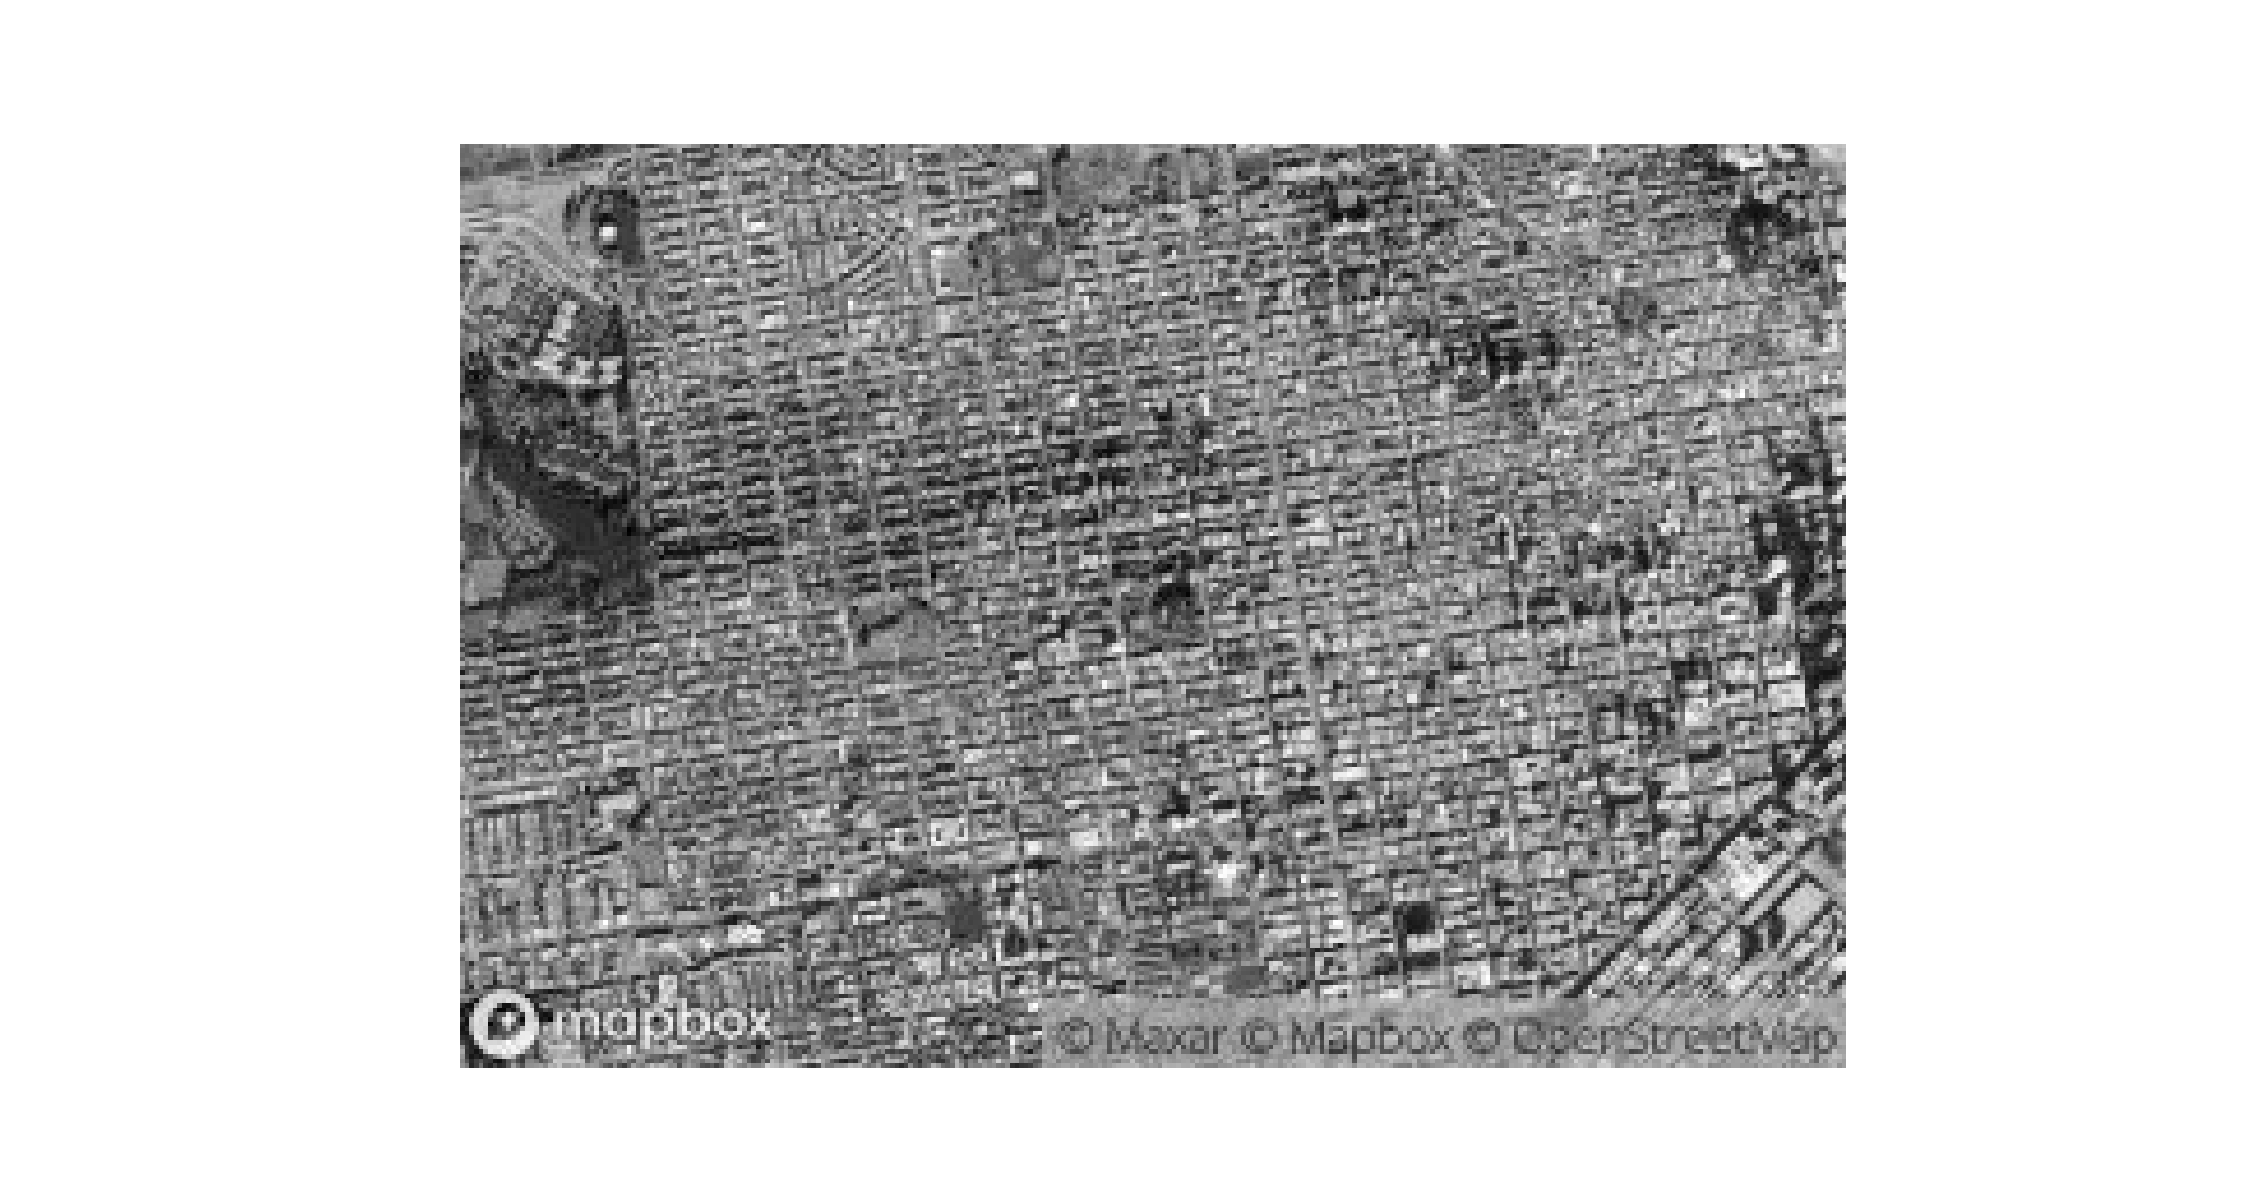
\includegraphics{results_files/figure-pdf/unnamed-chunk-5-2.pdf}

}

\end{figure}

\begin{figure}[H]

{\centering 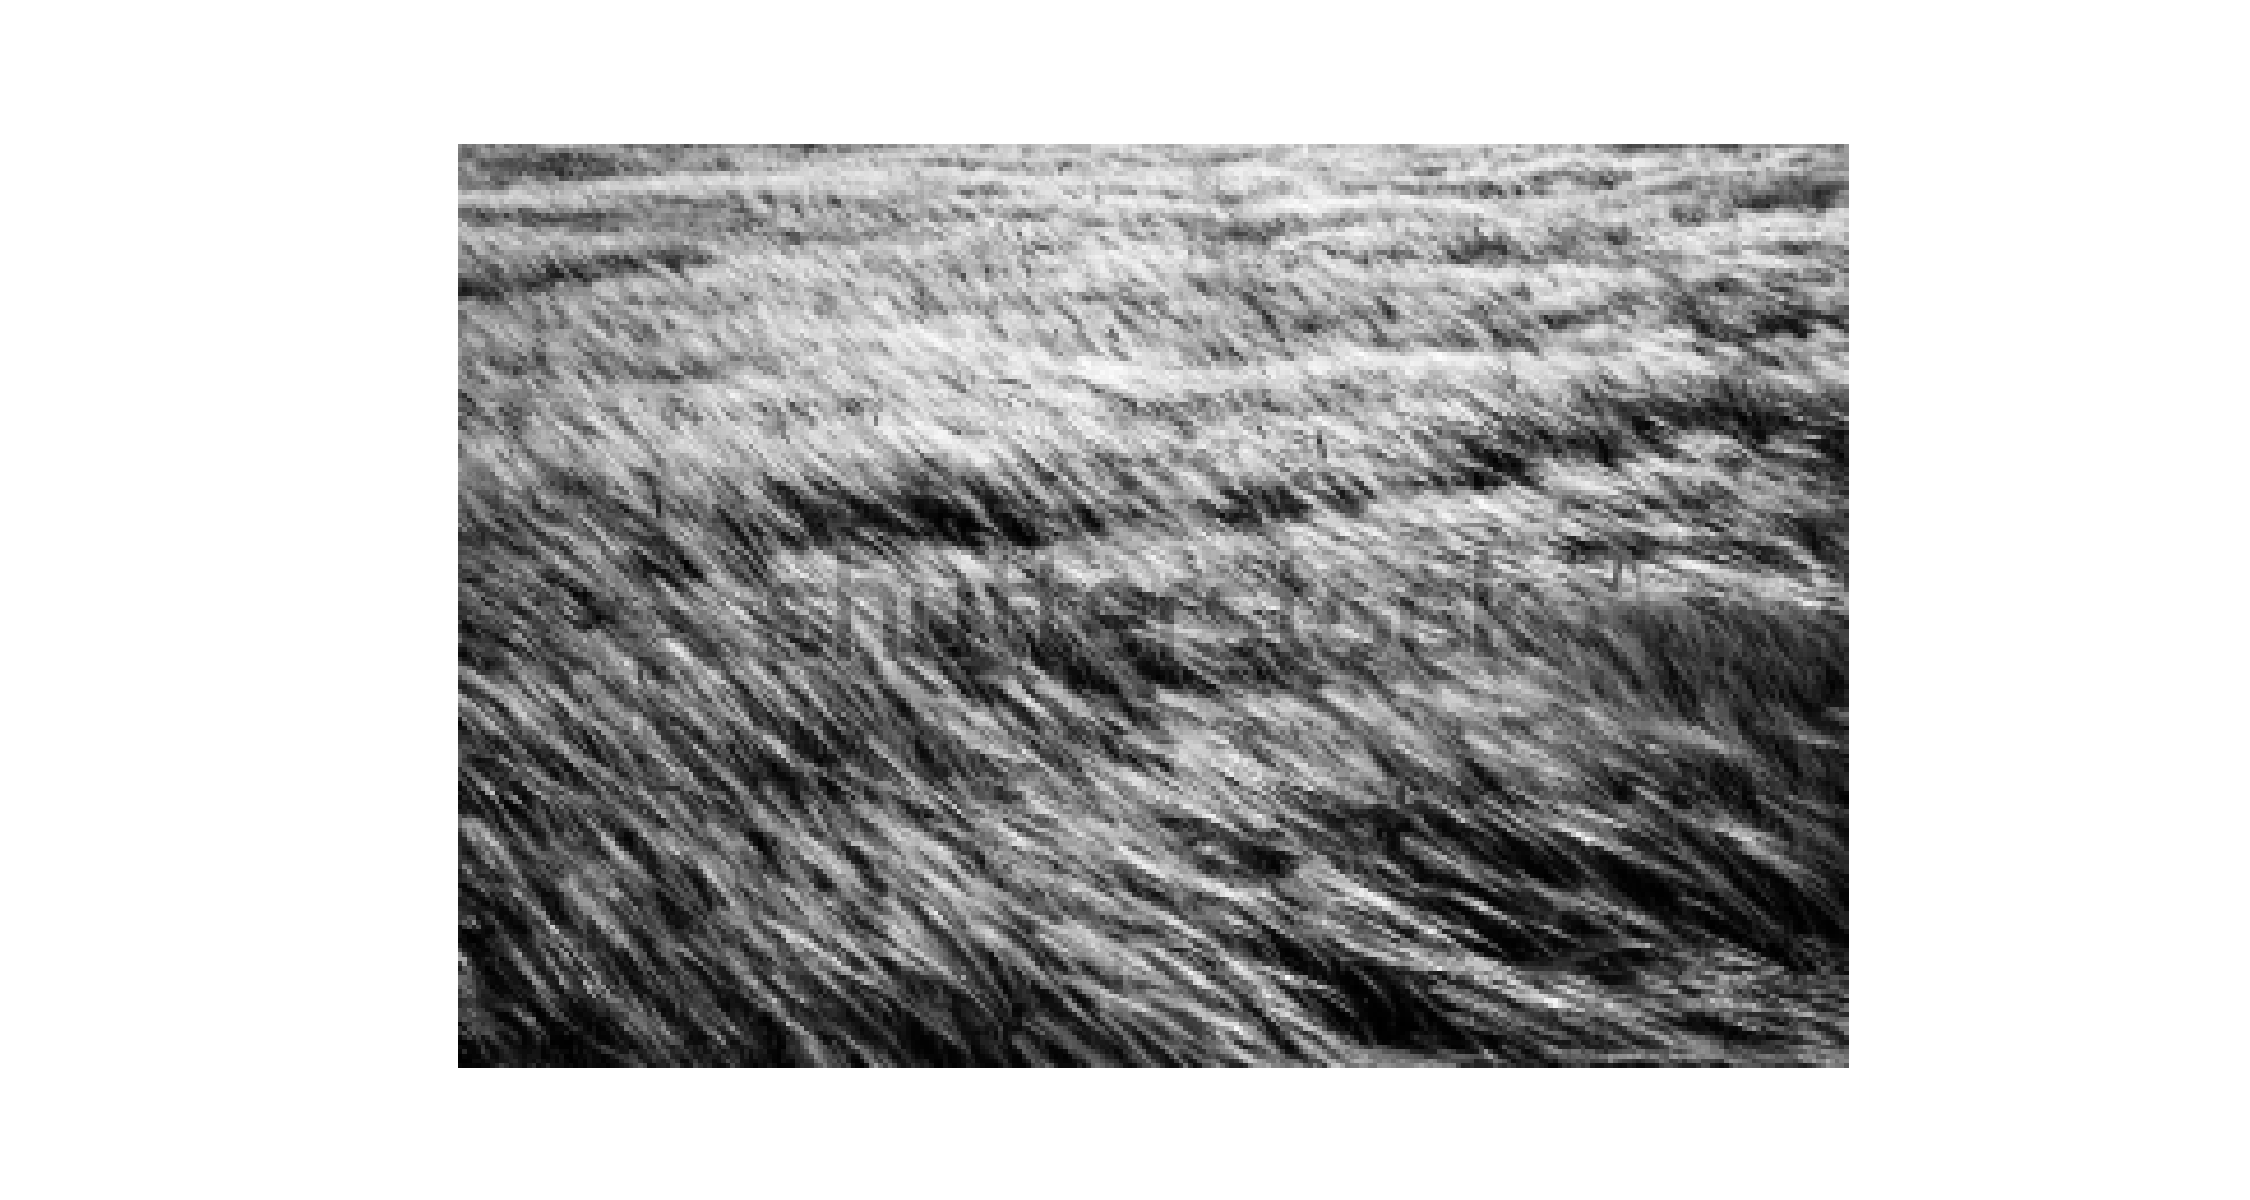
\includegraphics{results_files/figure-pdf/unnamed-chunk-5-3.pdf}

}

\end{figure}

\begin{figure}[H]

{\centering 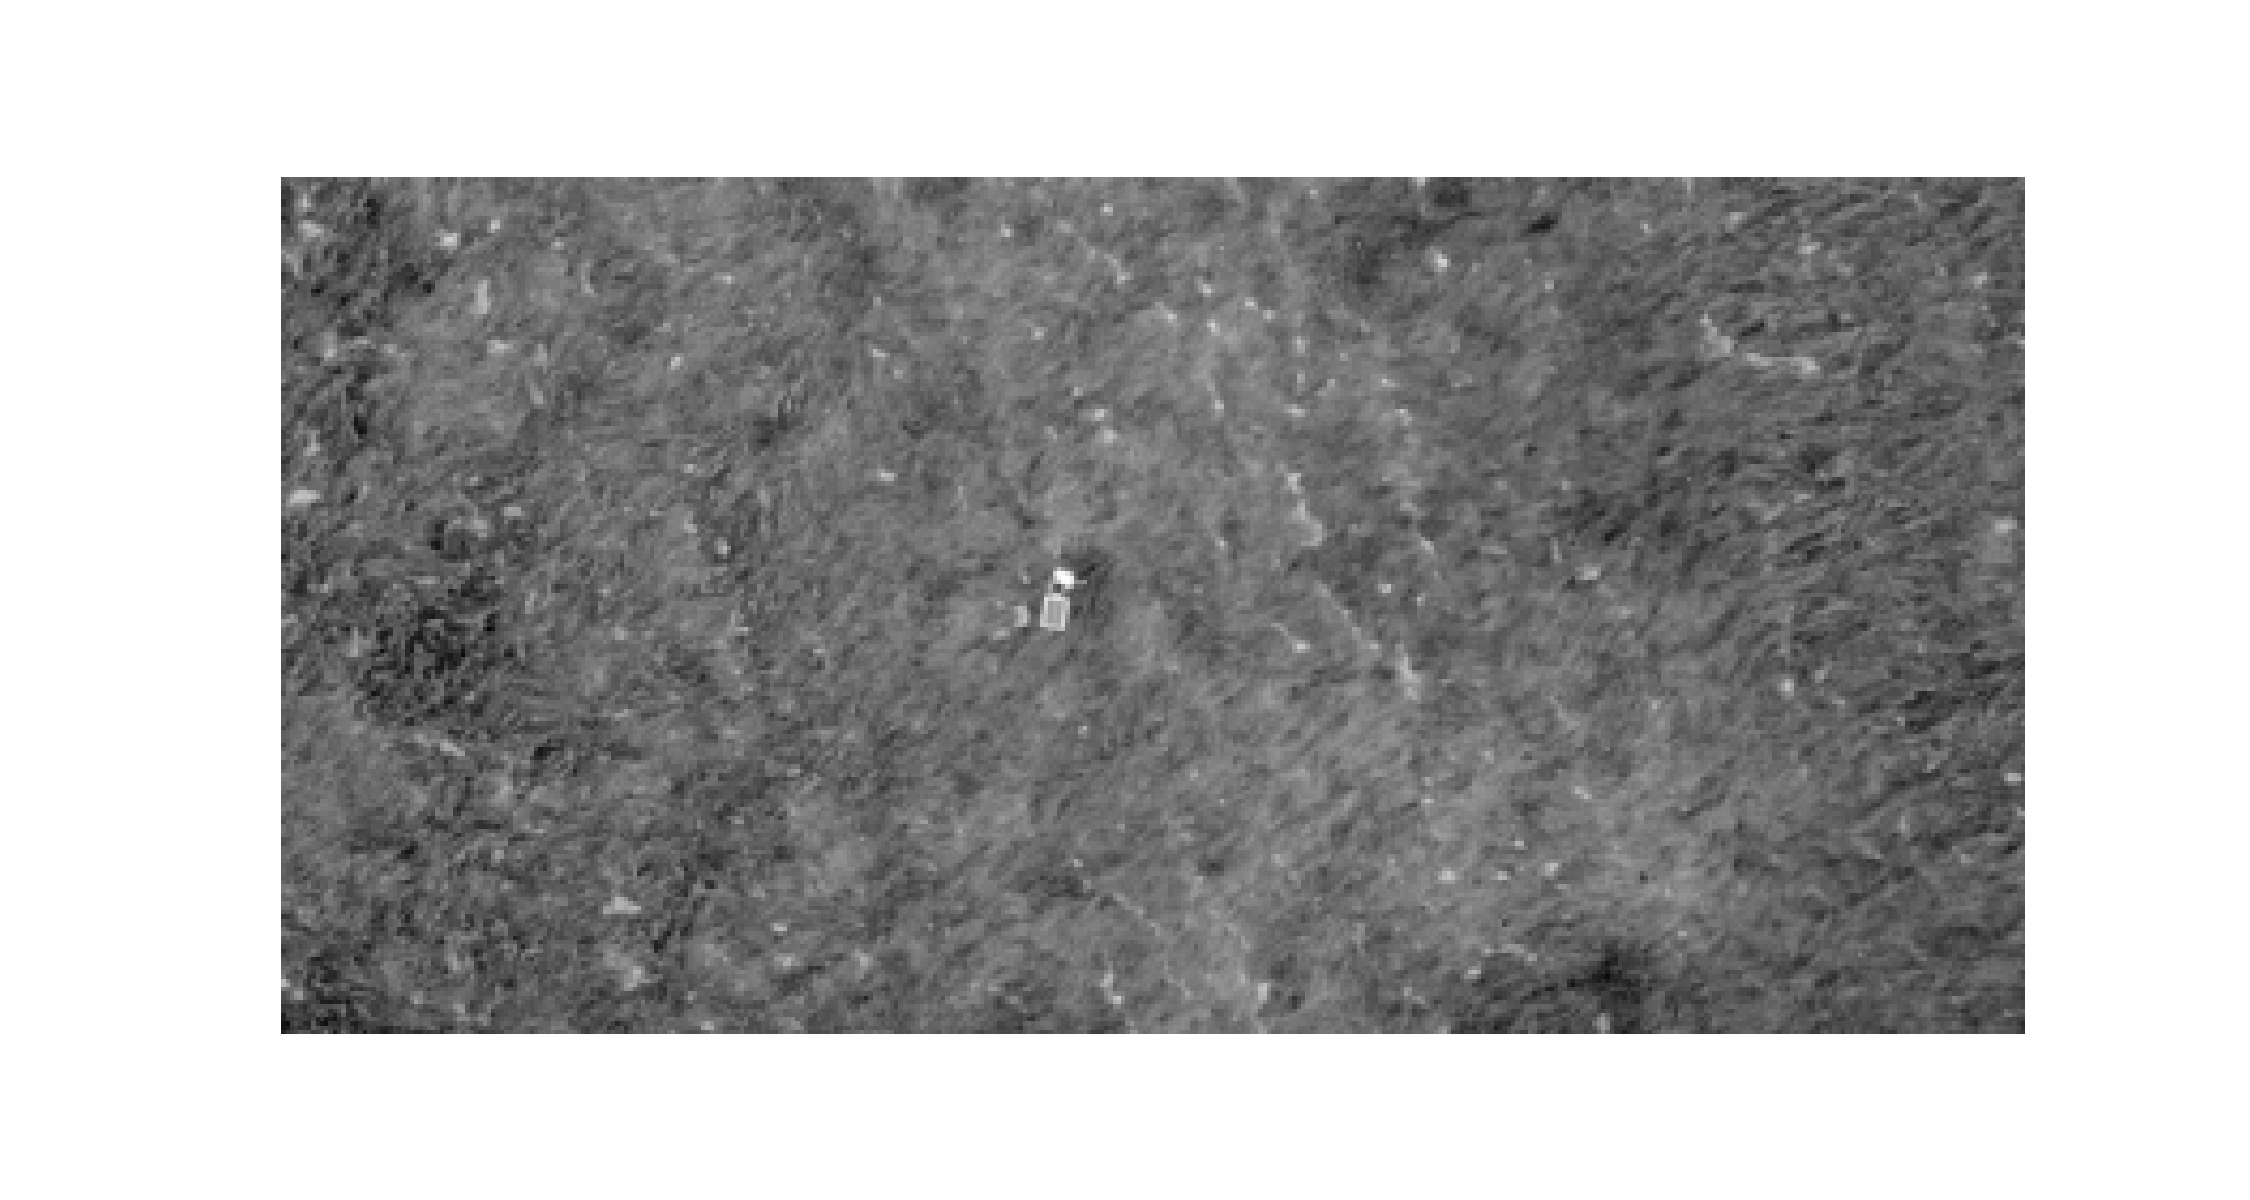
\includegraphics{results_files/figure-pdf/unnamed-chunk-5-4.pdf}

}

\end{figure}

\hypertarget{build-data-frames-for-each-image}{%
\section{Build Data Frames for Each
Image}\label{build-data-frames-for-each-image}}

\begin{Shaded}
\begin{Highlighting}[]
\NormalTok{mag\_diagonal }\OperatorTok{=}\NormalTok{ np.array(mag\_list[}\DecValTok{0}\NormalTok{])}
\NormalTok{theta\_diagonal }\OperatorTok{=}\NormalTok{ np.array(theta\_list[}\DecValTok{0}\NormalTok{])}


\NormalTok{mag\_sf }\OperatorTok{=}\NormalTok{ np.array(mag\_list[}\DecValTok{1}\NormalTok{])}
\NormalTok{theta\_sf }\OperatorTok{=}\NormalTok{ np.array(theta\_list[}\DecValTok{1}\NormalTok{])}


\NormalTok{mag\_internet\_grass }\OperatorTok{=}\NormalTok{ np.array(mag\_list[}\DecValTok{2}\NormalTok{])}
\NormalTok{theta\_internet\_grass }\OperatorTok{=}\NormalTok{ np.array(theta\_list[}\DecValTok{2}\NormalTok{])}


\NormalTok{mag\_living\_labs }\OperatorTok{=}\NormalTok{ np.array(mag\_list[}\DecValTok{3}\NormalTok{])}
\NormalTok{theta\_living\_labs }\OperatorTok{=}\NormalTok{ np.array(theta\_list[}\DecValTok{3}\NormalTok{])}
\end{Highlighting}
\end{Shaded}

\begin{Shaded}
\begin{Highlighting}[]
\CommentTok{\# Diagonal DF}
\NormalTok{diagonal\_hog\_df }\OtherTok{\textless{}{-}} \FunctionTok{data.frame}\NormalTok{(}\AttributeTok{mag =} \FunctionTok{as.vector}\NormalTok{(py}\SpecialCharTok{$}\NormalTok{mag\_diagonal),}
                              \AttributeTok{theta =} \FunctionTok{as.vector}\NormalTok{((py}\SpecialCharTok{$}\NormalTok{theta\_diagonal))) }\SpecialCharTok{\%\textgreater{}\%}
  \FunctionTok{mutate}\NormalTok{(}\AttributeTok{radian =}\NormalTok{ theta}\SpecialCharTok{*}\NormalTok{(pi}\SpecialCharTok{/}\DecValTok{180}\NormalTok{))}

\CommentTok{\# San Francisco DF}
\NormalTok{sf\_hog\_df }\OtherTok{\textless{}{-}} \FunctionTok{data.frame}\NormalTok{(}\AttributeTok{mag =} \FunctionTok{as.vector}\NormalTok{(py}\SpecialCharTok{$}\NormalTok{mag\_sf),}
                              \AttributeTok{theta =} \FunctionTok{as.vector}\NormalTok{((py}\SpecialCharTok{$}\NormalTok{theta\_sf))) }\SpecialCharTok{\%\textgreater{}\%}
  \FunctionTok{mutate}\NormalTok{(}\AttributeTok{radian =}\NormalTok{ theta}\SpecialCharTok{*}\NormalTok{(pi}\SpecialCharTok{/}\DecValTok{180}\NormalTok{))}

\CommentTok{\# Internet Grass DF}
\NormalTok{internet\_grass\_hog\_df }\OtherTok{\textless{}{-}} \FunctionTok{data.frame}\NormalTok{(}\AttributeTok{mag =} \FunctionTok{as.vector}\NormalTok{(py}\SpecialCharTok{$}\NormalTok{mag\_internet\_grass),}
                              \AttributeTok{theta =} \FunctionTok{as.vector}\NormalTok{((py}\SpecialCharTok{$}\NormalTok{theta\_internet\_grass))) }\SpecialCharTok{\%\textgreater{}\%}
  \FunctionTok{mutate}\NormalTok{(}\AttributeTok{radian =}\NormalTok{ theta}\SpecialCharTok{*}\NormalTok{(pi}\SpecialCharTok{/}\DecValTok{180}\NormalTok{))}

\CommentTok{\# Living Labs DF}
\NormalTok{living\_labs\_hog\_df }\OtherTok{\textless{}{-}} \FunctionTok{data.frame}\NormalTok{(}\AttributeTok{mag =} \FunctionTok{as.vector}\NormalTok{(py}\SpecialCharTok{$}\NormalTok{mag\_living\_labs),}
                              \AttributeTok{theta =} \FunctionTok{as.vector}\NormalTok{((py}\SpecialCharTok{$}\NormalTok{theta\_living\_labs))) }\SpecialCharTok{\%\textgreater{}\%}
  \FunctionTok{mutate}\NormalTok{(}\AttributeTok{radian =}\NormalTok{ theta}\SpecialCharTok{*}\NormalTok{(pi}\SpecialCharTok{/}\DecValTok{180}\NormalTok{))}

\CommentTok{\# List of all Data frames}
\NormalTok{standard\_df\_list }\OtherTok{=} \FunctionTok{list}\NormalTok{(diagonal\_hog\_df,}
\NormalTok{                        sf\_hog\_df, }
\NormalTok{                        internet\_grass\_hog\_df, }
\NormalTok{                        living\_labs\_hog\_df)}
\end{Highlighting}
\end{Shaded}

\hypertarget{plot-magnitudes-as-image}{%
\section{Plot Magnitudes as Image}\label{plot-magnitudes-as-image}}

\begin{Shaded}
\begin{Highlighting}[]
\NormalTok{plt.figure(figsize}\OperatorTok{=}\NormalTok{(}\DecValTok{15}\NormalTok{, }\DecValTok{8}\NormalTok{))}
\NormalTok{plt.title(}\StringTok{\textquotesingle{}Gradient Magnitudes\textquotesingle{}}\NormalTok{)}
\NormalTok{plt.imshow(mag\_list[}\DecValTok{0}\NormalTok{], cmap}\OperatorTok{=}\StringTok{"gray"}\NormalTok{)}
\NormalTok{plt.axis(}\StringTok{"off"}\NormalTok{)}
\end{Highlighting}
\end{Shaded}

\begin{verbatim}
(-0.5, 199.5, 199.5, -0.5)
\end{verbatim}

\begin{Shaded}
\begin{Highlighting}[]
\NormalTok{plt.show()}
\end{Highlighting}
\end{Shaded}

\begin{figure}[H]

{\centering 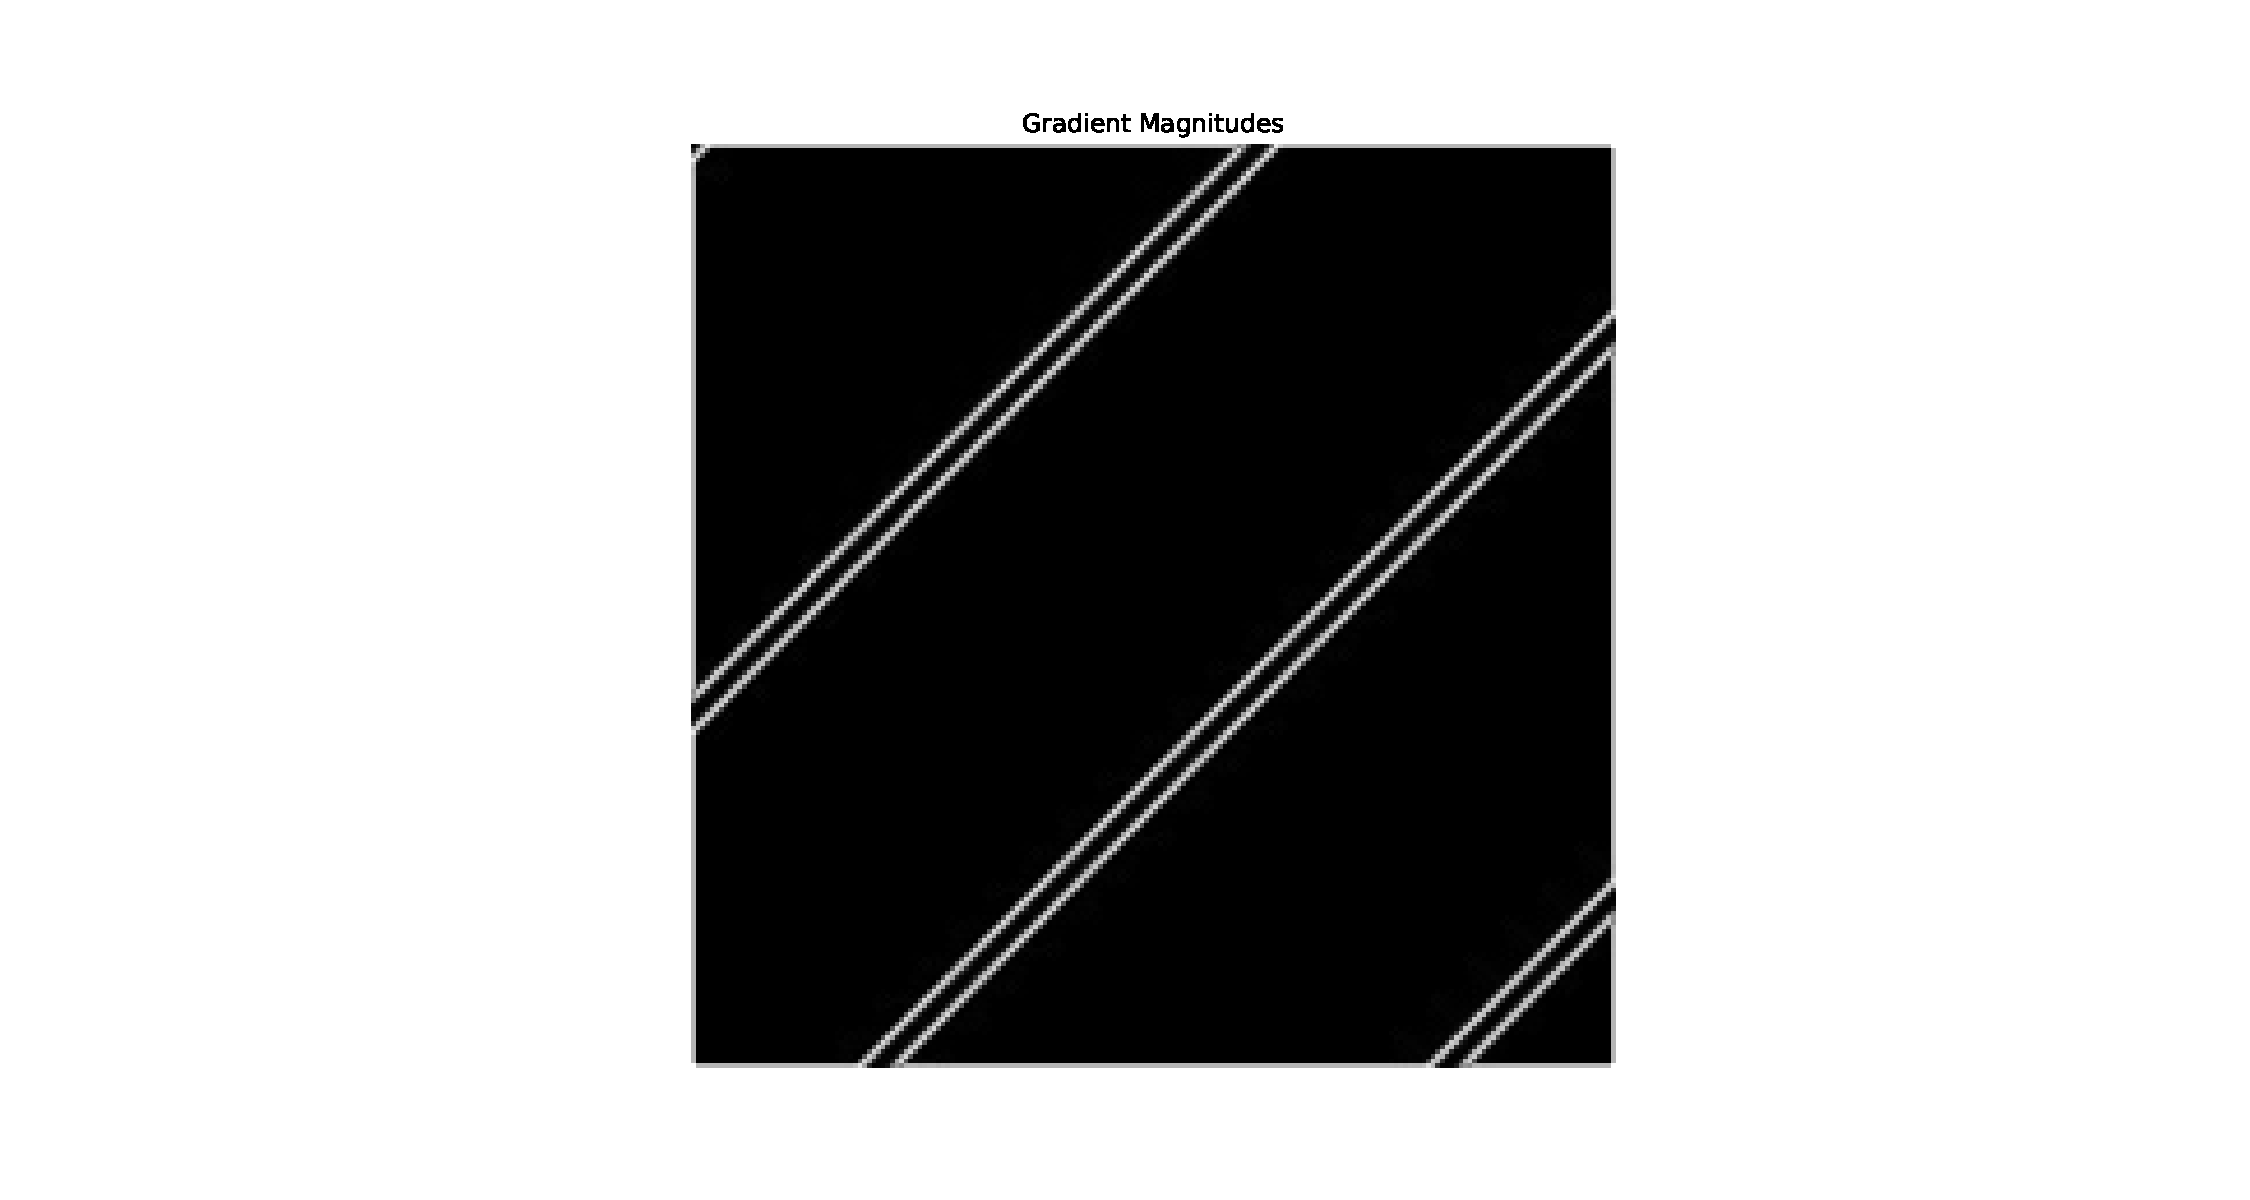
\includegraphics{results_files/figure-pdf/unnamed-chunk-8-1.pdf}

}

\end{figure}

\begin{Shaded}
\begin{Highlighting}[]

\NormalTok{plt.savefig(}\StringTok{"mag.png"}\NormalTok{, dpi}\OperatorTok{=}\DecValTok{300}\NormalTok{)}
\end{Highlighting}
\end{Shaded}

\begin{figure}[H]

{\centering 
\includegraphics{results_files/figure-pdf/unnamed-chunk-8-2.pdf}

}

\end{figure}

\hypertarget{create-histogram-plots-of-gradient-magnitudes-and-angles}{%
\section{Create Histogram Plots of Gradient Magnitudes and
Angles}\label{create-histogram-plots-of-gradient-magnitudes-and-angles}}

\begin{Shaded}
\begin{Highlighting}[]
\NormalTok{diagonal\_histogram\_mag\_plot }\OtherTok{\textless{}{-}}
  \FunctionTok{ggplot}\NormalTok{(standard\_df\_list[[}\DecValTok{1}\NormalTok{]], }
         \FunctionTok{aes}\NormalTok{(}\AttributeTok{x =}\NormalTok{ mag)) }\SpecialCharTok{+}
  \FunctionTok{geom\_histogram}\NormalTok{(}\AttributeTok{colour =} \StringTok{"black"}\NormalTok{, }\AttributeTok{fill =} \StringTok{"lightblue"}\NormalTok{) }\SpecialCharTok{+}
  \FunctionTok{scale\_x\_continuous}\NormalTok{() }\SpecialCharTok{+} 
  \FunctionTok{labs}\NormalTok{(}\AttributeTok{x =} \StringTok{"Gradient Magnitude"}\NormalTok{, }
       \AttributeTok{y =} \StringTok{"Count"}\NormalTok{, }
       \AttributeTok{title =} \StringTok{"Diagonal Line Image Histogram of Gradient Magnitudes"}
\NormalTok{       ) }\SpecialCharTok{+}
  \FunctionTok{theme\_minimal}\NormalTok{() }\SpecialCharTok{+}
  \FunctionTok{theme}\NormalTok{(}\AttributeTok{plot.title =} \FunctionTok{element\_text}\NormalTok{(}\AttributeTok{hjust =} \FloatTok{0.5}\NormalTok{))}

\NormalTok{diagonal\_histogram\_mag\_plot}
\end{Highlighting}
\end{Shaded}

\begin{verbatim}
`stat_bin()` using `bins = 30`. Pick better value with `binwidth`.
\end{verbatim}

\begin{figure}[H]

{\centering 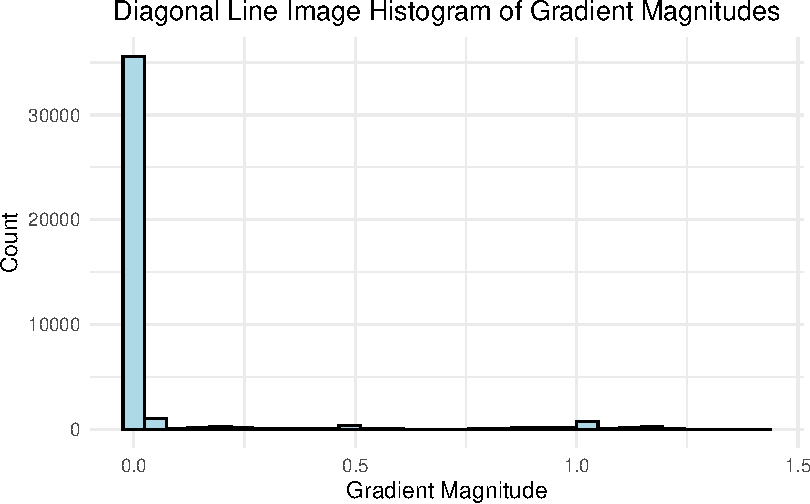
\includegraphics{results_files/figure-pdf/unnamed-chunk-9-5.pdf}

}

\end{figure}

\begin{Shaded}
\begin{Highlighting}[]
\NormalTok{diagonal\_mag\_filter }\OtherTok{\textless{}{-}} \FloatTok{0.1}

\FunctionTok{ggsave}\NormalTok{(}\StringTok{"images/plots/diagonal\_histogram\_mag\_plot.jpg"}\NormalTok{, diagonal\_histogram\_mag\_plot, }\AttributeTok{width =} \DecValTok{6}\NormalTok{, }\AttributeTok{height =} \DecValTok{4}\NormalTok{, }\AttributeTok{dpi =} \DecValTok{300}\NormalTok{)}
\end{Highlighting}
\end{Shaded}

\begin{verbatim}
`stat_bin()` using `bins = 30`. Pick better value with `binwidth`.
\end{verbatim}

\begin{Shaded}
\begin{Highlighting}[]
\NormalTok{diagonal\_histogram\_theta\_plot }\OtherTok{\textless{}{-}}
  \FunctionTok{ggplot}\NormalTok{(standard\_df\_list[[}\DecValTok{1}\NormalTok{]], }
         \FunctionTok{aes}\NormalTok{(}\AttributeTok{x =}\NormalTok{ theta)) }\SpecialCharTok{+}
  \FunctionTok{geom\_histogram}\NormalTok{(}\AttributeTok{colour =} \StringTok{"black"}\NormalTok{, }\AttributeTok{fill =} \StringTok{"lightblue"}\NormalTok{) }\SpecialCharTok{+}
  \FunctionTok{scale\_x\_continuous}\NormalTok{() }\SpecialCharTok{+} 
  \FunctionTok{labs}\NormalTok{(}\AttributeTok{x =} \StringTok{"Gradient Angle"}\NormalTok{, }
       \AttributeTok{y =} \StringTok{"Count"}\NormalTok{, }
       \AttributeTok{title =} \StringTok{"Diagonal Line Image Histogram of Gradient Angles"}
\NormalTok{       ) }\SpecialCharTok{+}
  \FunctionTok{theme\_minimal}\NormalTok{() }\SpecialCharTok{+}
  \FunctionTok{theme}\NormalTok{(}\AttributeTok{plot.title =} \FunctionTok{element\_text}\NormalTok{(}\AttributeTok{hjust =} \FloatTok{0.5}\NormalTok{))}

\NormalTok{diagonal\_histogram\_theta\_plot}
\end{Highlighting}
\end{Shaded}

\begin{verbatim}
`stat_bin()` using `bins = 30`. Pick better value with `binwidth`.
\end{verbatim}

\begin{figure}[H]

{\centering 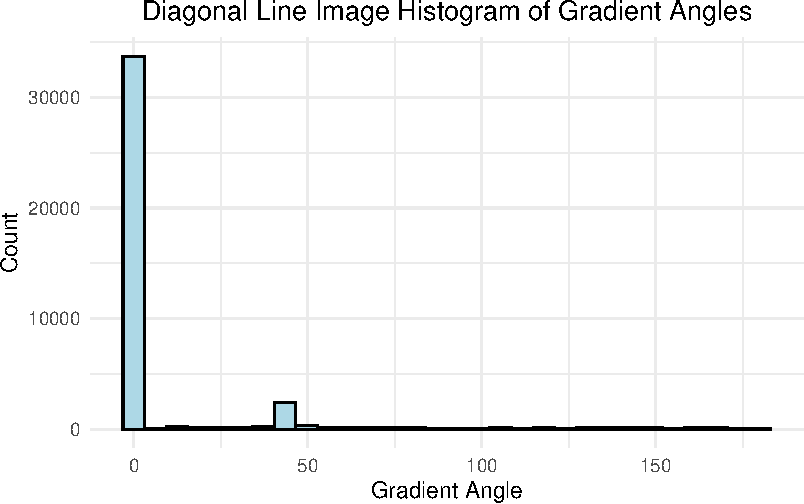
\includegraphics{results_files/figure-pdf/unnamed-chunk-9-6.pdf}

}

\end{figure}

\begin{Shaded}
\begin{Highlighting}[]
\FunctionTok{ggsave}\NormalTok{(}\StringTok{"images/plots/diagonal\_histogram\_theta\_plot.jpg"}\NormalTok{, diagonal\_histogram\_theta\_plot, }\AttributeTok{width =} \DecValTok{6}\NormalTok{, }\AttributeTok{height =} \DecValTok{4}\NormalTok{, }\AttributeTok{dpi =} \DecValTok{300}\NormalTok{)}
\end{Highlighting}
\end{Shaded}

\begin{verbatim}
`stat_bin()` using `bins = 30`. Pick better value with `binwidth`.
\end{verbatim}

\begin{Shaded}
\begin{Highlighting}[]
\NormalTok{sf\_histogram\_mag\_plot }\OtherTok{\textless{}{-}}
  \FunctionTok{ggplot}\NormalTok{(standard\_df\_list[[}\DecValTok{2}\NormalTok{]], }
         \FunctionTok{aes}\NormalTok{(}\AttributeTok{x =}\NormalTok{ mag)) }\SpecialCharTok{+}
  \FunctionTok{geom\_histogram}\NormalTok{(}\AttributeTok{colour =} \StringTok{"black"}\NormalTok{, }\AttributeTok{fill =} \StringTok{"lightblue"}\NormalTok{) }\SpecialCharTok{+}
  \FunctionTok{scale\_x\_continuous}\NormalTok{() }\SpecialCharTok{+} 
  \FunctionTok{labs}\NormalTok{(}\AttributeTok{x =} \StringTok{"Gradient Magnitude"}\NormalTok{, }
       \AttributeTok{y =} \StringTok{"Count"}\NormalTok{, }
       \AttributeTok{title =} \StringTok{"San Francisco Image Histogram of Gradient Magnitudes"}
\NormalTok{       ) }\SpecialCharTok{+}
  \FunctionTok{theme\_minimal}\NormalTok{() }\SpecialCharTok{+}
  \FunctionTok{theme}\NormalTok{(}\AttributeTok{plot.title =} \FunctionTok{element\_text}\NormalTok{(}\AttributeTok{hjust =} \FloatTok{0.5}\NormalTok{))}

\NormalTok{sf\_histogram\_mag\_plot}
\end{Highlighting}
\end{Shaded}

\begin{verbatim}
`stat_bin()` using `bins = 30`. Pick better value with `binwidth`.
\end{verbatim}

\begin{figure}[H]

{\centering 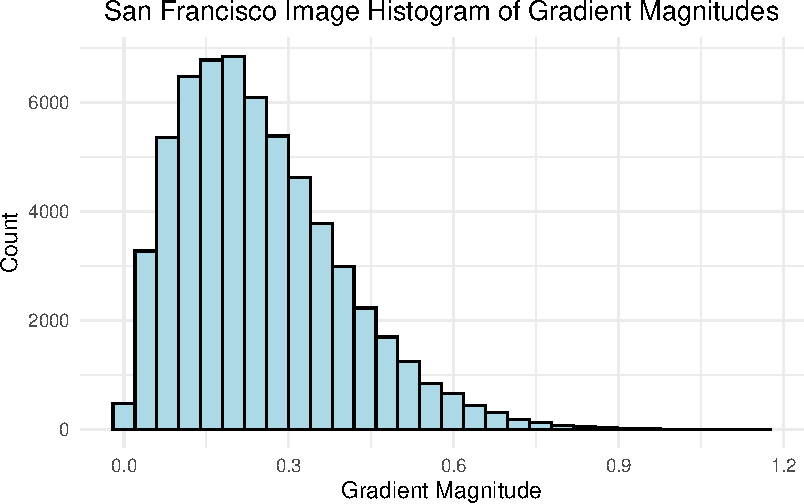
\includegraphics{results_files/figure-pdf/unnamed-chunk-10-1.pdf}

}

\end{figure}

\begin{Shaded}
\begin{Highlighting}[]
\NormalTok{sf\_mag\_filter }\OtherTok{\textless{}{-}} \FloatTok{0.4}

\FunctionTok{ggsave}\NormalTok{(}\StringTok{"images/plots/sf\_histogram\_mag\_plot.jpg"}\NormalTok{, sf\_histogram\_mag\_plot, }\AttributeTok{width =} \DecValTok{6}\NormalTok{, }\AttributeTok{height =} \DecValTok{4}\NormalTok{, }\AttributeTok{dpi =} \DecValTok{300}\NormalTok{)}
\end{Highlighting}
\end{Shaded}

\begin{verbatim}
`stat_bin()` using `bins = 30`. Pick better value with `binwidth`.
\end{verbatim}

\begin{Shaded}
\begin{Highlighting}[]
\NormalTok{sf\_histogram\_theta\_plot }\OtherTok{\textless{}{-}}
  \FunctionTok{ggplot}\NormalTok{(standard\_df\_list[[}\DecValTok{2}\NormalTok{]], }
         \FunctionTok{aes}\NormalTok{(}\AttributeTok{x =}\NormalTok{ theta)) }\SpecialCharTok{+}
  \FunctionTok{geom\_histogram}\NormalTok{(}\AttributeTok{colour =} \StringTok{"black"}\NormalTok{, }\AttributeTok{fill =} \StringTok{"lightblue"}\NormalTok{) }\SpecialCharTok{+}
  \FunctionTok{scale\_x\_continuous}\NormalTok{() }\SpecialCharTok{+} 
  \FunctionTok{labs}\NormalTok{(}\AttributeTok{x =} \StringTok{"Gradient Angle"}\NormalTok{, }
       \AttributeTok{y =} \StringTok{"Count"}\NormalTok{, }
       \AttributeTok{title =} \StringTok{"San Francisco Image Histogram of Gradient Angles"}
\NormalTok{       ) }\SpecialCharTok{+}
  \FunctionTok{theme\_minimal}\NormalTok{() }\SpecialCharTok{+}
  \FunctionTok{theme}\NormalTok{(}\AttributeTok{plot.title =} \FunctionTok{element\_text}\NormalTok{(}\AttributeTok{hjust =} \FloatTok{0.5}\NormalTok{))}

\NormalTok{sf\_histogram\_theta\_plot}
\end{Highlighting}
\end{Shaded}

\begin{verbatim}
`stat_bin()` using `bins = 30`. Pick better value with `binwidth`.
\end{verbatim}

\begin{figure}[H]

{\centering 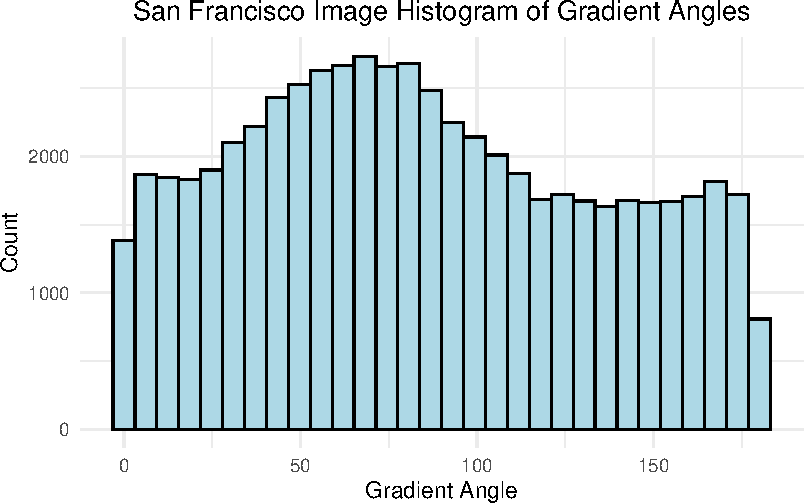
\includegraphics{results_files/figure-pdf/unnamed-chunk-10-2.pdf}

}

\end{figure}

\begin{Shaded}
\begin{Highlighting}[]
\FunctionTok{ggsave}\NormalTok{(}\StringTok{"images/plots/sf\_histogram\_theta\_plot.jpg"}\NormalTok{, sf\_histogram\_theta\_plot, }\AttributeTok{width =} \DecValTok{6}\NormalTok{, }\AttributeTok{height =} \DecValTok{4}\NormalTok{, }\AttributeTok{dpi =} \DecValTok{300}\NormalTok{)}
\end{Highlighting}
\end{Shaded}

\begin{verbatim}
`stat_bin()` using `bins = 30`. Pick better value with `binwidth`.
\end{verbatim}

\begin{Shaded}
\begin{Highlighting}[]
\NormalTok{internet\_grass\_histogram\_mag\_plot }\OtherTok{\textless{}{-}}
  \FunctionTok{ggplot}\NormalTok{(standard\_df\_list[[}\DecValTok{3}\NormalTok{]], }
         \FunctionTok{aes}\NormalTok{(}\AttributeTok{x =}\NormalTok{ mag)) }\SpecialCharTok{+}
  \FunctionTok{geom\_histogram}\NormalTok{(}\AttributeTok{colour =} \StringTok{"black"}\NormalTok{, }\AttributeTok{fill =} \StringTok{"lightblue"}\NormalTok{) }\SpecialCharTok{+}
  \FunctionTok{scale\_x\_continuous}\NormalTok{() }\SpecialCharTok{+} 
  \FunctionTok{labs}\NormalTok{(}\AttributeTok{x =} \StringTok{"Gradient Magnitude"}\NormalTok{, }
       \AttributeTok{y =} \StringTok{"Count"}\NormalTok{, }
       \AttributeTok{title =} \StringTok{"Internet Grass Image Histogram of Gradient Magnitudes"}
\NormalTok{       ) }\SpecialCharTok{+}
  \FunctionTok{theme\_minimal}\NormalTok{() }\SpecialCharTok{+}
  \FunctionTok{theme}\NormalTok{(}\AttributeTok{plot.title =} \FunctionTok{element\_text}\NormalTok{(}\AttributeTok{hjust =} \FloatTok{0.5}\NormalTok{))}

\NormalTok{internet\_grass\_histogram\_mag\_plot}
\end{Highlighting}
\end{Shaded}

\begin{verbatim}
`stat_bin()` using `bins = 30`. Pick better value with `binwidth`.
\end{verbatim}

\begin{figure}[H]

{\centering 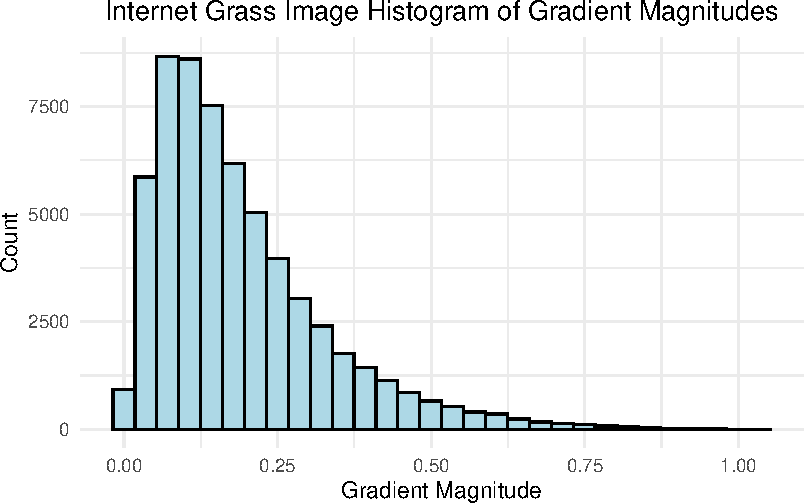
\includegraphics{results_files/figure-pdf/unnamed-chunk-11-1.pdf}

}

\end{figure}

\begin{Shaded}
\begin{Highlighting}[]
\NormalTok{internet\_grass\_mag\_filter }\OtherTok{\textless{}{-}} \FloatTok{0.3}

\FunctionTok{ggsave}\NormalTok{(}\StringTok{"images/plots/internet\_grass\_histogram\_mag\_plot.jpg"}\NormalTok{, internet\_grass\_histogram\_mag\_plot, }\AttributeTok{width =} \DecValTok{6}\NormalTok{, }\AttributeTok{height =} \DecValTok{4}\NormalTok{, }\AttributeTok{dpi =} \DecValTok{300}\NormalTok{)}
\end{Highlighting}
\end{Shaded}

\begin{verbatim}
`stat_bin()` using `bins = 30`. Pick better value with `binwidth`.
\end{verbatim}

\begin{Shaded}
\begin{Highlighting}[]
\NormalTok{internet\_grass\_histogram\_theta\_plot }\OtherTok{\textless{}{-}}
  \FunctionTok{ggplot}\NormalTok{(standard\_df\_list[[}\DecValTok{3}\NormalTok{]], }
         \FunctionTok{aes}\NormalTok{(}\AttributeTok{x =}\NormalTok{ theta)) }\SpecialCharTok{+}
  \FunctionTok{geom\_histogram}\NormalTok{(}\AttributeTok{colour =} \StringTok{"black"}\NormalTok{, }\AttributeTok{fill =} \StringTok{"lightblue"}\NormalTok{) }\SpecialCharTok{+}
  \FunctionTok{scale\_x\_continuous}\NormalTok{() }\SpecialCharTok{+} 
  \FunctionTok{labs}\NormalTok{(}\AttributeTok{x =} \StringTok{"Gradient Angle"}\NormalTok{, }
       \AttributeTok{y =} \StringTok{"Count"}\NormalTok{, }
       \AttributeTok{title =} \StringTok{"Internet Grass Image Histogram of Gradient Angles"}
\NormalTok{       ) }\SpecialCharTok{+}
  \FunctionTok{theme\_minimal}\NormalTok{() }\SpecialCharTok{+}
  \FunctionTok{theme}\NormalTok{(}\AttributeTok{plot.title =} \FunctionTok{element\_text}\NormalTok{(}\AttributeTok{hjust =} \FloatTok{0.5}\NormalTok{))}

\NormalTok{internet\_grass\_histogram\_theta\_plot}
\end{Highlighting}
\end{Shaded}

\begin{verbatim}
`stat_bin()` using `bins = 30`. Pick better value with `binwidth`.
\end{verbatim}

\begin{figure}[H]

{\centering 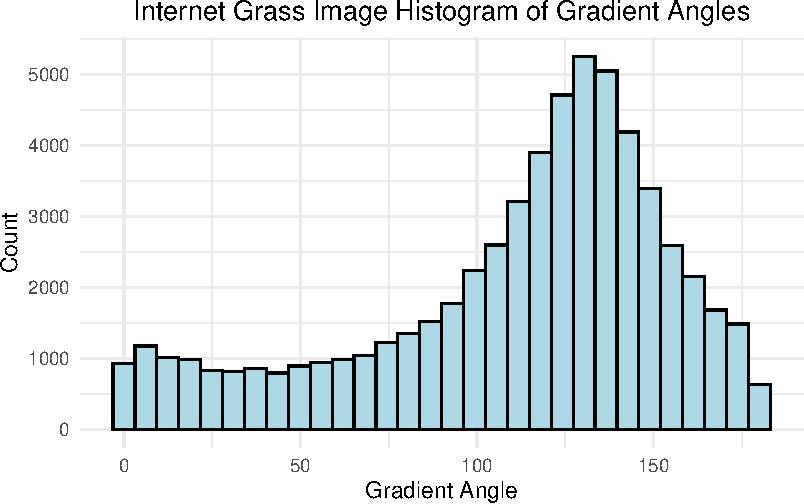
\includegraphics{results_files/figure-pdf/unnamed-chunk-11-2.pdf}

}

\end{figure}

\begin{Shaded}
\begin{Highlighting}[]
\FunctionTok{ggsave}\NormalTok{(}\StringTok{"images/plots/internet\_grass\_histogram\_theta\_plot.jpg"}\NormalTok{, internet\_grass\_histogram\_theta\_plot, }\AttributeTok{width =} \DecValTok{6}\NormalTok{, }\AttributeTok{height =} \DecValTok{4}\NormalTok{, }\AttributeTok{dpi =} \DecValTok{300}\NormalTok{)}
\end{Highlighting}
\end{Shaded}

\begin{verbatim}
`stat_bin()` using `bins = 30`. Pick better value with `binwidth`.
\end{verbatim}

\begin{Shaded}
\begin{Highlighting}[]
\NormalTok{living\_labs\_histogram\_mag\_plot }\OtherTok{\textless{}{-}}
  \FunctionTok{ggplot}\NormalTok{(standard\_df\_list[[}\DecValTok{4}\NormalTok{]], }
         \FunctionTok{aes}\NormalTok{(}\AttributeTok{x =}\NormalTok{ mag)) }\SpecialCharTok{+}
  \FunctionTok{geom\_histogram}\NormalTok{(}\AttributeTok{colour =} \StringTok{"black"}\NormalTok{, }\AttributeTok{fill =} \StringTok{"lightblue"}\NormalTok{) }\SpecialCharTok{+}
  \FunctionTok{scale\_x\_continuous}\NormalTok{() }\SpecialCharTok{+} 
  \FunctionTok{labs}\NormalTok{(}\AttributeTok{x =} \StringTok{"Gradient Magnitude"}\NormalTok{, }
       \AttributeTok{y =} \StringTok{"Count"}\NormalTok{, }
       \AttributeTok{title =} \StringTok{"Living Labs Grass Image Histogram of Gradient Magnitudes"}
\NormalTok{       ) }\SpecialCharTok{+}
  \FunctionTok{theme\_minimal}\NormalTok{() }\SpecialCharTok{+}
  \FunctionTok{theme}\NormalTok{(}\AttributeTok{plot.title =} \FunctionTok{element\_text}\NormalTok{(}\AttributeTok{hjust =} \FloatTok{0.5}\NormalTok{))}

\NormalTok{living\_labs\_histogram\_mag\_plot}
\end{Highlighting}
\end{Shaded}

\begin{verbatim}
`stat_bin()` using `bins = 30`. Pick better value with `binwidth`.
\end{verbatim}

\begin{figure}[H]

{\centering 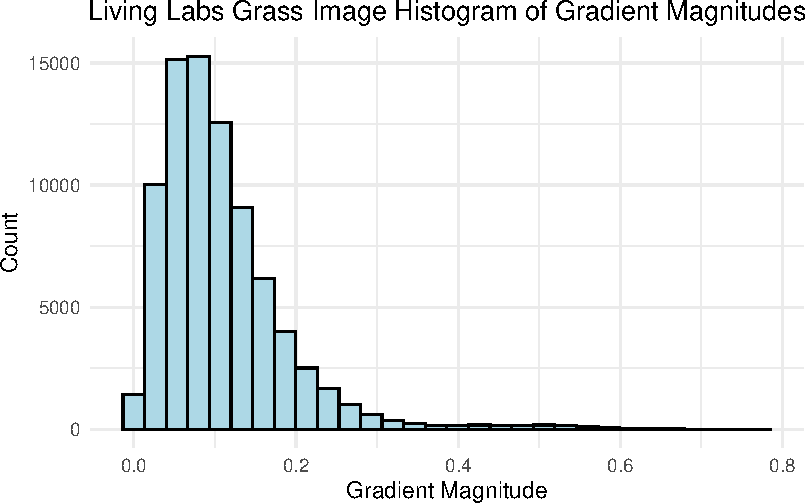
\includegraphics{results_files/figure-pdf/unnamed-chunk-12-1.pdf}

}

\end{figure}

\begin{Shaded}
\begin{Highlighting}[]
\NormalTok{living\_labs\_\_mag\_filter }\OtherTok{\textless{}{-}} \FloatTok{0.15}

\FunctionTok{ggsave}\NormalTok{(}\StringTok{"images/plots/living\_labs\_histogram\_mag\_plot.jpg"}\NormalTok{, living\_labs\_histogram\_mag\_plot, }\AttributeTok{width =} \DecValTok{6}\NormalTok{, }\AttributeTok{height =} \DecValTok{4}\NormalTok{, }\AttributeTok{dpi =} \DecValTok{300}\NormalTok{)}
\end{Highlighting}
\end{Shaded}

\begin{verbatim}
`stat_bin()` using `bins = 30`. Pick better value with `binwidth`.
\end{verbatim}

\begin{Shaded}
\begin{Highlighting}[]
\NormalTok{living\_labs\_histogram\_theta\_plot }\OtherTok{\textless{}{-}}
  \FunctionTok{ggplot}\NormalTok{(standard\_df\_list[[}\DecValTok{4}\NormalTok{]], }
         \FunctionTok{aes}\NormalTok{(}\AttributeTok{x =}\NormalTok{ theta)) }\SpecialCharTok{+}
  \FunctionTok{geom\_histogram}\NormalTok{(}\AttributeTok{colour =} \StringTok{"black"}\NormalTok{, }\AttributeTok{fill =} \StringTok{"lightblue"}\NormalTok{) }\SpecialCharTok{+}
  \FunctionTok{scale\_x\_continuous}\NormalTok{() }\SpecialCharTok{+} 
  \FunctionTok{labs}\NormalTok{(}\AttributeTok{x =} \StringTok{"Gradient Angle"}\NormalTok{, }
       \AttributeTok{y =} \StringTok{"Count"}\NormalTok{, }
       \AttributeTok{title =} \StringTok{"Living Labs Grass Image Histogram of Gradient Angles"}
\NormalTok{       ) }\SpecialCharTok{+}
  \FunctionTok{theme\_minimal}\NormalTok{() }\SpecialCharTok{+}
  \FunctionTok{theme}\NormalTok{(}\AttributeTok{plot.title =} \FunctionTok{element\_text}\NormalTok{(}\AttributeTok{hjust =} \FloatTok{0.5}\NormalTok{))}

\NormalTok{living\_labs\_histogram\_theta\_plot}
\end{Highlighting}
\end{Shaded}

\begin{verbatim}
`stat_bin()` using `bins = 30`. Pick better value with `binwidth`.
\end{verbatim}

\begin{figure}[H]

{\centering 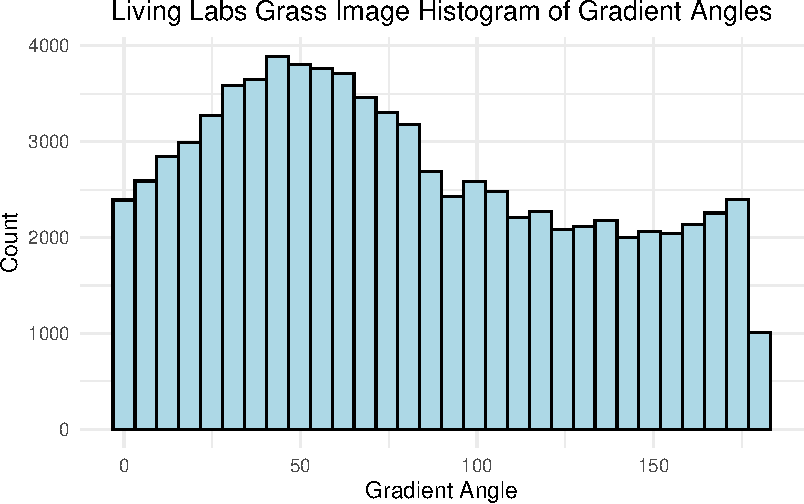
\includegraphics{results_files/figure-pdf/unnamed-chunk-12-2.pdf}

}

\end{figure}

\begin{Shaded}
\begin{Highlighting}[]
\FunctionTok{ggsave}\NormalTok{(}\StringTok{"images/plots/living\_labs\_histogram\_theta\_plot.jpg"}\NormalTok{, living\_labs\_histogram\_theta\_plot, }\AttributeTok{width =} \DecValTok{6}\NormalTok{, }\AttributeTok{height =} \DecValTok{4}\NormalTok{, }\AttributeTok{dpi =} \DecValTok{300}\NormalTok{)}
\end{Highlighting}
\end{Shaded}

\begin{verbatim}
`stat_bin()` using `bins = 30`. Pick better value with `binwidth`.
\end{verbatim}

\hypertarget{build-new-contribution-histograms-for-each-data-frame}{%
\section{Build New Contribution Histograms for Each Data
Frame}\label{build-new-contribution-histograms-for-each-data-frame}}

\begin{Shaded}
\begin{Highlighting}[]
\CommentTok{\# Define the number of bins}
\NormalTok{num\_bins }\OtherTok{\textless{}{-}} \DecValTok{9}

\CommentTok{\# function to calculate the contributions to neighboring bins}
\NormalTok{calculate\_bin\_contributions }\OtherTok{\textless{}{-}} \ControlFlowTok{function}\NormalTok{(angle, magnitude, num\_bins) \{}
\NormalTok{  bin\_width }\OtherTok{\textless{}{-}} \DecValTok{180} \SpecialCharTok{/}\NormalTok{ num\_bins}
\NormalTok{  contributions }\OtherTok{\textless{}{-}} \FunctionTok{numeric}\NormalTok{(num\_bins)}
  
  \CommentTok{\# get the central bin}
\NormalTok{  central\_bin }\OtherTok{\textless{}{-}} \FunctionTok{floor}\NormalTok{(angle }\SpecialCharTok{/}\NormalTok{ bin\_width) }\SpecialCharTok{\%\%}\NormalTok{ num\_bins}
\NormalTok{  next\_bin }\OtherTok{\textless{}{-}}\NormalTok{ (central\_bin }\SpecialCharTok{+} \DecValTok{1}\NormalTok{) }\SpecialCharTok{\%\%}\NormalTok{ num\_bins}
  
  \CommentTok{\# get contributions to neighboring bins}
\NormalTok{  weight }\OtherTok{\textless{}{-}}\NormalTok{ (}\DecValTok{1} \SpecialCharTok{{-}} \FunctionTok{abs}\NormalTok{((angle }\SpecialCharTok{\%\%}\NormalTok{ bin\_width) }\SpecialCharTok{/}\NormalTok{ bin\_width)) }\SpecialCharTok{*}\NormalTok{ magnitude}
  
\NormalTok{  contributions[central\_bin }\SpecialCharTok{+} \DecValTok{1}\NormalTok{] }\OtherTok{\textless{}{-}}\NormalTok{ weight}
\NormalTok{  contributions[next\_bin }\SpecialCharTok{+} \DecValTok{1}\NormalTok{] }\OtherTok{\textless{}{-}}\NormalTok{ magnitude }\SpecialCharTok{{-}}\NormalTok{ weight}
  
  \FunctionTok{return}\NormalTok{(}\FunctionTok{list}\NormalTok{(contributions[}\DecValTok{1}\NormalTok{],}
\NormalTok{         contributions[}\DecValTok{2}\NormalTok{],}
\NormalTok{         contributions[}\DecValTok{3}\NormalTok{],}
\NormalTok{         contributions[}\DecValTok{4}\NormalTok{],}
\NormalTok{         contributions[}\DecValTok{5}\NormalTok{],}
\NormalTok{         contributions[}\DecValTok{6}\NormalTok{],}
\NormalTok{         contributions[}\DecValTok{7}\NormalTok{],}
\NormalTok{         contributions[}\DecValTok{8}\NormalTok{],}
\NormalTok{         contributions[}\DecValTok{9}\NormalTok{])}
\NormalTok{         )}
\NormalTok{\}}

\NormalTok{filtered\_standard\_df\_list }\OtherTok{\textless{}{-}}\FunctionTok{list}\NormalTok{(diagonal\_hog\_df }\SpecialCharTok{\%\textgreater{}\%}
                                   \FunctionTok{filter}\NormalTok{(mag }\SpecialCharTok{\textgreater{}=}\NormalTok{ diagonal\_mag\_filter),}
\NormalTok{                                 sf\_hog\_df }\SpecialCharTok{\%\textgreater{}\%}
                                   \FunctionTok{filter}\NormalTok{(mag }\SpecialCharTok{\textgreater{}=}\NormalTok{ sf\_mag\_filter), }
\NormalTok{                                 internet\_grass\_hog\_df }\SpecialCharTok{\%\textgreater{}\%}
                                   \FunctionTok{filter}\NormalTok{(mag }\SpecialCharTok{\textgreater{}=}\NormalTok{ internet\_grass\_mag\_filter), }
\NormalTok{                                 living\_labs\_hog\_df }\SpecialCharTok{\%\textgreater{}\%}
                                   \FunctionTok{filter}\NormalTok{(mag }\SpecialCharTok{\textgreater{}=}\NormalTok{ living\_labs\_\_mag\_filter))}
\NormalTok{contribution\_df\_list }\OtherTok{\textless{}{-}} \FunctionTok{list}\NormalTok{()}

 
\ControlFlowTok{for}\NormalTok{ (i }\ControlFlowTok{in} \DecValTok{1}\SpecialCharTok{:}\FunctionTok{length}\NormalTok{(filtered\_standard\_df\_list))\{}
  
\NormalTok{  contribution\_hog\_df }\OtherTok{\textless{}{-}} 
\NormalTok{    filtered\_standard\_df\_list[[i]] }\SpecialCharTok{\%\textgreater{}\%}
    \FunctionTok{filter}\NormalTok{(mag }\SpecialCharTok{\textgreater{}} \FloatTok{0.1}\NormalTok{) }\SpecialCharTok{\%\textgreater{}\%}
    \FunctionTok{rowwise}\NormalTok{() }\SpecialCharTok{\%\textgreater{}\%}
    \FunctionTok{mutate}\NormalTok{(}\StringTok{\textasciigrave{}}\AttributeTok{0}\StringTok{\textasciigrave{}} \OtherTok{=} \FunctionTok{calculate\_bin\_contributions}\NormalTok{(theta, mag, }\DecValTok{9}\NormalTok{)[[}\DecValTok{1}\NormalTok{]],}
           \StringTok{\textasciigrave{}}\AttributeTok{20}\StringTok{\textasciigrave{}} \OtherTok{=} \FunctionTok{calculate\_bin\_contributions}\NormalTok{(theta, mag, }\DecValTok{9}\NormalTok{)[[}\DecValTok{2}\NormalTok{]],}
           \StringTok{\textasciigrave{}}\AttributeTok{40}\StringTok{\textasciigrave{}} \OtherTok{=} \FunctionTok{calculate\_bin\_contributions}\NormalTok{(theta, mag, }\DecValTok{9}\NormalTok{)[[}\DecValTok{3}\NormalTok{]],}
           \StringTok{\textasciigrave{}}\AttributeTok{60}\StringTok{\textasciigrave{}} \OtherTok{=} \FunctionTok{calculate\_bin\_contributions}\NormalTok{(theta, mag, }\DecValTok{9}\NormalTok{)[[}\DecValTok{4}\NormalTok{]],}
           \StringTok{\textasciigrave{}}\AttributeTok{80}\StringTok{\textasciigrave{}} \OtherTok{=} \FunctionTok{calculate\_bin\_contributions}\NormalTok{(theta, mag, }\DecValTok{9}\NormalTok{)[[}\DecValTok{5}\NormalTok{]],}
           \StringTok{\textasciigrave{}}\AttributeTok{100}\StringTok{\textasciigrave{}} \OtherTok{=} \FunctionTok{calculate\_bin\_contributions}\NormalTok{(theta, mag, }\DecValTok{9}\NormalTok{)[[}\DecValTok{6}\NormalTok{]],}
           \StringTok{\textasciigrave{}}\AttributeTok{120}\StringTok{\textasciigrave{}} \OtherTok{=} \FunctionTok{calculate\_bin\_contributions}\NormalTok{(theta, mag, }\DecValTok{9}\NormalTok{)[[}\DecValTok{7}\NormalTok{]],}
           \StringTok{\textasciigrave{}}\AttributeTok{140}\StringTok{\textasciigrave{}} \OtherTok{=} \FunctionTok{calculate\_bin\_contributions}\NormalTok{(theta, mag, }\DecValTok{9}\NormalTok{)[[}\DecValTok{8}\NormalTok{]],}
           \StringTok{\textasciigrave{}}\AttributeTok{160}\StringTok{\textasciigrave{}} \OtherTok{=} \FunctionTok{calculate\_bin\_contributions}\NormalTok{(theta, mag, }\DecValTok{9}\NormalTok{)[[}\DecValTok{9}\NormalTok{]],}
\NormalTok{           )}
  
\NormalTok{  split\_histo\_df }\OtherTok{\textless{}{-}} 
\NormalTok{    contribution\_hog\_df }\SpecialCharTok{\%\textgreater{}\%}
    \FunctionTok{pivot\_longer}\NormalTok{(}\AttributeTok{names\_to =} \StringTok{"bin"}\NormalTok{, }
                 \AttributeTok{values\_to =} \StringTok{"contribution"}\NormalTok{, }
                 \AttributeTok{cols =} \DecValTok{4}\SpecialCharTok{:}\FunctionTok{ncol}\NormalTok{(contribution\_hog\_df)) }\SpecialCharTok{\%\textgreater{}\%}
    \FunctionTok{mutate}\NormalTok{(}\AttributeTok{bin =} \FunctionTok{as.numeric}\NormalTok{(bin)) }\SpecialCharTok{\%\textgreater{}\%}
    \FunctionTok{group\_by}\NormalTok{(bin) }\SpecialCharTok{\%\textgreater{}\%}
    \FunctionTok{summarise}\NormalTok{(}\AttributeTok{contribution\_sum =} \FunctionTok{sum}\NormalTok{(contribution))}
  
  
\NormalTok{  contribution\_df\_list[[i]] }\OtherTok{\textless{}{-}}\NormalTok{ split\_histo\_df}

\NormalTok{\}}
\end{Highlighting}
\end{Shaded}

\hypertarget{generate-polar-plots-for-standard-historgrams}{%
\section{Generate Polar Plots for Standard
Historgrams}\label{generate-polar-plots-for-standard-historgrams}}

\begin{Shaded}
\begin{Highlighting}[]
\NormalTok{diagonal\_plot }\OtherTok{\textless{}{-}}
  \FunctionTok{ggplot}\NormalTok{(filtered\_standard\_df\_list[[}\DecValTok{1}\NormalTok{]], }
         \FunctionTok{aes}\NormalTok{(}\AttributeTok{x =}\NormalTok{ theta)) }\SpecialCharTok{+}
  \FunctionTok{geom\_histogram}\NormalTok{(}\AttributeTok{colour =} \StringTok{"black"}\NormalTok{, }
                 \AttributeTok{fill =} \StringTok{"lightblue"}\NormalTok{, }
                 \AttributeTok{breaks =} \FunctionTok{seq}\NormalTok{(}\DecValTok{0}\NormalTok{, }\DecValTok{360}\NormalTok{, }\AttributeTok{length.out =} \FloatTok{17.5}\NormalTok{),}
                 \AttributeTok{bins =} \DecValTok{9}\NormalTok{) }\SpecialCharTok{+}
  \FunctionTok{coord\_polar}\NormalTok{(}
    \AttributeTok{theta =} \StringTok{"x"}\NormalTok{, }
    \AttributeTok{start =} \DecValTok{0}\NormalTok{, }
    \AttributeTok{direction =} \DecValTok{1}\NormalTok{) }\SpecialCharTok{+}
  \FunctionTok{scale\_x\_continuous}\NormalTok{(}\AttributeTok{limits =} \FunctionTok{c}\NormalTok{(}\DecValTok{0}\NormalTok{,}\DecValTok{360}\NormalTok{),}
    \AttributeTok{breaks =} \FunctionTok{c}\NormalTok{(}\DecValTok{0}\NormalTok{, }\DecValTok{45}\NormalTok{, }\DecValTok{90}\NormalTok{, }\DecValTok{135}\NormalTok{, }\DecValTok{180}\NormalTok{, }\DecValTok{225}\NormalTok{, }\DecValTok{270}\NormalTok{, }\DecValTok{315}\NormalTok{), }
    \AttributeTok{labels =} \FunctionTok{c}\NormalTok{(}\StringTok{"N"}\NormalTok{, }\StringTok{"NE"}\NormalTok{, }\StringTok{"E"}\NormalTok{, }\StringTok{"SE"}\NormalTok{, }\StringTok{"S"}\NormalTok{, }\StringTok{"SW"}\NormalTok{, }\StringTok{"W"}\NormalTok{, }\StringTok{"NW"}\NormalTok{)}
\NormalTok{  )}\SpecialCharTok{+}
  \FunctionTok{labs}\NormalTok{(}\AttributeTok{title =} \StringTok{"Polar Plot of Diagonal Line Image}\SpecialCharTok{\textbackslash{}n}\StringTok{Using Standard HOG Technique"}\NormalTok{) }\SpecialCharTok{+}
  \FunctionTok{theme\_minimal}\NormalTok{() }\SpecialCharTok{+}
  \FunctionTok{labs}\NormalTok{(}\AttributeTok{x =} \StringTok{""}\NormalTok{) }\SpecialCharTok{+}
  \FunctionTok{theme}\NormalTok{(}\AttributeTok{axis.title.y =} \FunctionTok{element\_blank}\NormalTok{(),}
        \AttributeTok{plot.title =} \FunctionTok{element\_text}\NormalTok{(}\AttributeTok{hjust =} \FloatTok{0.5}\NormalTok{))}

\CommentTok{\#diagonal\_plot}
\end{Highlighting}
\end{Shaded}

\begin{Shaded}
\begin{Highlighting}[]
\NormalTok{sf\_plot }\OtherTok{\textless{}{-}}
  \FunctionTok{ggplot}\NormalTok{(filtered\_standard\_df\_list[[}\DecValTok{2}\NormalTok{]], }
         \FunctionTok{aes}\NormalTok{(}\AttributeTok{x =}\NormalTok{ theta)) }\SpecialCharTok{+}
  \FunctionTok{geom\_histogram}\NormalTok{(}\AttributeTok{colour =} \StringTok{"black"}\NormalTok{, }
                 \AttributeTok{fill =} \StringTok{"lightblue"}\NormalTok{, }
                 \AttributeTok{breaks =} \FunctionTok{seq}\NormalTok{(}\DecValTok{0}\NormalTok{, }\DecValTok{360}\NormalTok{, }\AttributeTok{length.out =} \FloatTok{17.5}\NormalTok{),}
                 \AttributeTok{bins =} \DecValTok{9}\NormalTok{) }\SpecialCharTok{+}
  \FunctionTok{coord\_polar}\NormalTok{(}
    \AttributeTok{theta =} \StringTok{"x"}\NormalTok{, }
    \AttributeTok{start =} \DecValTok{0}\NormalTok{, }
    \AttributeTok{direction =} \DecValTok{1}\NormalTok{) }\SpecialCharTok{+}
  \FunctionTok{scale\_x\_continuous}\NormalTok{(}\AttributeTok{limits =} \FunctionTok{c}\NormalTok{(}\DecValTok{0}\NormalTok{,}\DecValTok{360}\NormalTok{),}
    \AttributeTok{breaks =} \FunctionTok{c}\NormalTok{(}\DecValTok{0}\NormalTok{, }\DecValTok{45}\NormalTok{, }\DecValTok{90}\NormalTok{, }\DecValTok{135}\NormalTok{, }\DecValTok{180}\NormalTok{, }\DecValTok{225}\NormalTok{, }\DecValTok{270}\NormalTok{, }\DecValTok{315}\NormalTok{), }
    \AttributeTok{labels =} \FunctionTok{c}\NormalTok{(}\StringTok{"N"}\NormalTok{, }\StringTok{"NE"}\NormalTok{, }\StringTok{"E"}\NormalTok{, }\StringTok{"SE"}\NormalTok{, }\StringTok{"S"}\NormalTok{, }\StringTok{"SW"}\NormalTok{, }\StringTok{"W"}\NormalTok{, }\StringTok{"NW"}\NormalTok{)}
\NormalTok{  )}\SpecialCharTok{+}
  \FunctionTok{labs}\NormalTok{(}\AttributeTok{title =} \StringTok{"Polar Plot of San Francisco Image}\SpecialCharTok{\textbackslash{}n}\StringTok{Using Standard HOG Technique"}\NormalTok{) }\SpecialCharTok{+}
  \FunctionTok{theme\_minimal}\NormalTok{() }\SpecialCharTok{+}
  \FunctionTok{labs}\NormalTok{(}\AttributeTok{x =} \StringTok{""}\NormalTok{) }\SpecialCharTok{+}
  \FunctionTok{theme}\NormalTok{(}\AttributeTok{axis.title.y =} \FunctionTok{element\_blank}\NormalTok{(),}
        \AttributeTok{plot.title =} \FunctionTok{element\_text}\NormalTok{(}\AttributeTok{hjust =} \FloatTok{0.5}\NormalTok{))}

\CommentTok{\#sf\_plot}
\end{Highlighting}
\end{Shaded}

\begin{Shaded}
\begin{Highlighting}[]
\NormalTok{internet\_grass\_plot }\OtherTok{\textless{}{-}}
  \FunctionTok{ggplot}\NormalTok{(filtered\_standard\_df\_list[[}\DecValTok{3}\NormalTok{]], }
         \FunctionTok{aes}\NormalTok{(}\AttributeTok{x =}\NormalTok{ theta)) }\SpecialCharTok{+}
  \FunctionTok{geom\_histogram}\NormalTok{(}\AttributeTok{colour =} \StringTok{"black"}\NormalTok{, }
                 \AttributeTok{fill =} \StringTok{"lightblue"}\NormalTok{, }
                 \AttributeTok{breaks =} \FunctionTok{seq}\NormalTok{(}\DecValTok{0}\NormalTok{, }\DecValTok{360}\NormalTok{, }\AttributeTok{length.out =} \FloatTok{17.5}\NormalTok{),}
                 \AttributeTok{bins =} \DecValTok{9}\NormalTok{) }\SpecialCharTok{+}
  \FunctionTok{coord\_polar}\NormalTok{(}
    \AttributeTok{theta =} \StringTok{"x"}\NormalTok{, }
    \AttributeTok{start =} \DecValTok{0}\NormalTok{, }
    \AttributeTok{direction =} \DecValTok{1}\NormalTok{) }\SpecialCharTok{+}
  \FunctionTok{scale\_x\_continuous}\NormalTok{(}\AttributeTok{limits =} \FunctionTok{c}\NormalTok{(}\DecValTok{0}\NormalTok{,}\DecValTok{360}\NormalTok{),}
    \AttributeTok{breaks =} \FunctionTok{c}\NormalTok{(}\DecValTok{0}\NormalTok{, }\DecValTok{45}\NormalTok{, }\DecValTok{90}\NormalTok{, }\DecValTok{135}\NormalTok{, }\DecValTok{180}\NormalTok{, }\DecValTok{225}\NormalTok{, }\DecValTok{270}\NormalTok{, }\DecValTok{315}\NormalTok{), }
    \AttributeTok{labels =} \FunctionTok{c}\NormalTok{(}\StringTok{"N"}\NormalTok{, }\StringTok{"NE"}\NormalTok{, }\StringTok{"E"}\NormalTok{, }\StringTok{"SE"}\NormalTok{, }\StringTok{"S"}\NormalTok{, }\StringTok{"SW"}\NormalTok{, }\StringTok{"W"}\NormalTok{, }\StringTok{"NW"}\NormalTok{)}
\NormalTok{  )}\SpecialCharTok{+}
  \FunctionTok{labs}\NormalTok{(}\AttributeTok{title =} \StringTok{"Polar Plot of Internet Grass Image}\SpecialCharTok{\textbackslash{}n}\StringTok{Using Standard HOG Technique"}\NormalTok{) }\SpecialCharTok{+}
  \FunctionTok{theme\_minimal}\NormalTok{() }\SpecialCharTok{+}
  \FunctionTok{labs}\NormalTok{(}\AttributeTok{x =} \StringTok{""}\NormalTok{) }\SpecialCharTok{+}
  \FunctionTok{theme}\NormalTok{(}\AttributeTok{axis.title.y =} \FunctionTok{element\_blank}\NormalTok{(),}
        \AttributeTok{plot.title =} \FunctionTok{element\_text}\NormalTok{(}\AttributeTok{hjust =} \FloatTok{0.5}\NormalTok{))}

\CommentTok{\#internet\_grass\_plot}
\end{Highlighting}
\end{Shaded}

\begin{Shaded}
\begin{Highlighting}[]
\NormalTok{living\_labs\_plot }\OtherTok{\textless{}{-}}
  \FunctionTok{ggplot}\NormalTok{(filtered\_standard\_df\_list[[}\DecValTok{4}\NormalTok{]], }
         \FunctionTok{aes}\NormalTok{(}\AttributeTok{x =}\NormalTok{ theta)) }\SpecialCharTok{+}
  \FunctionTok{geom\_histogram}\NormalTok{(}\AttributeTok{colour =} \StringTok{"black"}\NormalTok{, }
                 \AttributeTok{fill =} \StringTok{"lightblue"}\NormalTok{, }
                 \AttributeTok{breaks =} \FunctionTok{seq}\NormalTok{(}\DecValTok{0}\NormalTok{, }\DecValTok{360}\NormalTok{, }\AttributeTok{length.out =} \FloatTok{17.5}\NormalTok{),}
                 \AttributeTok{bins =} \DecValTok{9}\NormalTok{) }\SpecialCharTok{+}
  \FunctionTok{coord\_polar}\NormalTok{(}
    \AttributeTok{theta =} \StringTok{"x"}\NormalTok{, }
    \AttributeTok{start =} \DecValTok{0}\NormalTok{, }
    \AttributeTok{direction =} \DecValTok{1}\NormalTok{) }\SpecialCharTok{+}
  \FunctionTok{scale\_x\_continuous}\NormalTok{(}\AttributeTok{limits =} \FunctionTok{c}\NormalTok{(}\DecValTok{0}\NormalTok{,}\DecValTok{360}\NormalTok{),}
    \AttributeTok{breaks =} \FunctionTok{c}\NormalTok{(}\DecValTok{0}\NormalTok{, }\DecValTok{45}\NormalTok{, }\DecValTok{90}\NormalTok{, }\DecValTok{135}\NormalTok{, }\DecValTok{180}\NormalTok{, }\DecValTok{225}\NormalTok{, }\DecValTok{270}\NormalTok{, }\DecValTok{315}\NormalTok{), }
    \AttributeTok{labels =} \FunctionTok{c}\NormalTok{(}\StringTok{"N"}\NormalTok{, }\StringTok{"NE"}\NormalTok{, }\StringTok{"E"}\NormalTok{, }\StringTok{"SE"}\NormalTok{, }\StringTok{"S"}\NormalTok{, }\StringTok{"SW"}\NormalTok{, }\StringTok{"W"}\NormalTok{, }\StringTok{"NW"}\NormalTok{)}
\NormalTok{  )}\SpecialCharTok{+}
  \FunctionTok{labs}\NormalTok{(}\AttributeTok{title =} \StringTok{"Polar Plot of Living Labs Grass Image}\SpecialCharTok{\textbackslash{}n}\StringTok{Using Standard HOG Technique"}\NormalTok{) }\SpecialCharTok{+}
  \FunctionTok{theme\_minimal}\NormalTok{() }\SpecialCharTok{+}
  \FunctionTok{labs}\NormalTok{(}\AttributeTok{x =} \StringTok{""}\NormalTok{) }\SpecialCharTok{+}
  \FunctionTok{theme}\NormalTok{(}\AttributeTok{axis.title.y =} \FunctionTok{element\_blank}\NormalTok{(),}
        \AttributeTok{plot.title =} \FunctionTok{element\_text}\NormalTok{(}\AttributeTok{hjust =} \FloatTok{0.5}\NormalTok{))}

\CommentTok{\#living\_labs\_plot}
\end{Highlighting}
\end{Shaded}

\begin{Shaded}
\begin{Highlighting}[]
\NormalTok{all\_standard\_plots }\OtherTok{\textless{}{-}}\NormalTok{ ggpubr}\SpecialCharTok{::}\FunctionTok{ggarrange}\NormalTok{(diagonal\_plot, }
\NormalTok{                                        sf\_plot, }
\NormalTok{                                        internet\_grass\_plot, }
\NormalTok{                                        living\_labs\_plot)}

\FunctionTok{ggsave}\NormalTok{(}\StringTok{"images/plots/all\_standard\_polar\_plots.jpg"}\NormalTok{, }
\NormalTok{       all\_standard\_plots, }\AttributeTok{width =} \DecValTok{7}\NormalTok{, }
       \AttributeTok{height =} \DecValTok{7}\NormalTok{)}

\NormalTok{all\_standard\_plots}
\end{Highlighting}
\end{Shaded}

\begin{figure}[H]

{\centering 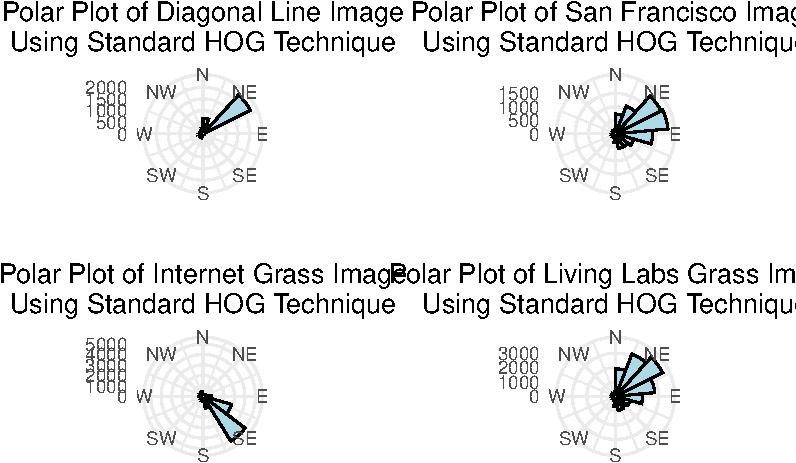
\includegraphics{results_files/figure-pdf/unnamed-chunk-18-1.pdf}

}

\end{figure}

\hypertarget{generate-polar-plots-for-contribution-historgrams}{%
\section{Generate Polar Plots for Contribution
Historgrams}\label{generate-polar-plots-for-contribution-historgrams}}

\begin{Shaded}
\begin{Highlighting}[]
\NormalTok{diagonal\_split\_plot }\OtherTok{\textless{}{-}}
  \FunctionTok{ggplot}\NormalTok{(contribution\_df\_list[[}\DecValTok{1}\NormalTok{]], }
         \FunctionTok{aes}\NormalTok{(}\AttributeTok{x =}\NormalTok{ bin, }\AttributeTok{y =}\NormalTok{ contribution\_sum)) }\SpecialCharTok{+}
  \FunctionTok{geom\_histogram}\NormalTok{(}\AttributeTok{stat =} \StringTok{"identity"}\NormalTok{,}
                 \AttributeTok{colour =} \StringTok{"black"}\NormalTok{, }
                 \AttributeTok{fill =} \StringTok{"lightblue"}\NormalTok{, }
                 \AttributeTok{breaks =} \FunctionTok{seq}\NormalTok{(}\DecValTok{0}\NormalTok{, }\DecValTok{360}\NormalTok{, }\AttributeTok{length.out =} \FloatTok{17.5}\NormalTok{),}
                 \AttributeTok{bins =} \DecValTok{9}\NormalTok{) }\SpecialCharTok{+}
  \FunctionTok{coord\_polar}\NormalTok{(}
    \AttributeTok{theta =} \StringTok{"x"}\NormalTok{, }
    \AttributeTok{start =} \DecValTok{0}\NormalTok{, }
    \AttributeTok{direction =} \DecValTok{1}\NormalTok{) }\SpecialCharTok{+}
  \FunctionTok{scale\_x\_continuous}\NormalTok{(}\AttributeTok{limits =} \FunctionTok{c}\NormalTok{(}\DecValTok{0}\NormalTok{,}\DecValTok{360}\NormalTok{),}
    \AttributeTok{breaks =} \FunctionTok{c}\NormalTok{(}\DecValTok{0}\NormalTok{, }\DecValTok{45}\NormalTok{, }\DecValTok{90}\NormalTok{, }\DecValTok{135}\NormalTok{, }\DecValTok{180}\NormalTok{, }\DecValTok{225}\NormalTok{, }\DecValTok{270}\NormalTok{, }\DecValTok{315}\NormalTok{), }
    \AttributeTok{labels =} \FunctionTok{c}\NormalTok{(}\StringTok{"N"}\NormalTok{, }\StringTok{"NE"}\NormalTok{, }\StringTok{"E"}\NormalTok{, }\StringTok{"SE"}\NormalTok{, }\StringTok{"S"}\NormalTok{, }\StringTok{"SW"}\NormalTok{, }\StringTok{"W"}\NormalTok{, }\StringTok{"NW"}\NormalTok{)}
\NormalTok{  )}\SpecialCharTok{+}
  \FunctionTok{labs}\NormalTok{(}\AttributeTok{title =} \StringTok{"Polar Plot of Diagonal Line Image}\SpecialCharTok{\textbackslash{}n}\StringTok{Using Distributed HOG Technique"}\NormalTok{) }\SpecialCharTok{+}
  \FunctionTok{theme\_minimal}\NormalTok{() }\SpecialCharTok{+}
  \FunctionTok{labs}\NormalTok{(}\AttributeTok{x =} \StringTok{""}\NormalTok{) }\SpecialCharTok{+}
  \FunctionTok{theme}\NormalTok{(}\AttributeTok{axis.title.y =} \FunctionTok{element\_blank}\NormalTok{(),}
        \AttributeTok{plot.title =} \FunctionTok{element\_text}\NormalTok{(}\AttributeTok{hjust =} \FloatTok{0.5}\NormalTok{))}
\end{Highlighting}
\end{Shaded}

\begin{verbatim}
Warning in geom_histogram(stat = "identity", colour = "black", fill =
"lightblue", : Ignoring unknown parameters: `binwidth`, `bins`, `pad`, and
`breaks`
\end{verbatim}

\begin{Shaded}
\begin{Highlighting}[]
\CommentTok{\#diagonal\_split\_plot}
\end{Highlighting}
\end{Shaded}

\begin{Shaded}
\begin{Highlighting}[]
\NormalTok{sf\_split\_plot }\OtherTok{\textless{}{-}}
  \FunctionTok{ggplot}\NormalTok{(contribution\_df\_list[[}\DecValTok{2}\NormalTok{]], }
         \FunctionTok{aes}\NormalTok{(}\AttributeTok{x =}\NormalTok{ bin, }\AttributeTok{y =}\NormalTok{ contribution\_sum)) }\SpecialCharTok{+}
  \FunctionTok{geom\_histogram}\NormalTok{(}\AttributeTok{stat =} \StringTok{"identity"}\NormalTok{,}
                 \AttributeTok{colour =} \StringTok{"black"}\NormalTok{, }
                 \AttributeTok{fill =} \StringTok{"lightblue"}\NormalTok{, }
                 \AttributeTok{breaks =} \FunctionTok{seq}\NormalTok{(}\DecValTok{0}\NormalTok{, }\DecValTok{360}\NormalTok{, }\AttributeTok{length.out =} \FloatTok{17.5}\NormalTok{),}
                 \AttributeTok{bins =} \DecValTok{9}\NormalTok{) }\SpecialCharTok{+}
  \FunctionTok{coord\_polar}\NormalTok{(}
    \AttributeTok{theta =} \StringTok{"x"}\NormalTok{, }
    \AttributeTok{start =} \DecValTok{0}\NormalTok{, }
    \AttributeTok{direction =} \DecValTok{1}\NormalTok{) }\SpecialCharTok{+}
  \FunctionTok{scale\_x\_continuous}\NormalTok{(}\AttributeTok{limits =} \FunctionTok{c}\NormalTok{(}\DecValTok{0}\NormalTok{,}\DecValTok{360}\NormalTok{),}
    \AttributeTok{breaks =} \FunctionTok{c}\NormalTok{(}\DecValTok{0}\NormalTok{, }\DecValTok{45}\NormalTok{, }\DecValTok{90}\NormalTok{, }\DecValTok{135}\NormalTok{, }\DecValTok{180}\NormalTok{, }\DecValTok{225}\NormalTok{, }\DecValTok{270}\NormalTok{, }\DecValTok{315}\NormalTok{), }
    \AttributeTok{labels =} \FunctionTok{c}\NormalTok{(}\StringTok{"N"}\NormalTok{, }\StringTok{"NE"}\NormalTok{, }\StringTok{"E"}\NormalTok{, }\StringTok{"SE"}\NormalTok{, }\StringTok{"S"}\NormalTok{, }\StringTok{"SW"}\NormalTok{, }\StringTok{"W"}\NormalTok{, }\StringTok{"NW"}\NormalTok{)}
\NormalTok{  )}\SpecialCharTok{+}
  \FunctionTok{labs}\NormalTok{(}\AttributeTok{title =} \StringTok{"Polar Plot of San Francisco Image}\SpecialCharTok{\textbackslash{}n}\StringTok{Using Distributed HOG Technique"}\NormalTok{) }\SpecialCharTok{+}
  \FunctionTok{theme\_minimal}\NormalTok{() }\SpecialCharTok{+}
  \FunctionTok{labs}\NormalTok{(}\AttributeTok{x =} \StringTok{""}\NormalTok{) }\SpecialCharTok{+}
  \FunctionTok{theme}\NormalTok{(}\AttributeTok{axis.title.y =} \FunctionTok{element\_blank}\NormalTok{(),}
        \AttributeTok{plot.title =} \FunctionTok{element\_text}\NormalTok{(}\AttributeTok{hjust =} \FloatTok{0.5}\NormalTok{))}
\end{Highlighting}
\end{Shaded}

\begin{verbatim}
Warning in geom_histogram(stat = "identity", colour = "black", fill =
"lightblue", : Ignoring unknown parameters: `binwidth`, `bins`, `pad`, and
`breaks`
\end{verbatim}

\begin{Shaded}
\begin{Highlighting}[]
\CommentTok{\#sf\_split\_plot}
\end{Highlighting}
\end{Shaded}

\begin{Shaded}
\begin{Highlighting}[]
\NormalTok{internet\_grass\_split\_plot }\OtherTok{\textless{}{-}}
  \FunctionTok{ggplot}\NormalTok{(contribution\_df\_list[[}\DecValTok{3}\NormalTok{]], }
         \FunctionTok{aes}\NormalTok{(}\AttributeTok{x =}\NormalTok{ bin, }\AttributeTok{y =}\NormalTok{ contribution\_sum)) }\SpecialCharTok{+}
  \FunctionTok{geom\_histogram}\NormalTok{(}\AttributeTok{stat =} \StringTok{"identity"}\NormalTok{,}
                 \AttributeTok{colour =} \StringTok{"black"}\NormalTok{, }
                 \AttributeTok{fill =} \StringTok{"lightblue"}\NormalTok{, }
                 \AttributeTok{breaks =} \FunctionTok{seq}\NormalTok{(}\DecValTok{0}\NormalTok{, }\DecValTok{360}\NormalTok{, }\AttributeTok{length.out =} \FloatTok{17.5}\NormalTok{),}
                 \AttributeTok{bins =} \DecValTok{9}\NormalTok{) }\SpecialCharTok{+}
  \FunctionTok{coord\_polar}\NormalTok{(}
    \AttributeTok{theta =} \StringTok{"x"}\NormalTok{, }
    \AttributeTok{start =} \DecValTok{0}\NormalTok{, }
    \AttributeTok{direction =} \DecValTok{1}\NormalTok{) }\SpecialCharTok{+}
  \FunctionTok{scale\_x\_continuous}\NormalTok{(}\AttributeTok{limits =} \FunctionTok{c}\NormalTok{(}\DecValTok{0}\NormalTok{,}\DecValTok{360}\NormalTok{),}
    \AttributeTok{breaks =} \FunctionTok{c}\NormalTok{(}\DecValTok{0}\NormalTok{, }\DecValTok{45}\NormalTok{, }\DecValTok{90}\NormalTok{, }\DecValTok{135}\NormalTok{, }\DecValTok{180}\NormalTok{, }\DecValTok{225}\NormalTok{, }\DecValTok{270}\NormalTok{, }\DecValTok{315}\NormalTok{), }
    \AttributeTok{labels =} \FunctionTok{c}\NormalTok{(}\StringTok{"N"}\NormalTok{, }\StringTok{"NE"}\NormalTok{, }\StringTok{"E"}\NormalTok{, }\StringTok{"SE"}\NormalTok{, }\StringTok{"S"}\NormalTok{, }\StringTok{"SW"}\NormalTok{, }\StringTok{"W"}\NormalTok{, }\StringTok{"NW"}\NormalTok{)}
\NormalTok{  )}\SpecialCharTok{+}
  \FunctionTok{labs}\NormalTok{(}\AttributeTok{title =} \StringTok{"Polar Plot of Internet Grass Image}\SpecialCharTok{\textbackslash{}n}\StringTok{Using Distributed HOG Technique"}\NormalTok{) }\SpecialCharTok{+}
  \FunctionTok{theme\_minimal}\NormalTok{() }\SpecialCharTok{+}
  \FunctionTok{labs}\NormalTok{(}\AttributeTok{x =} \StringTok{""}\NormalTok{) }\SpecialCharTok{+}
  \FunctionTok{theme}\NormalTok{(}\AttributeTok{axis.title.y =} \FunctionTok{element\_blank}\NormalTok{(),}
        \AttributeTok{plot.title =} \FunctionTok{element\_text}\NormalTok{(}\AttributeTok{hjust =} \FloatTok{0.5}\NormalTok{))}
\end{Highlighting}
\end{Shaded}

\begin{verbatim}
Warning in geom_histogram(stat = "identity", colour = "black", fill =
"lightblue", : Ignoring unknown parameters: `binwidth`, `bins`, `pad`, and
`breaks`
\end{verbatim}

\begin{Shaded}
\begin{Highlighting}[]
\CommentTok{\#internet\_grass\_split\_plot}
\end{Highlighting}
\end{Shaded}

\begin{Shaded}
\begin{Highlighting}[]
\NormalTok{living\_labs\_split\_plot }\OtherTok{\textless{}{-}}
  \FunctionTok{ggplot}\NormalTok{(contribution\_df\_list[[}\DecValTok{4}\NormalTok{]], }
         \FunctionTok{aes}\NormalTok{(}\AttributeTok{x =}\NormalTok{ bin, }\AttributeTok{y =}\NormalTok{ contribution\_sum)) }\SpecialCharTok{+}
  \FunctionTok{geom\_histogram}\NormalTok{(}\AttributeTok{stat =} \StringTok{"identity"}\NormalTok{,}
                 \AttributeTok{colour =} \StringTok{"black"}\NormalTok{, }
                 \AttributeTok{fill =} \StringTok{"lightblue"}\NormalTok{, }
                 \AttributeTok{breaks =} \FunctionTok{seq}\NormalTok{(}\DecValTok{0}\NormalTok{, }\DecValTok{360}\NormalTok{, }\AttributeTok{length.out =} \FloatTok{17.5}\NormalTok{),}
                 \AttributeTok{bins =} \DecValTok{9}\NormalTok{) }\SpecialCharTok{+}
  \FunctionTok{coord\_polar}\NormalTok{(}
    \AttributeTok{theta =} \StringTok{"x"}\NormalTok{, }
    \AttributeTok{start =} \DecValTok{0}\NormalTok{, }
    \AttributeTok{direction =} \DecValTok{1}\NormalTok{) }\SpecialCharTok{+}
  \FunctionTok{scale\_x\_continuous}\NormalTok{(}\AttributeTok{limits =} \FunctionTok{c}\NormalTok{(}\DecValTok{0}\NormalTok{,}\DecValTok{360}\NormalTok{),}
    \AttributeTok{breaks =} \FunctionTok{c}\NormalTok{(}\DecValTok{0}\NormalTok{, }\DecValTok{45}\NormalTok{, }\DecValTok{90}\NormalTok{, }\DecValTok{135}\NormalTok{, }\DecValTok{180}\NormalTok{, }\DecValTok{225}\NormalTok{, }\DecValTok{270}\NormalTok{, }\DecValTok{315}\NormalTok{), }
    \AttributeTok{labels =} \FunctionTok{c}\NormalTok{(}\StringTok{"N"}\NormalTok{, }\StringTok{"NE"}\NormalTok{, }\StringTok{"E"}\NormalTok{, }\StringTok{"SE"}\NormalTok{, }\StringTok{"S"}\NormalTok{, }\StringTok{"SW"}\NormalTok{, }\StringTok{"W"}\NormalTok{, }\StringTok{"NW"}\NormalTok{)}
\NormalTok{  )}\SpecialCharTok{+}
  \FunctionTok{labs}\NormalTok{(}\AttributeTok{title =} \StringTok{"Polar Plot of Living Labs Aerial Image}\SpecialCharTok{\textbackslash{}n}\StringTok{Using Distributed HOG Technique"}\NormalTok{) }\SpecialCharTok{+}
  \FunctionTok{theme\_minimal}\NormalTok{() }\SpecialCharTok{+}
  \FunctionTok{labs}\NormalTok{(}\AttributeTok{x =} \StringTok{""}\NormalTok{) }\SpecialCharTok{+}
  \FunctionTok{theme}\NormalTok{(}\AttributeTok{axis.title.y =} \FunctionTok{element\_blank}\NormalTok{(),}
        \AttributeTok{plot.title =} \FunctionTok{element\_text}\NormalTok{(}\AttributeTok{hjust =} \FloatTok{0.5}\NormalTok{))}
\end{Highlighting}
\end{Shaded}

\begin{verbatim}
Warning in geom_histogram(stat = "identity", colour = "black", fill =
"lightblue", : Ignoring unknown parameters: `binwidth`, `bins`, `pad`, and
`breaks`
\end{verbatim}

\begin{Shaded}
\begin{Highlighting}[]
\CommentTok{\#living\_labs\_split\_plot}
\end{Highlighting}
\end{Shaded}

\begin{Shaded}
\begin{Highlighting}[]
\NormalTok{all\_contribution\_plots }\OtherTok{\textless{}{-}}\NormalTok{ ggpubr}\SpecialCharTok{::}\FunctionTok{ggarrange}\NormalTok{(diagonal\_split\_plot, }
\NormalTok{                                            sf\_split\_plot, }
\NormalTok{                                            internet\_grass\_split\_plot, }
\NormalTok{                                            living\_labs\_split\_plot)}
\end{Highlighting}
\end{Shaded}

\begin{verbatim}
Warning: Removed 1 row containing missing values or values outside the scale range
(`geom_bar()`).
Removed 1 row containing missing values or values outside the scale range
(`geom_bar()`).
Removed 1 row containing missing values or values outside the scale range
(`geom_bar()`).
Removed 1 row containing missing values or values outside the scale range
(`geom_bar()`).
\end{verbatim}

\begin{Shaded}
\begin{Highlighting}[]
\FunctionTok{ggsave}\NormalTok{(}\StringTok{"images/plots/all\_contribution\_polar\_plots.jpg"}\NormalTok{, }
\NormalTok{       all\_contribution\_plots, }\AttributeTok{width =} \DecValTok{7}\NormalTok{, }
       \AttributeTok{height =} \DecValTok{7}\NormalTok{)}

\NormalTok{all\_contribution\_plots}
\end{Highlighting}
\end{Shaded}

\begin{figure}[H]

{\centering 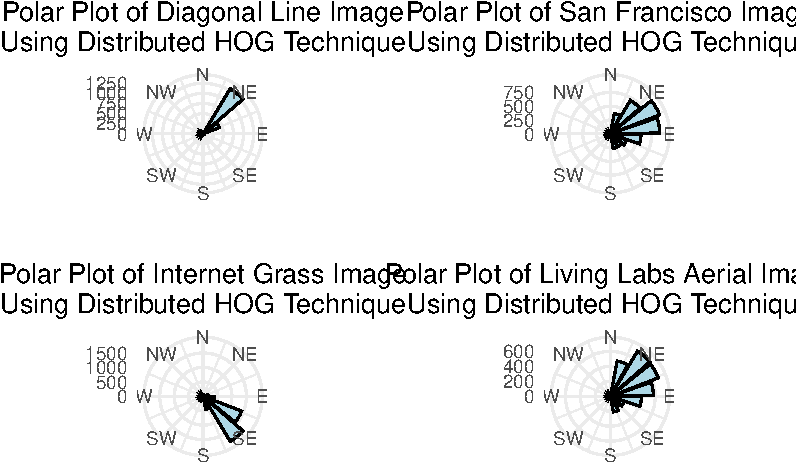
\includegraphics{results_files/figure-pdf/unnamed-chunk-23-1.pdf}

}

\end{figure}

\begin{Shaded}
\begin{Highlighting}[]
\NormalTok{number\_of\_bins }\OperatorTok{=} \DecValTok{9}
\NormalTok{step\_size }\OperatorTok{=} \DecValTok{180} \OperatorTok{/}\NormalTok{ number\_of\_bins}
\end{Highlighting}
\end{Shaded}

\begin{Shaded}
\begin{Highlighting}[]
\CommentTok{\#Function to calculate the value of centre of jth bin}
\KeywordTok{def}\NormalTok{ calculate\_j(angle):}
\NormalTok{  temp }\OperatorTok{=}\NormalTok{ (angle }\OperatorTok{/}\NormalTok{ step\_size) }\OperatorTok{{-}} \FloatTok{0.5}
\NormalTok{  j }\OperatorTok{=}\NormalTok{ math.floor(temp)}
  \ControlFlowTok{return}\NormalTok{ j}
\end{Highlighting}
\end{Shaded}

\begin{Shaded}
\begin{Highlighting}[]
\CommentTok{\# Function to calculate the value of jth bin}
\KeywordTok{def}\NormalTok{ calculate\_Cj(j):}
\NormalTok{  Cj }\OperatorTok{=}\NormalTok{ step\_size }\OperatorTok{*}\NormalTok{ (j }\OperatorTok{+} \FloatTok{0.5}\NormalTok{)}
  \ControlFlowTok{return} \BuiltInTok{round}\NormalTok{(Cj, }\DecValTok{9}\NormalTok{)}
\end{Highlighting}
\end{Shaded}

\begin{Shaded}
\begin{Highlighting}[]
\CommentTok{\# }
\KeywordTok{def}\NormalTok{ calculate\_value\_j(magnitude, angle, j):}
\NormalTok{  Cj }\OperatorTok{=}\NormalTok{ calculate\_Cj(j}\OperatorTok{+}\DecValTok{1}\NormalTok{)}
\NormalTok{  Vj }\OperatorTok{=}\NormalTok{ magnitude }\OperatorTok{*}\NormalTok{ ((Cj }\OperatorTok{{-}}\NormalTok{ angle) }\OperatorTok{/}\NormalTok{ step\_size)}
  \ControlFlowTok{return} \BuiltInTok{round}\NormalTok{(Vj, }\DecValTok{9}\NormalTok{)}
\end{Highlighting}
\end{Shaded}

\begin{Shaded}
\begin{Highlighting}[]
\NormalTok{histogram\_points\_nine }\OperatorTok{=}\NormalTok{ []}
\NormalTok{high\_val }\OperatorTok{=} \DecValTok{10}
\CommentTok{\# for i in range(0, height, high\_val):}
\CommentTok{\#   temp = []}
\CommentTok{\#   for j in range(0, width, high\_val):}
\CommentTok{\#     magnitude\_values = [[mag[i][x] for x in range(j, j+high\_val)] for i in range(i,i+high\_val)]}
\CommentTok{\#     angle\_values = [[theta[i][x] for x in range(j, j+high\_val)] for i in range(i, i+high\_val)]}
\CommentTok{\#     for k in range(len(magnitude\_values)):}
\CommentTok{\#       for l in range(len(magnitude\_values[0])):}
\CommentTok{\#         bins = [0.0 for \_ in range(number\_of\_bins)]}
\CommentTok{\#         value\_j = calculate\_j(angle\_values[k][l])}
\CommentTok{\#         Vj = calculate\_value\_j(magnitude\_values[k][l], angle\_values[k][l], value\_j)}
\CommentTok{\#         Vj\_1 = magnitude\_values[k][l] {-} Vj}
\CommentTok{\#         bins[value\_j]+=Vj}
\CommentTok{\#         bins[value\_j+1]+=Vj\_1}
\CommentTok{\#         bins = [round(x, 9) for x in bins]}
\CommentTok{\#     temp.append(bins)}
\CommentTok{\#   histogram\_points\_nine.append(temp)}
\CommentTok{\# }
\CommentTok{\# print(len(histogram\_points\_nine))}
\CommentTok{\# print(len(histogram\_points\_nine[0]))}
\CommentTok{\# print(len(histogram\_points\_nine[0][0]))}
\end{Highlighting}
\end{Shaded}

\begin{Shaded}
\begin{Highlighting}[]
\NormalTok{epsilon }\OperatorTok{=} \FloatTok{1e{-}05}

\CommentTok{\# feature\_vectors = []}
\CommentTok{\# for i in range(0, len(histogram\_points\_nine) {-} 1, 1):}
\CommentTok{\#   temp = []}
\CommentTok{\#   for j in range(0, len(histogram\_points\_nine[0]) {-} 1, 1):}
\CommentTok{\#     values = [[histogram\_points\_nine[i][x] for x in range(j, j+2)] for i in range(i, i+2)]}
\CommentTok{\#     final\_vector = []}
\CommentTok{\#     for k in values:}
\CommentTok{\#       for l in k:}
\CommentTok{\#         for m in l:}
\CommentTok{\#           final\_vector.append(m)}
\CommentTok{\#     k = round(math.sqrt(sum([pow(x, 2) for x in final\_vector])), 9)}
\CommentTok{\#     final\_vector = [round(x/(k + epsilon), 9) for x in final\_vector]}
\CommentTok{\#     temp.append(final\_vector)}
\CommentTok{\#   feature\_vectors.append(temp)}
\CommentTok{\#   }
\CommentTok{\# print(len(feature\_vectors))}
\CommentTok{\# print(len(feature\_vectors[0]))}
\CommentTok{\# print(len(feature\_vectors[0][0]))}
\end{Highlighting}
\end{Shaded}

\hypertarget{generate-hog-image}{%
\section{Generate HOG Image}\label{generate-hog-image}}

\begin{Shaded}
\begin{Highlighting}[]
\NormalTok{img }\OperatorTok{=}\NormalTok{ imread(}\StringTok{"images/living\_lab\_aerial/aerial\_grass\_living\_lab\_rotated.jpg"}\NormalTok{)}
\NormalTok{img }\OperatorTok{=}\NormalTok{ color.rgb2gray(io.imread(}\StringTok{"images/grass\_image2.jpg"}\NormalTok{))}

\NormalTok{aspect\_ratio }\OperatorTok{=}\NormalTok{ img.shape[}\DecValTok{0}\NormalTok{]}\OperatorTok{/}\NormalTok{img.shape[}\DecValTok{1}\NormalTok{]}

\NormalTok{height }\OperatorTok{=} \DecValTok{200}
\NormalTok{width }\OperatorTok{=} \BuiltInTok{int}\NormalTok{(height}\OperatorTok{/}\NormalTok{aspect\_ratio)}

\CommentTok{\# height = 128}
\CommentTok{\# width = 192}

\CommentTok{\# make sure the resized is in sample ball park as the original aspect ratio, }
\CommentTok{\# that way the angles don\textquotesingle{}t get squished}
\NormalTok{resized\_ratio }\OperatorTok{=}\NormalTok{ height}\OperatorTok{/}\NormalTok{width}


\NormalTok{resized\_img }\OperatorTok{=}\NormalTok{ resize(img, (height, width))}

\NormalTok{plt.axis(}\StringTok{"off"}\NormalTok{)}
\end{Highlighting}
\end{Shaded}

\begin{verbatim}
(0.0, 1.0, 0.0, 1.0)
\end{verbatim}

\begin{Shaded}
\begin{Highlighting}[]
\NormalTok{plt.imshow(resized\_img)}
\BuiltInTok{print}\NormalTok{(resized\_img.shape)}
\end{Highlighting}
\end{Shaded}

\begin{verbatim}
(200, 301)
\end{verbatim}

\begin{Shaded}
\begin{Highlighting}[]
\NormalTok{fd, hog\_image }\OperatorTok{=}\NormalTok{ hog(resized\_img, orientations}\OperatorTok{=}\DecValTok{9}\NormalTok{, pixels\_per\_cell}\OperatorTok{=}\NormalTok{(}\DecValTok{8}\NormalTok{, }\DecValTok{8}\NormalTok{),}
\NormalTok{                    cells\_per\_block}\OperatorTok{=}\NormalTok{(}\DecValTok{2}\NormalTok{, }\DecValTok{2}\NormalTok{), visualize}\OperatorTok{=}\VariableTok{True}\CommentTok{\#, channel\_axis = 2 }
                    \CommentTok{\#multichannel=True}
\NormalTok{                    )}
\NormalTok{plt.axis(}\StringTok{"off"}\NormalTok{)}
\end{Highlighting}
\end{Shaded}

\begin{verbatim}
(-0.5, 300.5, 199.5, -0.5)
\end{verbatim}

\begin{Shaded}
\begin{Highlighting}[]
\NormalTok{plt.imshow(hog\_image, cmap}\OperatorTok{=}\StringTok{"gray"}\NormalTok{)}
\NormalTok{plt.show()}
\end{Highlighting}
\end{Shaded}

\begin{figure}[H]

{\centering 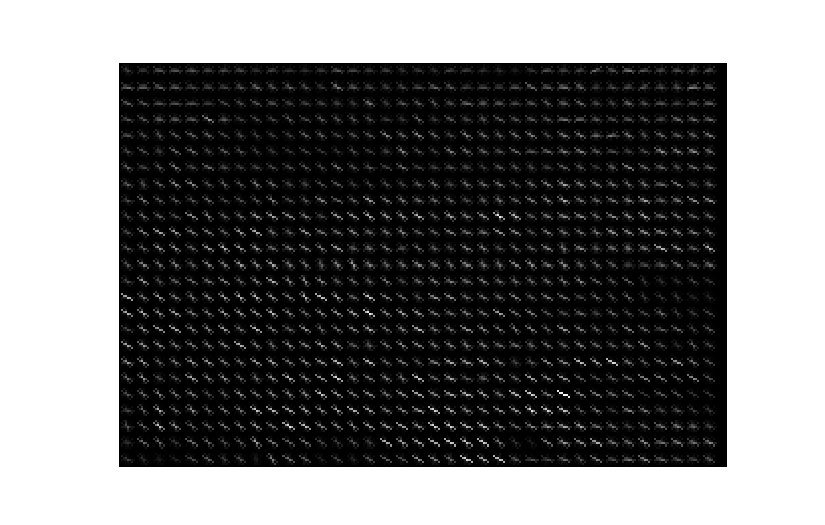
\includegraphics{results_files/figure-pdf/unnamed-chunk-30-1.pdf}

}

\end{figure}

\begin{Shaded}
\begin{Highlighting}[]
\NormalTok{plt.savefig(}\StringTok{\textquotesingle{}images/plots/grass2\_image\_hog.jpg\textquotesingle{}}\NormalTok{)}
\end{Highlighting}
\end{Shaded}

\begin{figure}[H]

{\centering 
\includegraphics{results_files/figure-pdf/unnamed-chunk-30-2.pdf}

}

\end{figure}

\begin{Shaded}
\begin{Highlighting}[]
\CommentTok{\# grass2\_polar\_plot \textless{}{-}}
\CommentTok{\# ggplot(diagonal\_hog\_df, \#\%\textgreater{}\% filter(mag \textgreater{}= 0.1), }
\CommentTok{\#        aes(x = radian)) +}
\CommentTok{\#   geom\_histogram(colour = "black", fill = "lightblue", }
\CommentTok{\#                  breaks = seq(0, 2*pi, length.out = 17.5),}
\CommentTok{\#                  bins = 9) +}
\CommentTok{\#   coord\_polar(}
\CommentTok{\#     theta = "x", start = 0, direction = 1) +}
\CommentTok{\#   scale\_x\_continuous(}
\CommentTok{\#     breaks = c(0, pi/4, pi/2, 3*pi/4, pi, 5*pi/4, 3*pi/2, 7*pi/4), }
\CommentTok{\#     labels = c("N", "NE", "E", "SE", "S", "SW", "W", "NW")}
\CommentTok{\#   )+}
\CommentTok{\#   labs(title = "Polar Plot of Internet Grass Image") +}
\CommentTok{\#     theme\_minimal() +}
\CommentTok{\#   labs(x = "") +}
\CommentTok{\#   theme(axis.title.y = element\_blank(),}
\CommentTok{\#         plot.title = element\_text(hjust = 0.5))}
\CommentTok{\# }
\CommentTok{\# grass2\_polar\_plot}

\CommentTok{\#ggsave("\_polar\_plot.jpg", polar\_plot, width = 6, height = 4, dpi = 300)}

\CommentTok{\#all\_plots \textless{}{-} ggpubr::ggarrange(diaganol\_polar\_plot, sf\_polar\_plot, grass2\_polar\_plot, aerial\_ll\_polar\_plot)}

\CommentTok{\#ggsave("images/plots/results\_all\_plots.jpg", all\_plots, width = 7, height = 7)}
\end{Highlighting}
\end{Shaded}

\hypertarget{hog-image-of-internet-grass}{%
\section{HOG Image of Internet
Grass}\label{hog-image-of-internet-grass}}

\begin{Shaded}
\begin{Highlighting}[]
\ImportTok{from}\NormalTok{ skimage }\ImportTok{import}\NormalTok{ color, io, exposure}
\ImportTok{from}\NormalTok{ skimage.transform }\ImportTok{import}\NormalTok{ resize}
\ImportTok{import}\NormalTok{ matplotlib.pyplot }\ImportTok{as}\NormalTok{ plt}
\ImportTok{from}\NormalTok{ skimage.feature }\ImportTok{import}\NormalTok{ hog}

\CommentTok{\# Load the image and preprocess it}
\NormalTok{img }\OperatorTok{=}\NormalTok{ color.rgb2gray(io.imread(}\StringTok{"images/grass\_image2.jpg"}\NormalTok{))}
\CommentTok{\# img = color.rgb2gray(io.imread("diagnol\_lines\_flipped.jpg"))}

\NormalTok{aspect\_ratio }\OperatorTok{=}\NormalTok{ img.shape[}\DecValTok{0}\NormalTok{] }\OperatorTok{/}\NormalTok{ img.shape[}\DecValTok{1}\NormalTok{]}
\NormalTok{height }\OperatorTok{=} \DecValTok{200}
\NormalTok{width }\OperatorTok{=} \BuiltInTok{int}\NormalTok{(height }\OperatorTok{/}\NormalTok{ aspect\_ratio)}
\NormalTok{resized\_img }\OperatorTok{=}\NormalTok{ resize(img, (height, width))}

\NormalTok{plt.figure(figsize}\OperatorTok{=}\NormalTok{(}\DecValTok{8}\NormalTok{, }\DecValTok{20}\NormalTok{))  }\CommentTok{\# Adjusted the figure size to accommodate the additional object}
\NormalTok{plt.imshow(resized\_img, cmap}\OperatorTok{=}\StringTok{"gray"}\NormalTok{)}
\NormalTok{plt.axis(}\StringTok{"off"}\NormalTok{)}
\end{Highlighting}
\end{Shaded}

\begin{verbatim}
(-0.5, 300.5, 199.5, -0.5)
\end{verbatim}

\begin{Shaded}
\begin{Highlighting}[]
\NormalTok{plt.show()}
\end{Highlighting}
\end{Shaded}

\begin{figure}[H]

{\centering 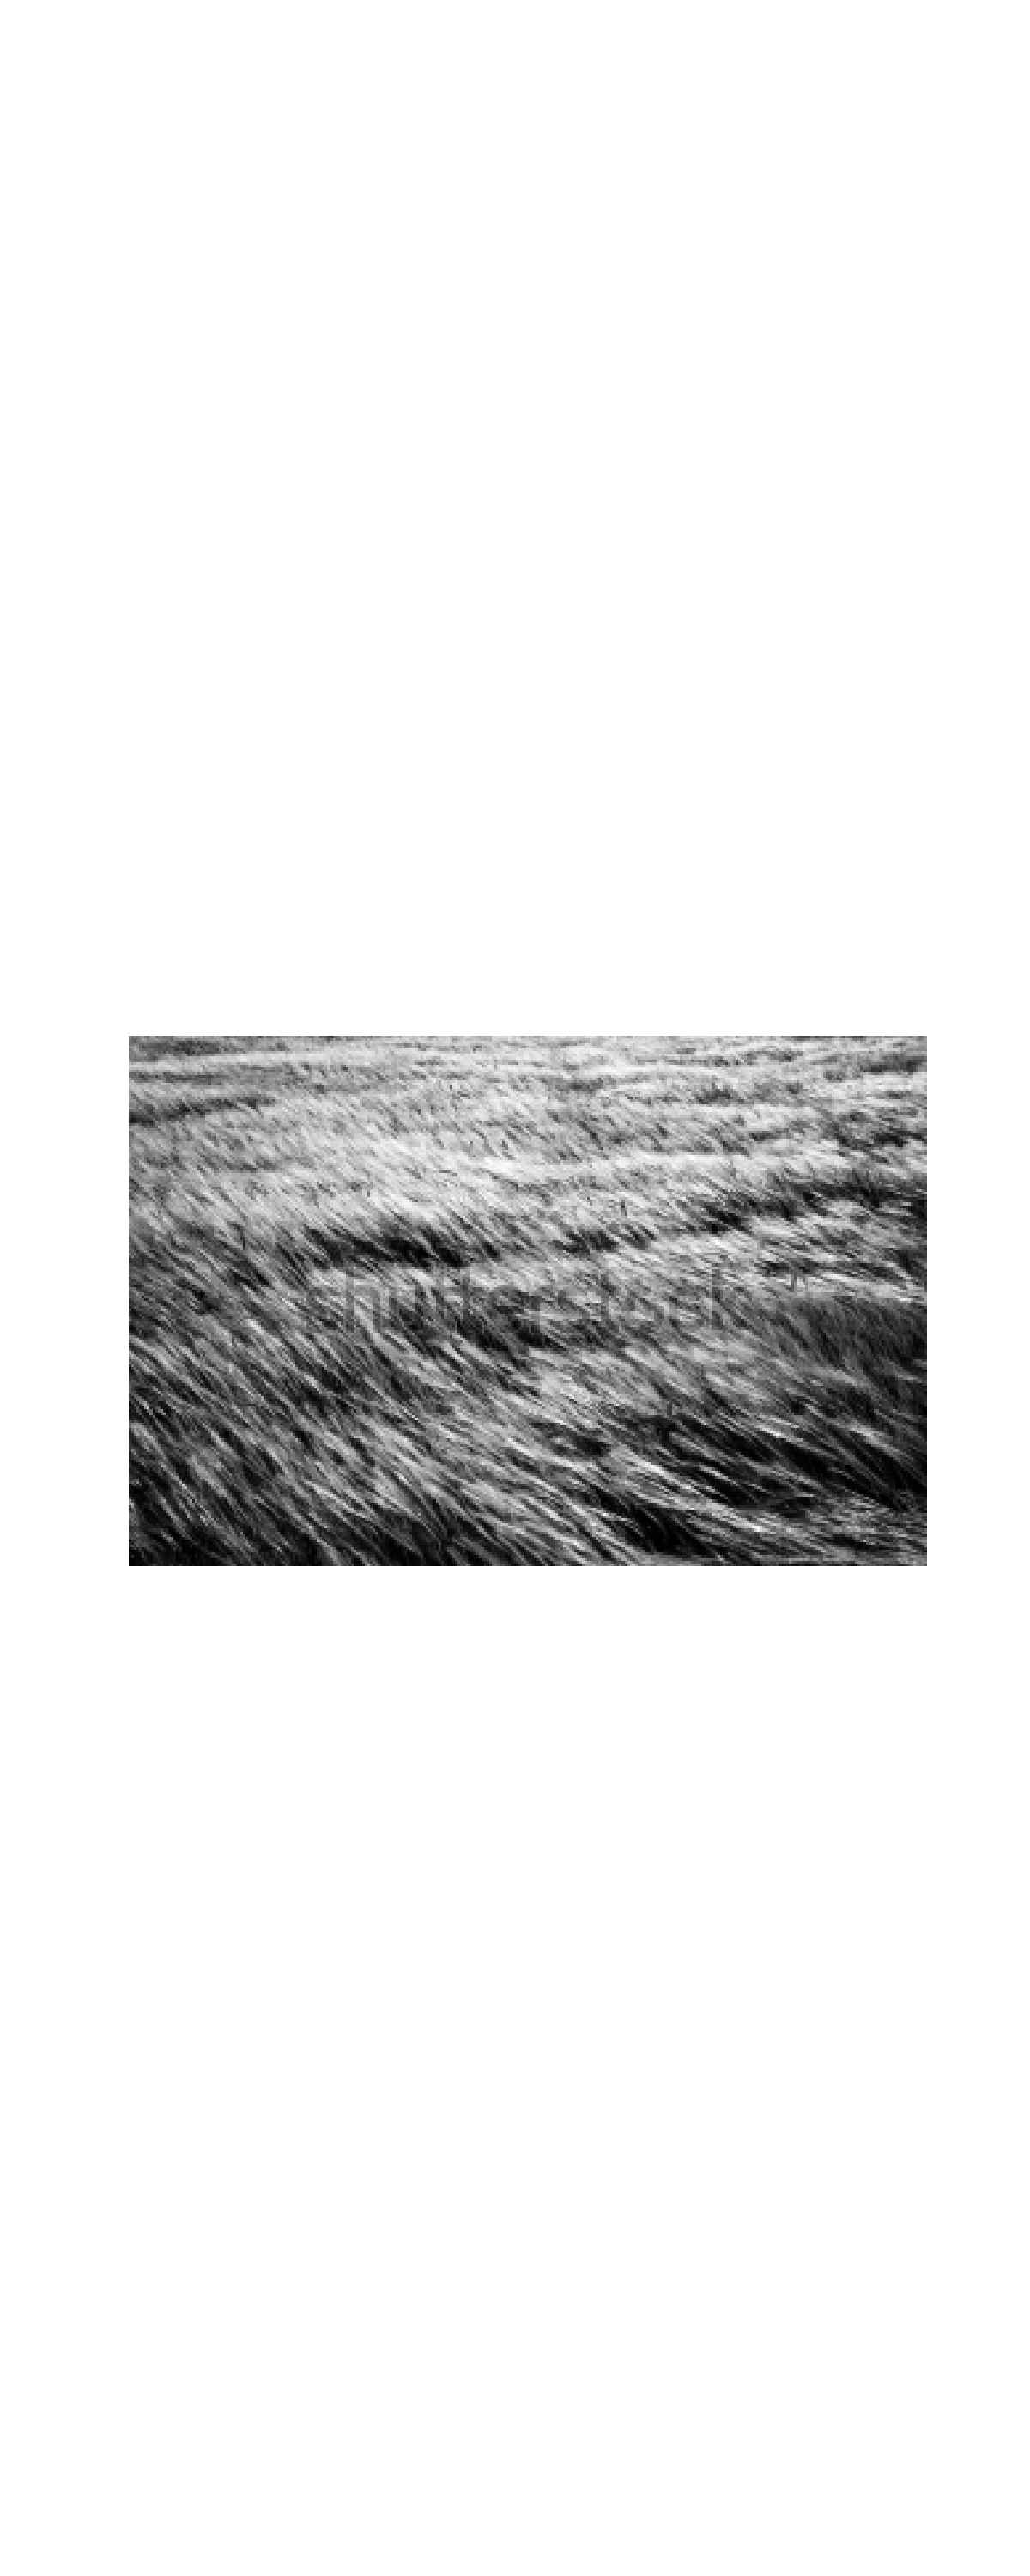
\includegraphics{results_files/figure-pdf/unnamed-chunk-32-1.pdf}

}

\end{figure}

\begin{Shaded}
\begin{Highlighting}[]
\CommentTok{\# Compute HOG features}
\NormalTok{hog\_features, hog\_image }\OperatorTok{=}\NormalTok{ hog(resized\_img, orientations}\OperatorTok{=}\DecValTok{9}\NormalTok{, pixels\_per\_cell}\OperatorTok{=}\NormalTok{(}\DecValTok{8}\NormalTok{,}\DecValTok{8}\NormalTok{),}
\NormalTok{                              cells\_per\_block}\OperatorTok{=}\NormalTok{(}\DecValTok{10}\NormalTok{, }\DecValTok{10}\NormalTok{), visualize}\OperatorTok{=}\VariableTok{True}\NormalTok{)}

\CommentTok{\# Plot the images}
\NormalTok{fig, (ax1, ax2, ax3) }\OperatorTok{=}\NormalTok{ plt.subplots(}\DecValTok{3}\NormalTok{, }\DecValTok{1}\NormalTok{, figsize}\OperatorTok{=}\NormalTok{(}\DecValTok{8}\NormalTok{, }\DecValTok{20}\NormalTok{), sharex}\OperatorTok{=}\VariableTok{True}\NormalTok{, sharey}\OperatorTok{=}\VariableTok{True}\NormalTok{)  }\CommentTok{\# Changed 1, 2 to 3, 1}

\CommentTok{\# Plot the rescaled black and white image}
\NormalTok{ax1.imshow(resized\_img, cmap}\OperatorTok{=}\NormalTok{plt.cm.gray)}
\NormalTok{ax1.set\_title(}\StringTok{\textquotesingle{}Rescaled Black and White Image\textquotesingle{}}\NormalTok{)}

\CommentTok{\# Plot the mag object}
\NormalTok{ax2.imshow(mag, cmap}\OperatorTok{=}\NormalTok{plt.cm.gray)  }\CommentTok{\# Assuming mag is the object you want to insert}
\CommentTok{\#ax2.axis("off")}
\NormalTok{ax2.set\_title(}\StringTok{\textquotesingle{}Pixel Magnitudes\textquotesingle{}}\NormalTok{)}

\CommentTok{\# rescale HOG for better viewing:}
\NormalTok{hog\_color\_rescaled }\OperatorTok{=}\NormalTok{ exposure.rescale\_intensity(hog\_image, in\_range}\OperatorTok{=}\NormalTok{(}\DecValTok{0}\NormalTok{, }\DecValTok{10}\NormalTok{))}

\CommentTok{\# Plot the histogram of oriented gradients}
\NormalTok{ax3.imshow(hog\_color\_rescaled, cmap}\OperatorTok{=}\NormalTok{plt.cm.gray)}
\NormalTok{ax3.set\_title(}\StringTok{\textquotesingle{}Histogram of Oriented Gradients (HOG)\textquotesingle{}}\NormalTok{)}

\NormalTok{plt.savefig(}\StringTok{"images/plots/rescaled\_grass2\_image\_hog.png"}\NormalTok{, dpi}\OperatorTok{=}\DecValTok{300}\NormalTok{)}

\NormalTok{plt.show()}
\end{Highlighting}
\end{Shaded}

\begin{figure}[H]

{\centering 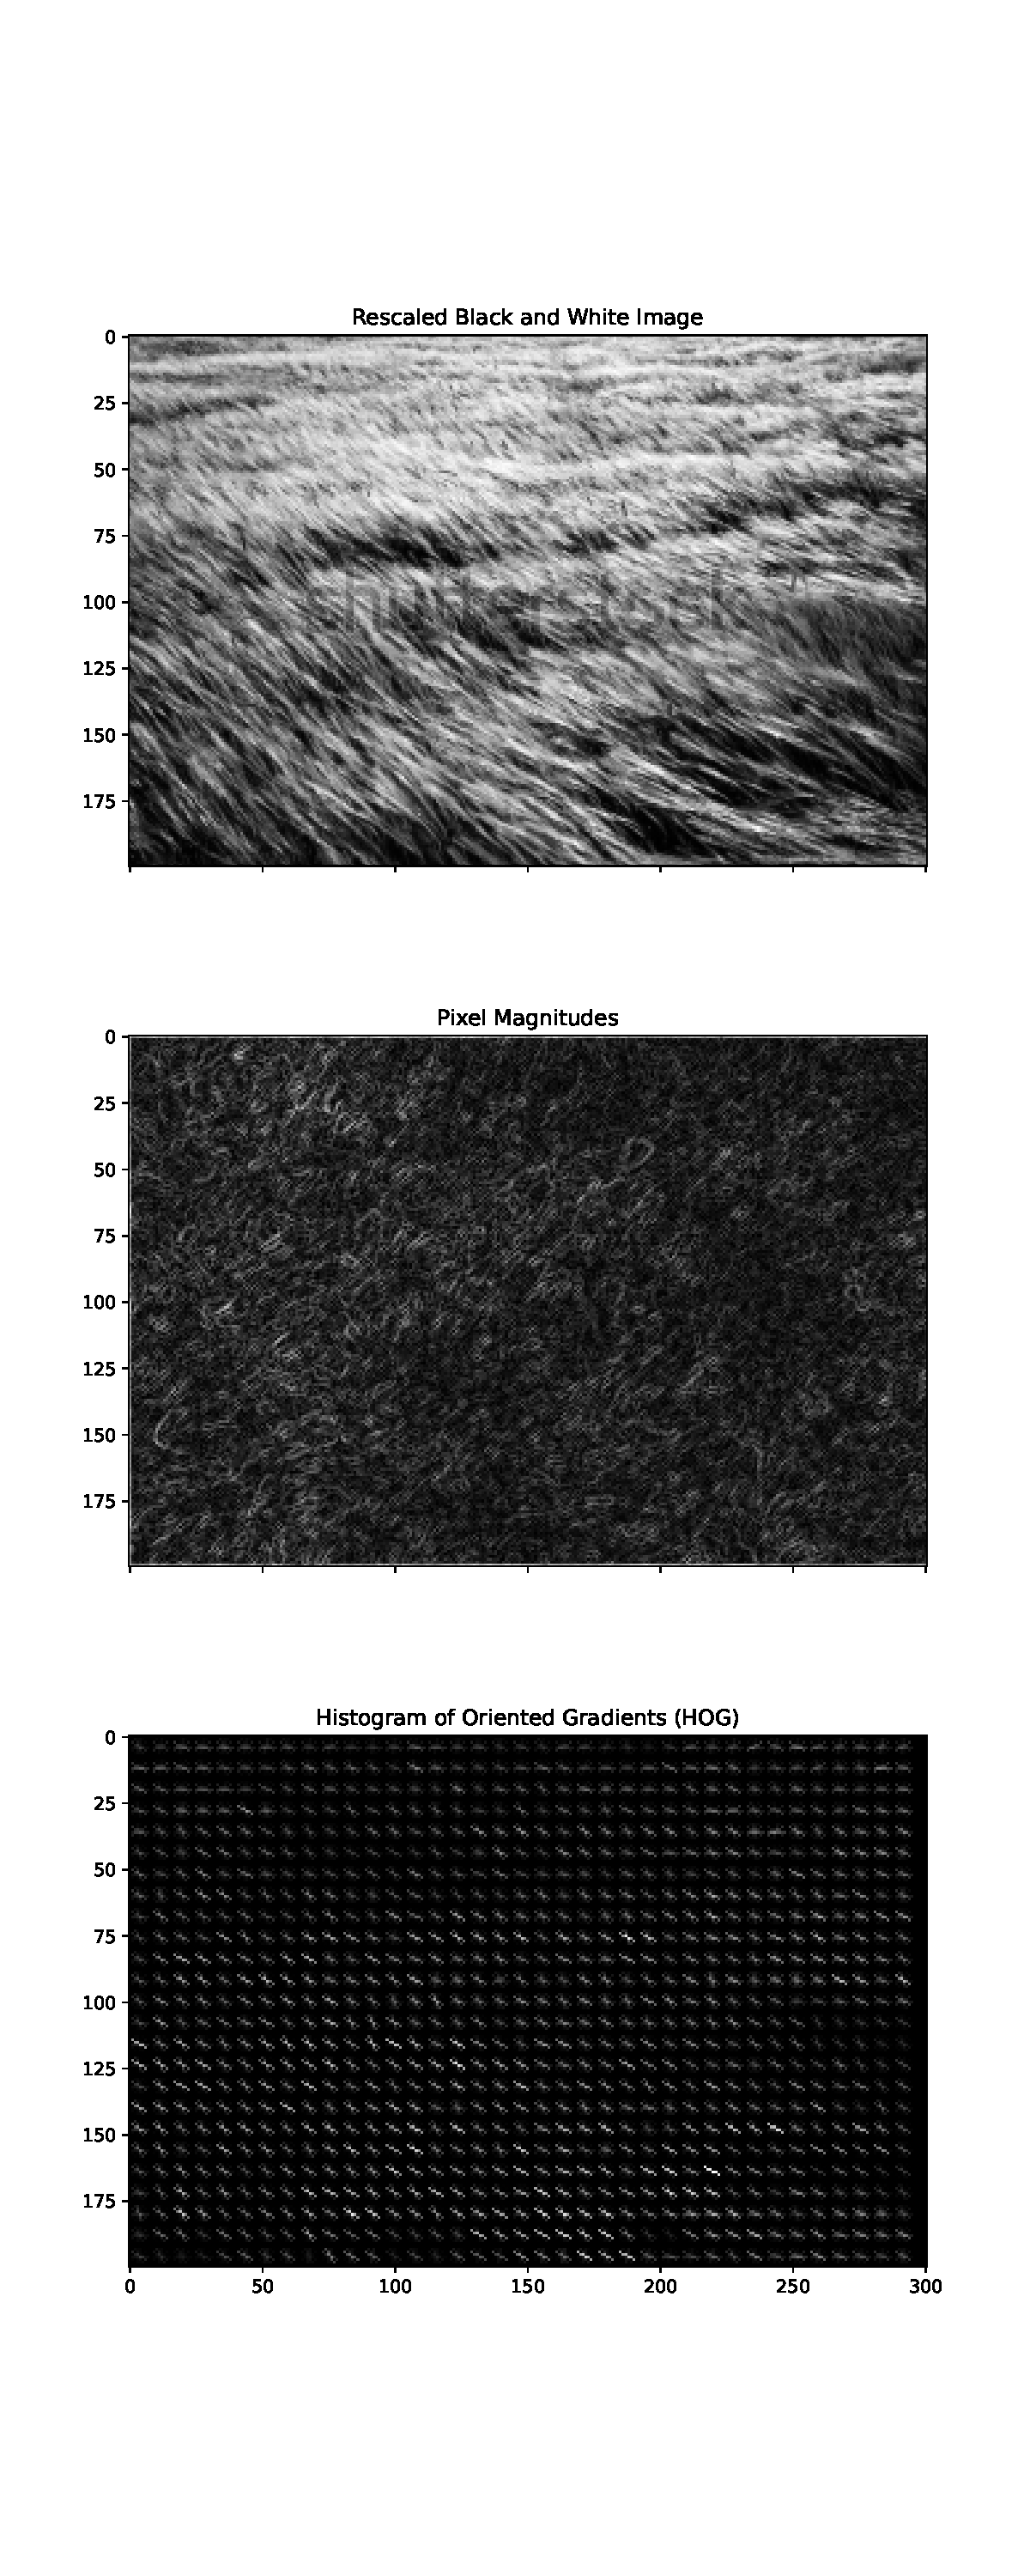
\includegraphics{results_files/figure-pdf/unnamed-chunk-32-2.pdf}

}

\end{figure}

\begin{Shaded}
\begin{Highlighting}[]
\ImportTok{from}\NormalTok{ skimage }\ImportTok{import}\NormalTok{ color, io, exposure}
\ImportTok{from}\NormalTok{ skimage.transform }\ImportTok{import}\NormalTok{ resize}
\ImportTok{import}\NormalTok{ matplotlib.pyplot }\ImportTok{as}\NormalTok{ plt}
\ImportTok{from}\NormalTok{ skimage.feature }\ImportTok{import}\NormalTok{ hog}

\CommentTok{\# Load the image and preprocess it}
\NormalTok{img }\OperatorTok{=}\NormalTok{ io.imread(}\StringTok{"images/grass\_image2.jpg"}\NormalTok{)}
\CommentTok{\# img = color.rgb2gray(io.imread("diagnol\_lines\_flipped.jpg"))}

\NormalTok{aspect\_ratio }\OperatorTok{=}\NormalTok{ img.shape[}\DecValTok{0}\NormalTok{] }\OperatorTok{/}\NormalTok{ img.shape[}\DecValTok{1}\NormalTok{]}
\NormalTok{height }\OperatorTok{=} \DecValTok{200}
\NormalTok{width }\OperatorTok{=} \BuiltInTok{int}\NormalTok{(height }\OperatorTok{/}\NormalTok{ aspect\_ratio)}
\NormalTok{resized\_img }\OperatorTok{=}\NormalTok{ resize(img, (height, width))}

\NormalTok{bw\_resized\_image }\OperatorTok{=}\NormalTok{ color.rgb2gray(resized\_img)}

\NormalTok{plt.figure(figsize}\OperatorTok{=}\NormalTok{(}\DecValTok{15}\NormalTok{, }\DecValTok{5}\NormalTok{))  }\CommentTok{\# Adjusted the figure size to accommodate the additional object}
\NormalTok{plt.imshow(resized\_img, cmap}\OperatorTok{=}\StringTok{"gray"}\NormalTok{)}
\NormalTok{plt.axis(}\StringTok{"off"}\NormalTok{)}
\end{Highlighting}
\end{Shaded}

\begin{verbatim}
(-0.5, 300.5, 199.5, -0.5)
\end{verbatim}

\begin{Shaded}
\begin{Highlighting}[]
\NormalTok{plt.show()}
\end{Highlighting}
\end{Shaded}

\begin{figure}[H]

{\centering 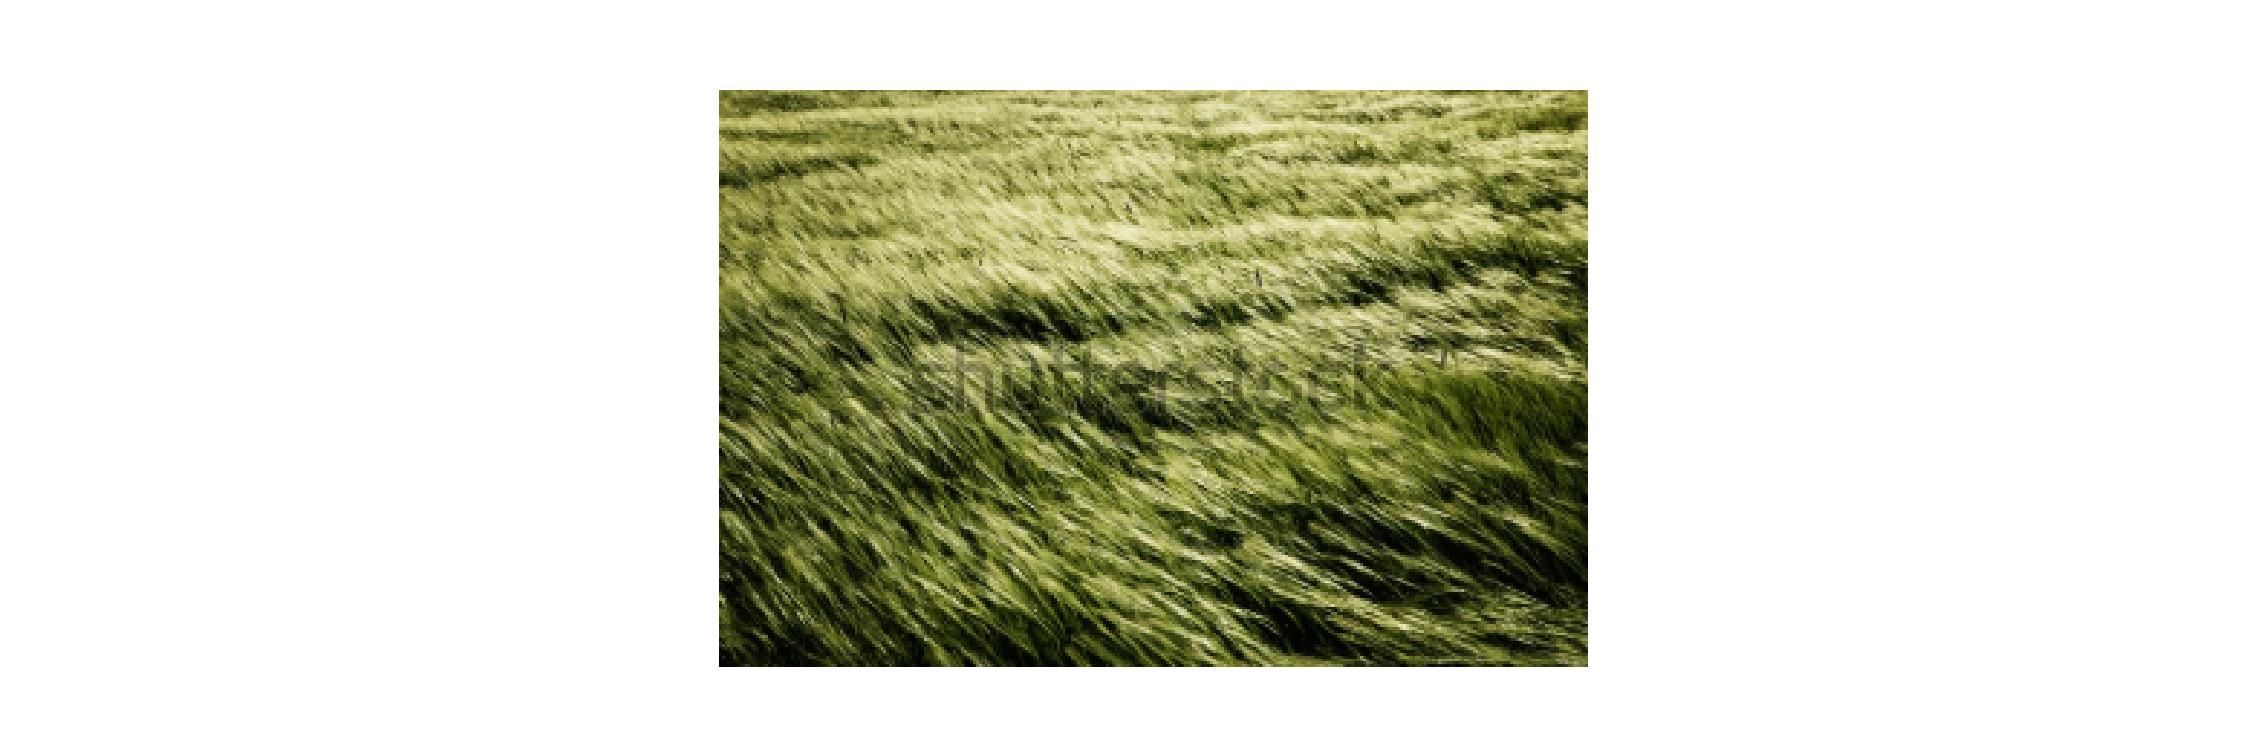
\includegraphics{results_files/figure-pdf/unnamed-chunk-33-5.pdf}

}

\end{figure}

\begin{Shaded}
\begin{Highlighting}[]
\CommentTok{\# Compute HOG features}
\NormalTok{hog\_features, hog\_image }\OperatorTok{=}\NormalTok{ hog(bw\_resized\_image, orientations}\OperatorTok{=}\DecValTok{9}\NormalTok{, pixels\_per\_cell}\OperatorTok{=}\NormalTok{(}\DecValTok{8}\NormalTok{,}\DecValTok{8}\NormalTok{),}
\NormalTok{                              cells\_per\_block}\OperatorTok{=}\NormalTok{(}\DecValTok{10}\NormalTok{, }\DecValTok{10}\NormalTok{), visualize}\OperatorTok{=}\VariableTok{True}\NormalTok{)}

\CommentTok{\# Plot the images}
\NormalTok{fig, (ax1, ax2, ax3) }\OperatorTok{=}\NormalTok{ plt.subplots(}\DecValTok{1}\NormalTok{, }\DecValTok{3}\NormalTok{, figsize}\OperatorTok{=}\NormalTok{(}\DecValTok{25}\NormalTok{, }\DecValTok{5}\NormalTok{), sharex}\OperatorTok{=}\VariableTok{True}\NormalTok{, sharey}\OperatorTok{=}\VariableTok{True}\NormalTok{)  }\CommentTok{\# Changed 3, 1 to 1, 5}

\CommentTok{\# Plot the rescaled input image}
\NormalTok{ax1.imshow(resized\_img, cmap}\OperatorTok{=}\NormalTok{plt.cm.gray)}
\NormalTok{ax1.set\_title(}\StringTok{\textquotesingle{}Rescaled Input Image\textquotesingle{}}\NormalTok{)}

\CommentTok{\# Plot the pixel magnitudes}
\NormalTok{ax2.imshow(mag, cmap}\OperatorTok{=}\NormalTok{plt.cm.gray)  }\CommentTok{\# Assuming mag is the object you want to insert}
\NormalTok{ax2.set\_title(}\StringTok{\textquotesingle{}Pixel Magnitudes\textquotesingle{}}\NormalTok{)}

\CommentTok{\# Plot the histogram of oriented gradients}
\NormalTok{hog\_color\_rescaled }\OperatorTok{=}\NormalTok{ exposure.rescale\_intensity(hog\_image, in\_range}\OperatorTok{=}\NormalTok{(}\DecValTok{0}\NormalTok{, }\DecValTok{10}\NormalTok{))}
\NormalTok{ax3.imshow(hog\_color\_rescaled, cmap}\OperatorTok{=}\NormalTok{plt.cm.gray)}
\NormalTok{ax3.set\_title(}\StringTok{\textquotesingle{}Histogram of Oriented Gradients (HOG) Image\textquotesingle{}}\NormalTok{)}

\CommentTok{\# Plot the histogram of oriented gradients}
\CommentTok{\# angle\_hist = io.imread("images/grass2\_angles\_histogram.jpg")}
\CommentTok{\# resized\_hist = resize(angle\_hist, (height, width))}
\CommentTok{\# ax4.imshow(resized\_hist, cmap=plt.cm.gray)}
\CommentTok{\# ax4.set\_title(\textquotesingle{}Angle Histogram\textquotesingle{})}
\CommentTok{\# }
\CommentTok{\# \# Plot the polar plot}
\CommentTok{\# polar\_plot = io.imread("images/grass2\_polar\_plot.jpg")}
\CommentTok{\# resized\_polar = resize(polar\_plot, (height, width))}
\CommentTok{\# ax5.imshow(resized\_polar, cmap=plt.cm.gray)}
\CommentTok{\# ax5.set\_title(\textquotesingle{}Polar Plot\textquotesingle{})}

\NormalTok{plt.savefig(}\StringTok{"images/plots/rescaled\_grass2\_image\_hog.png"}\NormalTok{, dpi}\OperatorTok{=}\DecValTok{300}\NormalTok{)}

\NormalTok{plt.show()}
\end{Highlighting}
\end{Shaded}

\begin{figure}[H]

{\centering 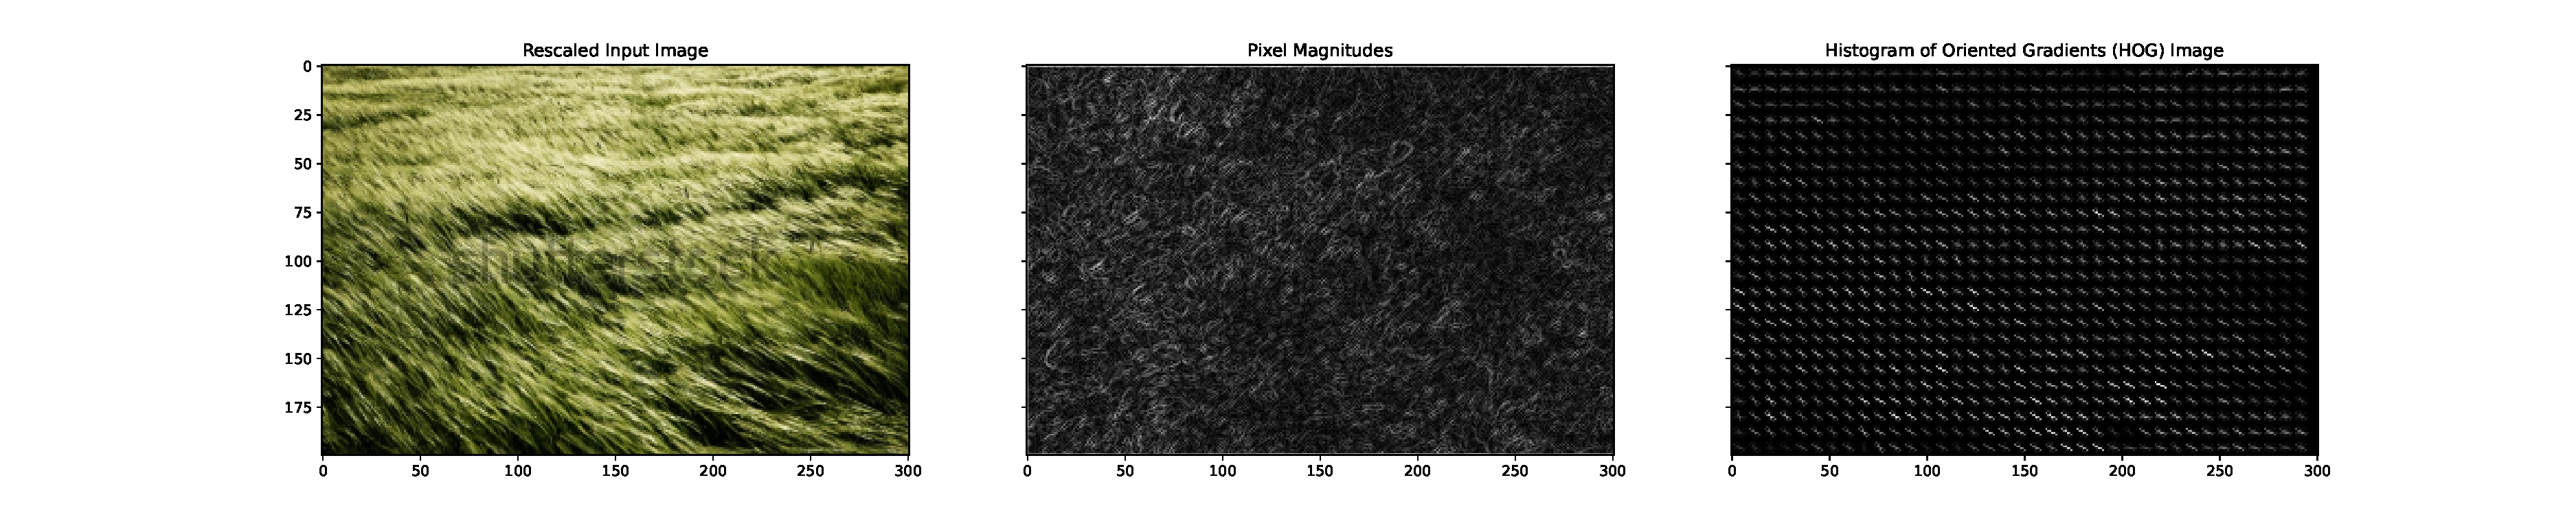
\includegraphics{results_files/figure-pdf/unnamed-chunk-33-6.pdf}

}

\end{figure}

\hypertarget{titus-flip}{%
\section{Titus Flip}\label{titus-flip}}

\begin{Shaded}
\begin{Highlighting}[]
\NormalTok{image }\OperatorTok{=}\NormalTok{ imread(}\StringTok{\textquotesingle{}images/TitusFlip.jpg\textquotesingle{}}\NormalTok{)}
\NormalTok{imshow(image)}
\BuiltInTok{print}\NormalTok{(image.shape)}
\end{Highlighting}
\end{Shaded}

\begin{verbatim}
(1350, 1080, 3)
\end{verbatim}

\begin{Shaded}
\begin{Highlighting}[]
\NormalTok{resized\_image }\OperatorTok{=}\NormalTok{ resize(image, (}\DecValTok{300}\NormalTok{, }\DecValTok{400}\NormalTok{))}
\CommentTok{\#resized\_image = image}
\NormalTok{imshow(resized\_image)}
\BuiltInTok{print}\NormalTok{(resized\_image.shape)}
\end{Highlighting}
\end{Shaded}

\begin{verbatim}
(300, 400, 3)
\end{verbatim}

\begin{Shaded}
\begin{Highlighting}[]
\NormalTok{fig, hog\_image }\OperatorTok{=}\NormalTok{ hog(resized\_image, orientations}\OperatorTok{=}\DecValTok{9}\NormalTok{, pixels\_per\_cell}\OperatorTok{=}\NormalTok{(}\DecValTok{3}\NormalTok{, }\DecValTok{3}\NormalTok{),}
\NormalTok{                     cells\_per\_block}\OperatorTok{=}\NormalTok{(}\DecValTok{15}\NormalTok{, }\DecValTok{15}\NormalTok{), visualize}\OperatorTok{=}\VariableTok{True}\NormalTok{, channel\_axis}\OperatorTok{=}\DecValTok{2} \CommentTok{\#multichannel=True}
\NormalTok{                     )}
\NormalTok{fig, (ax1, ax2) }\OperatorTok{=}\NormalTok{ plt.subplots(}\DecValTok{1}\NormalTok{, }\DecValTok{2}\NormalTok{, figsize}\OperatorTok{=}\NormalTok{(}\DecValTok{16}\NormalTok{, }\DecValTok{7}\NormalTok{), sharex}\OperatorTok{=}\VariableTok{True}\NormalTok{, sharey}\OperatorTok{=}\VariableTok{True}\NormalTok{)}

\NormalTok{ax1.imshow(resized\_image, cmap}\OperatorTok{=}\NormalTok{plt.cm.gray)}
\NormalTok{ax1.set\_title(}\StringTok{\textquotesingle{}Input image\textquotesingle{}}\NormalTok{)}

\CommentTok{\# Rescale histogram for better display }
\NormalTok{hog\_color\_rescaled }\OperatorTok{=}\NormalTok{ exposure.rescale\_intensity(hog\_image, in\_range}\OperatorTok{=}\NormalTok{(}\DecValTok{0}\NormalTok{, }\DecValTok{10}\NormalTok{))}

\NormalTok{ax2.imshow(hog\_color\_rescaled, cmap}\OperatorTok{=}\NormalTok{plt.cm.gray)}
\NormalTok{ax2.set\_title(}\StringTok{\textquotesingle{}Histogram of Oriented Gradients (HOG)\textquotesingle{}}\NormalTok{)}

\CommentTok{\# store to file}
\NormalTok{plt.savefig(}\StringTok{"images/plots/titus\_flip\_example\_hog.png"}\NormalTok{, dpi}\OperatorTok{=}\DecValTok{300}\NormalTok{)}

\NormalTok{plt.show()}
\end{Highlighting}
\end{Shaded}

\begin{figure}[H]

{\centering 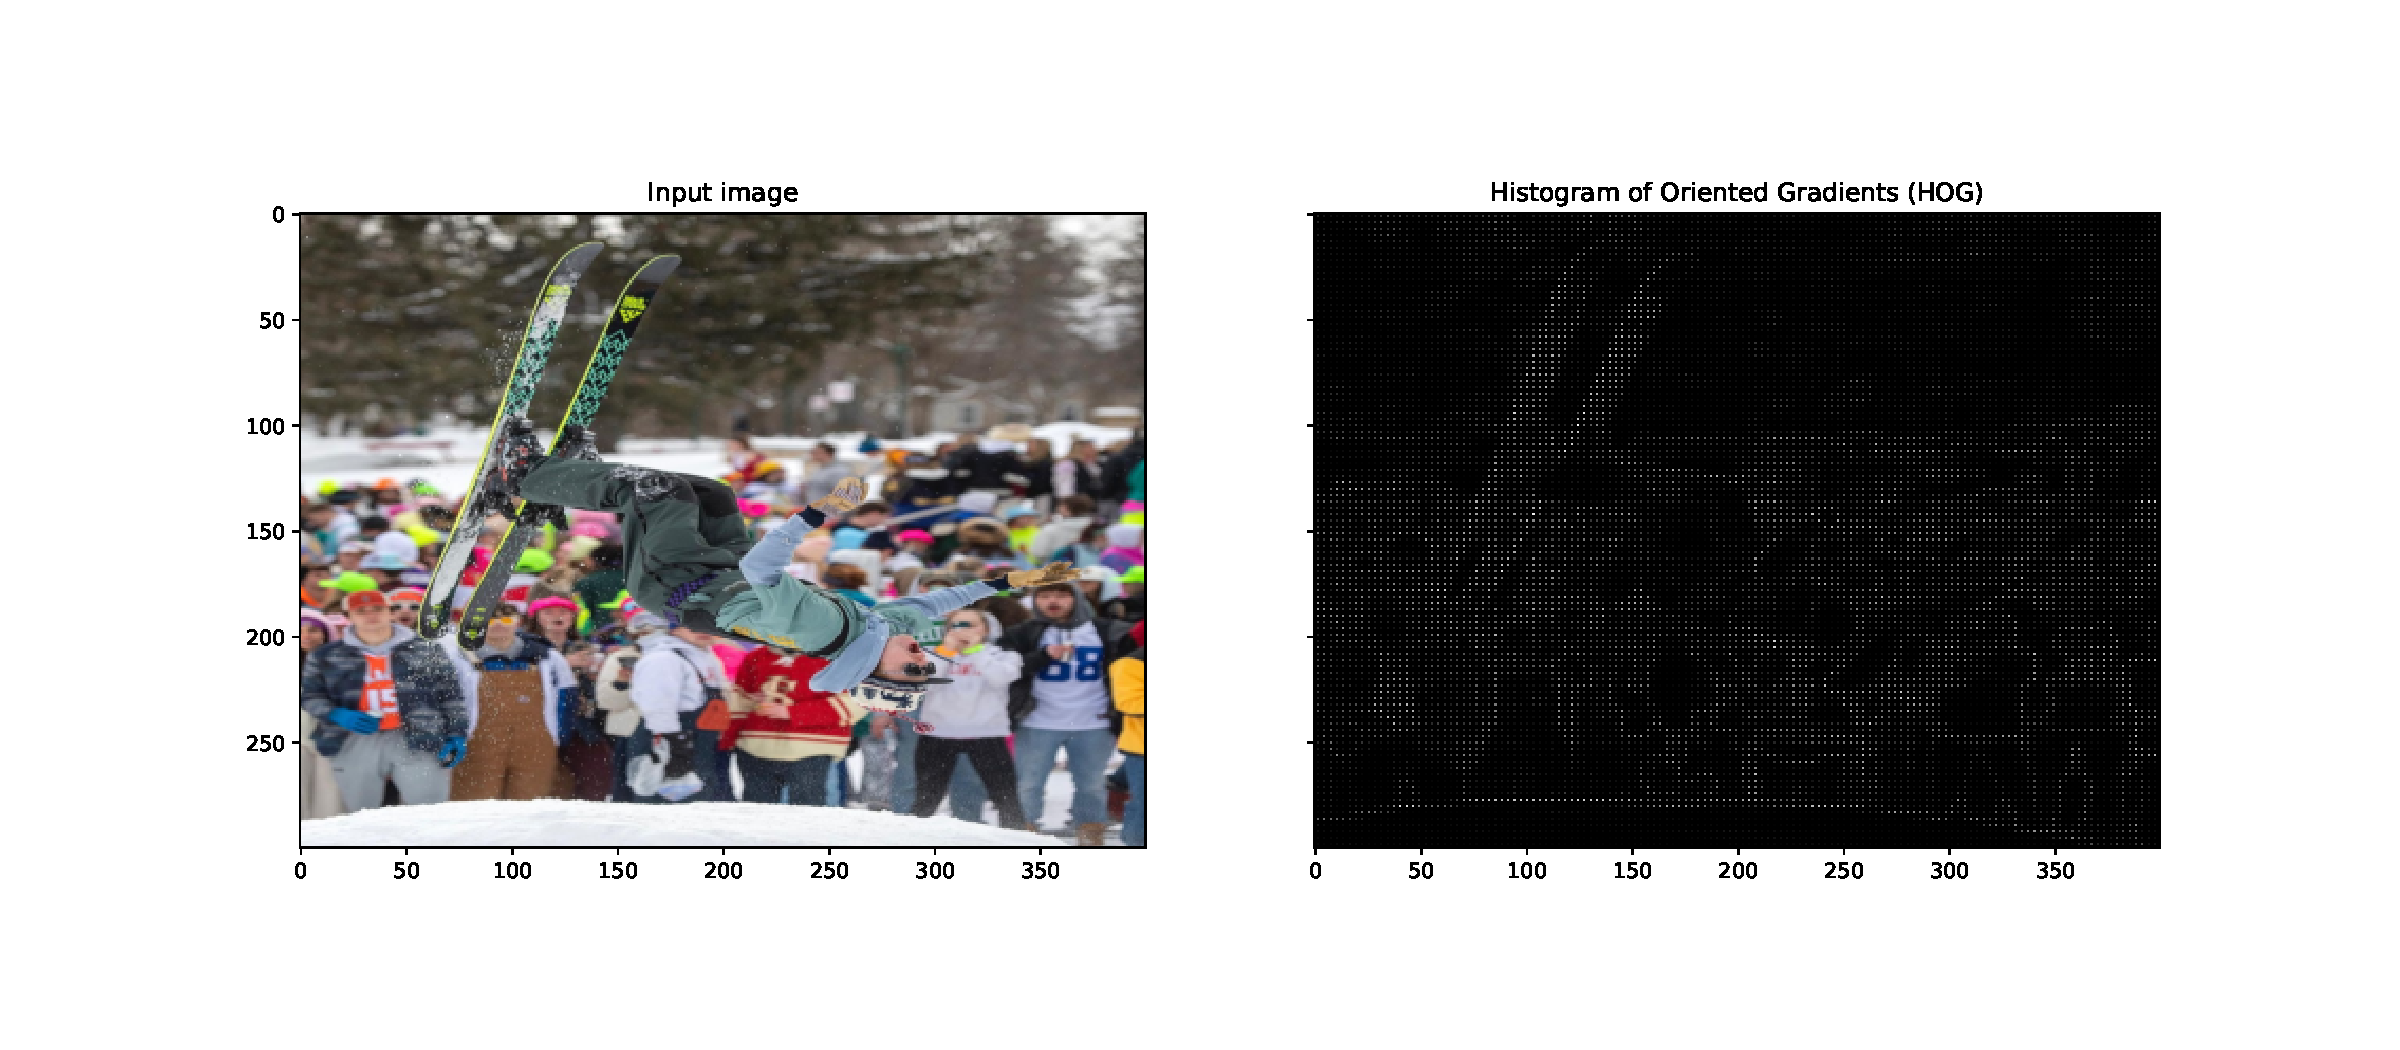
\includegraphics{results_files/figure-pdf/unnamed-chunk-34-9.pdf}

}

\end{figure}

\begin{figure}[H]

{\centering 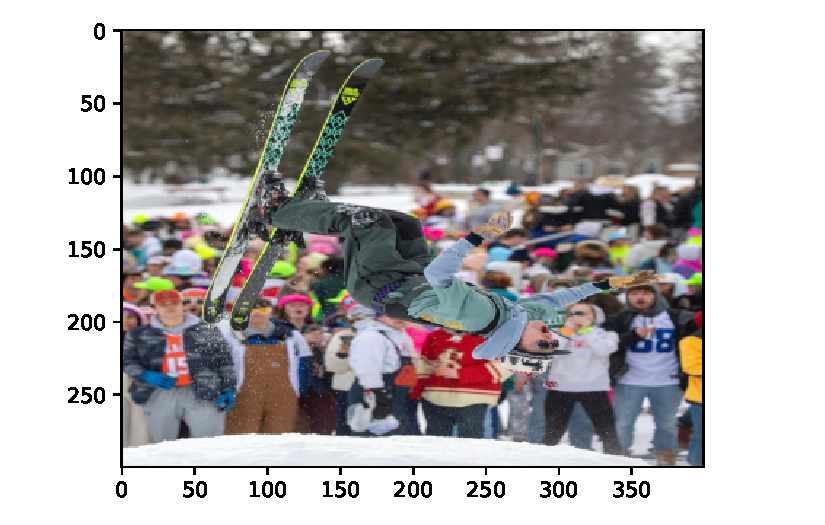
\includegraphics{results_files/figure-pdf/unnamed-chunk-34-10.pdf}

}

\end{figure}

\begin{Shaded}
\begin{Highlighting}[]
\CommentTok{\# hog\_df \textless{}{-} py$hog\_df}


\CommentTok{\# ggplot(hog\_df \%\textgreater{}\% filter(mag \textgreater{}= 0.4), }
\CommentTok{\#        aes(x = radian)) +}
\CommentTok{\#   geom\_histogram(\#binwidth = 5\#, boundary = 0, closed = "right") +}
\CommentTok{\#   )+}
\CommentTok{\#   \#scale\_x\_continuous(limits = c(0, 360), breaks = seq(0, 360, by = 45)) +}
\CommentTok{\#   \#coord\_polar(start = 0, direction = 1, ) +}
\CommentTok{\#   coord\_radial(start = 0, end = pi, expand = F, clip = "on") +}
\CommentTok{\#   scale\_x\_continuous(}
\CommentTok{\#     breaks = c(0, pi/4, pi/2, 3*pi/4), }
\CommentTok{\#     labels = c("0", "π/4", "π/2", "3π/4")}
\CommentTok{\#   ) +}
\CommentTok{\#   theme(plot.title = element\_text(hjust = 0.5)) +}
\CommentTok{\#   labs(title = "Polar Histogram of Theta",}
\CommentTok{\#        x = "Theta (Degrees)",}
\CommentTok{\#        y = "Frequency") \#+ theme\_minimal()}
\end{Highlighting}
\end{Shaded}

\bookmarksetup{startatroot}

\hypertarget{conclusion}{%
\chapter{Conclusion}\label{conclusion}}



\end{document}
